% Options for packages loaded elsewhere
\PassOptionsToPackage{unicode}{hyperref}
\PassOptionsToPackage{hyphens}{url}
\PassOptionsToPackage{dvipsnames,svgnames,x11names}{xcolor}
%
\documentclass[
  letterpaper,
  DIV=11,
  numbers=noendperiod]{scrreprt}

\usepackage{amsmath,amssymb}
\usepackage{iftex}
\ifPDFTeX
  \usepackage[T1]{fontenc}
  \usepackage[utf8]{inputenc}
  \usepackage{textcomp} % provide euro and other symbols
\else % if luatex or xetex
  \usepackage{unicode-math}
  \defaultfontfeatures{Scale=MatchLowercase}
  \defaultfontfeatures[\rmfamily]{Ligatures=TeX,Scale=1}
\fi
\usepackage{lmodern}
\ifPDFTeX\else  
    % xetex/luatex font selection
\fi
% Use upquote if available, for straight quotes in verbatim environments
\IfFileExists{upquote.sty}{\usepackage{upquote}}{}
\IfFileExists{microtype.sty}{% use microtype if available
  \usepackage[]{microtype}
  \UseMicrotypeSet[protrusion]{basicmath} % disable protrusion for tt fonts
}{}
\makeatletter
\@ifundefined{KOMAClassName}{% if non-KOMA class
  \IfFileExists{parskip.sty}{%
    \usepackage{parskip}
  }{% else
    \setlength{\parindent}{0pt}
    \setlength{\parskip}{6pt plus 2pt minus 1pt}}
}{% if KOMA class
  \KOMAoptions{parskip=half}}
\makeatother
\usepackage{xcolor}
\setlength{\emergencystretch}{3em} % prevent overfull lines
\setcounter{secnumdepth}{5}
% Make \paragraph and \subparagraph free-standing
\makeatletter
\ifx\paragraph\undefined\else
  \let\oldparagraph\paragraph
  \renewcommand{\paragraph}{
    \@ifstar
      \xxxParagraphStar
      \xxxParagraphNoStar
  }
  \newcommand{\xxxParagraphStar}[1]{\oldparagraph*{#1}\mbox{}}
  \newcommand{\xxxParagraphNoStar}[1]{\oldparagraph{#1}\mbox{}}
\fi
\ifx\subparagraph\undefined\else
  \let\oldsubparagraph\subparagraph
  \renewcommand{\subparagraph}{
    \@ifstar
      \xxxSubParagraphStar
      \xxxSubParagraphNoStar
  }
  \newcommand{\xxxSubParagraphStar}[1]{\oldsubparagraph*{#1}\mbox{}}
  \newcommand{\xxxSubParagraphNoStar}[1]{\oldsubparagraph{#1}\mbox{}}
\fi
\makeatother

\usepackage{color}
\usepackage{fancyvrb}
\newcommand{\VerbBar}{|}
\newcommand{\VERB}{\Verb[commandchars=\\\{\}]}
\DefineVerbatimEnvironment{Highlighting}{Verbatim}{commandchars=\\\{\}}
% Add ',fontsize=\small' for more characters per line
\usepackage{framed}
\definecolor{shadecolor}{RGB}{241,243,245}
\newenvironment{Shaded}{\begin{snugshade}}{\end{snugshade}}
\newcommand{\AlertTok}[1]{\textcolor[rgb]{0.68,0.00,0.00}{#1}}
\newcommand{\AnnotationTok}[1]{\textcolor[rgb]{0.37,0.37,0.37}{#1}}
\newcommand{\AttributeTok}[1]{\textcolor[rgb]{0.40,0.45,0.13}{#1}}
\newcommand{\BaseNTok}[1]{\textcolor[rgb]{0.68,0.00,0.00}{#1}}
\newcommand{\BuiltInTok}[1]{\textcolor[rgb]{0.00,0.23,0.31}{#1}}
\newcommand{\CharTok}[1]{\textcolor[rgb]{0.13,0.47,0.30}{#1}}
\newcommand{\CommentTok}[1]{\textcolor[rgb]{0.37,0.37,0.37}{#1}}
\newcommand{\CommentVarTok}[1]{\textcolor[rgb]{0.37,0.37,0.37}{\textit{#1}}}
\newcommand{\ConstantTok}[1]{\textcolor[rgb]{0.56,0.35,0.01}{#1}}
\newcommand{\ControlFlowTok}[1]{\textcolor[rgb]{0.00,0.23,0.31}{\textbf{#1}}}
\newcommand{\DataTypeTok}[1]{\textcolor[rgb]{0.68,0.00,0.00}{#1}}
\newcommand{\DecValTok}[1]{\textcolor[rgb]{0.68,0.00,0.00}{#1}}
\newcommand{\DocumentationTok}[1]{\textcolor[rgb]{0.37,0.37,0.37}{\textit{#1}}}
\newcommand{\ErrorTok}[1]{\textcolor[rgb]{0.68,0.00,0.00}{#1}}
\newcommand{\ExtensionTok}[1]{\textcolor[rgb]{0.00,0.23,0.31}{#1}}
\newcommand{\FloatTok}[1]{\textcolor[rgb]{0.68,0.00,0.00}{#1}}
\newcommand{\FunctionTok}[1]{\textcolor[rgb]{0.28,0.35,0.67}{#1}}
\newcommand{\ImportTok}[1]{\textcolor[rgb]{0.00,0.46,0.62}{#1}}
\newcommand{\InformationTok}[1]{\textcolor[rgb]{0.37,0.37,0.37}{#1}}
\newcommand{\KeywordTok}[1]{\textcolor[rgb]{0.00,0.23,0.31}{\textbf{#1}}}
\newcommand{\NormalTok}[1]{\textcolor[rgb]{0.00,0.23,0.31}{#1}}
\newcommand{\OperatorTok}[1]{\textcolor[rgb]{0.37,0.37,0.37}{#1}}
\newcommand{\OtherTok}[1]{\textcolor[rgb]{0.00,0.23,0.31}{#1}}
\newcommand{\PreprocessorTok}[1]{\textcolor[rgb]{0.68,0.00,0.00}{#1}}
\newcommand{\RegionMarkerTok}[1]{\textcolor[rgb]{0.00,0.23,0.31}{#1}}
\newcommand{\SpecialCharTok}[1]{\textcolor[rgb]{0.37,0.37,0.37}{#1}}
\newcommand{\SpecialStringTok}[1]{\textcolor[rgb]{0.13,0.47,0.30}{#1}}
\newcommand{\StringTok}[1]{\textcolor[rgb]{0.13,0.47,0.30}{#1}}
\newcommand{\VariableTok}[1]{\textcolor[rgb]{0.07,0.07,0.07}{#1}}
\newcommand{\VerbatimStringTok}[1]{\textcolor[rgb]{0.13,0.47,0.30}{#1}}
\newcommand{\WarningTok}[1]{\textcolor[rgb]{0.37,0.37,0.37}{\textit{#1}}}

\providecommand{\tightlist}{%
  \setlength{\itemsep}{0pt}\setlength{\parskip}{0pt}}\usepackage{longtable,booktabs,array}
\usepackage{calc} % for calculating minipage widths
% Correct order of tables after \paragraph or \subparagraph
\usepackage{etoolbox}
\makeatletter
\patchcmd\longtable{\par}{\if@noskipsec\mbox{}\fi\par}{}{}
\makeatother
% Allow footnotes in longtable head/foot
\IfFileExists{footnotehyper.sty}{\usepackage{footnotehyper}}{\usepackage{footnote}}
\makesavenoteenv{longtable}
\usepackage{graphicx}
\makeatletter
\def\maxwidth{\ifdim\Gin@nat@width>\linewidth\linewidth\else\Gin@nat@width\fi}
\def\maxheight{\ifdim\Gin@nat@height>\textheight\textheight\else\Gin@nat@height\fi}
\makeatother
% Scale images if necessary, so that they will not overflow the page
% margins by default, and it is still possible to overwrite the defaults
% using explicit options in \includegraphics[width, height, ...]{}
\setkeys{Gin}{width=\maxwidth,height=\maxheight,keepaspectratio}
% Set default figure placement to htbp
\makeatletter
\def\fps@figure{htbp}
\makeatother

\KOMAoption{captions}{tableheading}
\makeatletter
\@ifpackageloaded{tcolorbox}{}{\usepackage[skins,breakable]{tcolorbox}}
\@ifpackageloaded{fontawesome5}{}{\usepackage{fontawesome5}}
\definecolor{quarto-callout-color}{HTML}{909090}
\definecolor{quarto-callout-note-color}{HTML}{0758E5}
\definecolor{quarto-callout-important-color}{HTML}{CC1914}
\definecolor{quarto-callout-warning-color}{HTML}{EB9113}
\definecolor{quarto-callout-tip-color}{HTML}{00A047}
\definecolor{quarto-callout-caution-color}{HTML}{FC5300}
\definecolor{quarto-callout-color-frame}{HTML}{acacac}
\definecolor{quarto-callout-note-color-frame}{HTML}{4582ec}
\definecolor{quarto-callout-important-color-frame}{HTML}{d9534f}
\definecolor{quarto-callout-warning-color-frame}{HTML}{f0ad4e}
\definecolor{quarto-callout-tip-color-frame}{HTML}{02b875}
\definecolor{quarto-callout-caution-color-frame}{HTML}{fd7e14}
\makeatother
\makeatletter
\@ifpackageloaded{bookmark}{}{\usepackage{bookmark}}
\makeatother
\makeatletter
\@ifpackageloaded{caption}{}{\usepackage{caption}}
\AtBeginDocument{%
\ifdefined\contentsname
  \renewcommand*\contentsname{Table of contents}
\else
  \newcommand\contentsname{Table of contents}
\fi
\ifdefined\listfigurename
  \renewcommand*\listfigurename{List of Figures}
\else
  \newcommand\listfigurename{List of Figures}
\fi
\ifdefined\listtablename
  \renewcommand*\listtablename{List of Tables}
\else
  \newcommand\listtablename{List of Tables}
\fi
\ifdefined\figurename
  \renewcommand*\figurename{Figure}
\else
  \newcommand\figurename{Figure}
\fi
\ifdefined\tablename
  \renewcommand*\tablename{Table}
\else
  \newcommand\tablename{Table}
\fi
}
\@ifpackageloaded{float}{}{\usepackage{float}}
\floatstyle{ruled}
\@ifundefined{c@chapter}{\newfloat{codelisting}{h}{lop}}{\newfloat{codelisting}{h}{lop}[chapter]}
\floatname{codelisting}{Listing}
\newcommand*\listoflistings{\listof{codelisting}{List of Listings}}
\makeatother
\makeatletter
\makeatother
\makeatletter
\@ifpackageloaded{caption}{}{\usepackage{caption}}
\@ifpackageloaded{subcaption}{}{\usepackage{subcaption}}
\makeatother

\ifLuaTeX
  \usepackage{selnolig}  % disable illegal ligatures
\fi
\usepackage{bookmark}

\IfFileExists{xurl.sty}{\usepackage{xurl}}{} % add URL line breaks if available
\urlstyle{same} % disable monospaced font for URLs
\hypersetup{
  pdftitle={Vorlesung Ingenieurinformatik},
  pdfauthor={Lukas Arnold; Simone Arnold; Florian Bagemihl; Matthias Baitsch; Marc Fehr; Maik Poetzsch; Sebastian Seipel},
  colorlinks=true,
  linkcolor={blue},
  filecolor={Maroon},
  citecolor={Blue},
  urlcolor={Blue},
  pdfcreator={LaTeX via pandoc}}


\title{Vorlesung Ingenieurinformatik}
\author{Lukas Arnold \and Simone Arnold \and Florian
Bagemihl \and Matthias Baitsch \and Marc Fehr \and Maik
Poetzsch \and Sebastian Seipel}
\date{2025-04-21}

\begin{document}
\maketitle

\renewcommand*\contentsname{Table of contents}
{
\hypersetup{linkcolor=}
\setcounter{tocdepth}{2}
\tableofcontents
}

\bookmarksetup{startatroot}

\chapter*{Preface}\label{preface}
\addcontentsline{toc}{chapter}{Preface}

\markboth{Preface}{Preface}

This is a Quarto book.

To learn more about Quarto books visit
\url{https://quarto.org/docs/books}.

\part{w-python}

\chapter*{Werkzeugbaustein Python}\label{werkzeugbaustein-python}
\addcontentsline{toc}{chapter}{Werkzeugbaustein Python}

\markboth{Werkzeugbaustein Python}{Werkzeugbaustein Python}

\phantomsection\label{Lizenz}
\begin{figure}

\begin{minipage}{0.20\linewidth}

\includegraphics{index_files/mediabag/books/w-python/skript/00-bilder/CC-BY.pdf}\end{minipage}%
%
\begin{minipage}{0.80\linewidth}
Bausteine Computergestützter Datenanalyse von Lukas Arnold, Simone
Arnold, Florian Bagemihl, Matthias Baitsch, Marc Fehr, Maik Poetzsch und
Sebastian Seipel. Werkzeugbaustein Python von Maik Poetzsch ist
lizensiert unter
\href{https://creativecommons.org/licenses/by/4.0/deed.de}{CC BY 4.0}.
Das Werk ist abrufbar auf
\href{https://github.com/bausteine-der-datenanalyse/w-python}{GitHub}.
Ausgenommen von der Lizenz sind alle Logos Dritter und anders
gekennzeichneten Inhalte. 2025\end{minipage}%

\end{figure}%

Zitiervorschlag

Arnold, Lukas, Simone Arnold, Matthias Baitsch, Marc Fehr, Maik
Poetzsch, und Sebastian Seipel. 2025. „Bausteine Computergestützter
Datenanalyse. Werkzeugbaustein Python``.
\url{https://github.com/bausteine-der-datenanalyse/w-python}.

BibTeX-Vorlage

\begin{verbatim}
@misc{BCD-w-python-2025,
 title={Bausteine Computergestützter Datenanalyse. Werkzeugbaustein Python},
 author={Arnold, Lukas and Arnold, Simone and Baitsch, Matthias and Fehr, Marc and Poetzsch, Maik and Seipel, Sebastian},
 year={2025},
 url={https://github.com/bausteine-der-datenanalyse/w-python}} 
\end{verbatim}

\section*{Voraussetzungen}\label{voraussetzungen}
\addcontentsline{toc}{section}{Voraussetzungen}

\markright{Voraussetzungen}

Keine Voraussetzungen

\section*{Lernziele}\label{lernziele}
\addcontentsline{toc}{section}{Lernziele}

\markright{Lernziele}

In diesem Bausteine werden die Grundzüge der Programmierung mit Python
vermittelt. In diesem Baustein lernen Sie \ldots{}

\begin{itemize}
\item
  Grundlagen des Programmierens
\item
  Ausgaben in Python, Grundlegende Datentypen, FLusskontrolle
\item
  die Dokumentation zu lesen und zu verwenden
\item
  Module und Pakete laden
\end{itemize}

\chapter{Einleitung: Datenanalyse mit
Python}\label{einleitung-datenanalyse-mit-python}

\begin{figure}[H]

{\centering 
\includegraphics{books/w-python/skript/00-bilder/python-logo-and-wordmark-cc0-tm.png}

}

\caption{Logo der Programmiersprache Python}

\end{figure}%

Python Logo von Python Software Foundation steht unter der
\href{https://www.gnu.org/licenses/gpl-3.0.html}{GPLv3}. Die
Wort-Bild-Marke ist markenrechtlich geschützt:
\url{https://www.python.org/psf/trademarks/}. Das Werk ist abrufbar auf
\href{https://de.m.wikipedia.org/wiki/Datei:Python_logo_and_wordmark.svg}{wikimedia}.
2008

\chapter{Willkommen bei Python!}\label{willkommen-bei-python}

Python ist eine moderne Programmiersprache, die sich besonders gut für
Einsteigerinnen und Einsteiger eignet. Sie ist leicht verständlich und
wird in vielen Bereichen eingesetzt -- von der Datenanalyse bis hin zur
Webentwicklung.

\begin{quote}
In diesem Kurs lernen Sie Python Schritt für Schritt anhand praktischer
Beispiele.
\end{quote}

\begin{center}\rule{0.5\linewidth}{0.5pt}\end{center}

\section{Lernziele dieses Kapitels}\label{lernziele-dieses-kapitels}

Am Ende dieses Kapitels können Sie: - einfache Python-Programme
schreiben, - Text auf dem Bildschirm ausgeben, - erste Variablen
definieren und verwenden.

\begin{center}\rule{0.5\linewidth}{0.5pt}\end{center}

\section{Ihr erstes Programm}\label{ihr-erstes-programm}

Die ersten Schritte in einer neuen Programmiersprache sind immer die
gleichen. WIr lassen uns die Worte `Hello World' ausgeben. Dazu nutzen
wir den print-Befehl \texttt{print(...)}:

\begin{Shaded}
\begin{Highlighting}[]
\BuiltInTok{print}\NormalTok{(}\StringTok{"Hallo Welt!"}\NormalTok{)}
\end{Highlighting}
\end{Shaded}

\begin{verbatim}
Hallo Welt!
\end{verbatim}

\textbf{Was passiert hier?} - \texttt{print(...)} ist eine sogenannte
\textbf{Funktion}, die etwas auf dem Bildschirm ausgibt. - Der Text
\texttt{"Hello\ World!"} wird angezeigt. - Texte (auch „Strings``
genannt) stehen immer in Anführungszeichen.

\section{Variablen -- Namen für
Werte}\label{variablen-namen-fuxfcr-werte}

Variablen sind wie beschriftete Schubladen: Sie speichern Informationen
unter einem Namen.

\begin{Shaded}
\begin{Highlighting}[]
\NormalTok{name }\OperatorTok{=} \StringTok{"Frau Müller"}
\NormalTok{alter }\OperatorTok{=} \DecValTok{32}
\end{Highlighting}
\end{Shaded}

Sie können diese Variablen verwenden, um dynamische Ausgaben zu
erzeugen:

\begin{Shaded}
\begin{Highlighting}[]
\BuiltInTok{print}\NormalTok{(name }\OperatorTok{+} \StringTok{" ist "} \OperatorTok{+} \BuiltInTok{str}\NormalTok{(alter) }\OperatorTok{+} \StringTok{" Jahre alt."}\NormalTok{)}
\end{Highlighting}
\end{Shaded}

\begin{verbatim}
Frau Müller ist 32 Jahre alt.
\end{verbatim}

Zu beachten ist hier, dass sie versuchen sowohl eine Zahl, als auch Text
auszugeben. Daher müssen wir mit der Funktion `str()' die Zahl in Text
umwandeln.

\begin{tcolorbox}[enhanced jigsaw, breakable, opacityback=0, left=2mm, coltitle=black, leftrule=.75mm, colframe=quarto-callout-tip-color-frame, opacitybacktitle=0.6, toprule=.15mm, bottomtitle=1mm, titlerule=0mm, toptitle=1mm, title=\textcolor{quarto-callout-tip-color}{\faLightbulb}\hspace{0.5em}{✏️ Aufgabe: Begrüßung mit Alter}, colbacktitle=quarto-callout-tip-color!10!white, arc=.35mm, bottomrule=.15mm, rightrule=.15mm, colback=white]

Schreiben Sie ein Programm, das Sie mit Ihrem Namen begrüßt:

\begin{verbatim}
Hallo Frau Müller!
\end{verbatim}

Tipp: In Python können Sie Texte mit \texttt{+} zusammenfügen. Denken
Sie daran, dass Strings in Anführungszeichen stehen müssen.

\begin{tcolorbox}[enhanced jigsaw, breakable, opacityback=0, left=2mm, coltitle=black, leftrule=.75mm, colframe=quarto-callout-caution-color-frame, opacitybacktitle=0.6, toprule=.15mm, bottomtitle=1mm, titlerule=0mm, toptitle=1mm, title={Lösung}, colbacktitle=quarto-callout-caution-color!10!white, arc=.35mm, bottomrule=.15mm, rightrule=.15mm, colback=white]

\begin{Shaded}
\begin{Highlighting}[]
\NormalTok{mein\_name }\OperatorTok{=} \StringTok{"Ihr Name hier"}
\BuiltInTok{print}\NormalTok{(}\StringTok{"Hallo "} \OperatorTok{+}\NormalTok{ mein\_name }\OperatorTok{+} \StringTok{"!"}\NormalTok{)}
\end{Highlighting}
\end{Shaded}

\begin{verbatim}
Hallo Ihr Name hier!
\end{verbatim}

\end{tcolorbox}

Erweitern Sie Ihr Programm so, dass es eine Begrüßung inklusive Alter
ausgibt:

\begin{verbatim}
Hallo Frau Müller!
Sie sind 32 Jahre alt.
\end{verbatim}

Tipp: Verwenden Sie \texttt{print(...)} mehrmals oder fügen Sie Texte
zusammen.

\begin{tcolorbox}[enhanced jigsaw, breakable, opacityback=0, left=2mm, coltitle=black, leftrule=.75mm, colframe=quarto-callout-caution-color-frame, opacitybacktitle=0.6, toprule=.15mm, bottomtitle=1mm, titlerule=0mm, toptitle=1mm, title={Lösung}, colbacktitle=quarto-callout-caution-color!10!white, arc=.35mm, bottomrule=.15mm, rightrule=.15mm, colback=white]

\begin{Shaded}
\begin{Highlighting}[]
\NormalTok{name }\OperatorTok{=} \StringTok{"Frau Müller"}
\NormalTok{alter }\OperatorTok{=} \DecValTok{32}

\BuiltInTok{print}\NormalTok{(}\StringTok{"Hallo "} \OperatorTok{+}\NormalTok{ name }\OperatorTok{+} \StringTok{"!"}\NormalTok{)}
\BuiltInTok{print}\NormalTok{(}\StringTok{"Sie sind "} \OperatorTok{+} \BuiltInTok{str}\NormalTok{(alter) }\OperatorTok{+} \StringTok{" Jahre alt."}\NormalTok{)}
\end{Highlighting}
\end{Shaded}

\begin{verbatim}
Hallo Frau Müller!
Sie sind 32 Jahre alt.
\end{verbatim}

\end{tcolorbox}

\end{tcolorbox}

\chapter{Einführung: Datentypen
verstehen}\label{einfuxfchrung-datentypen-verstehen}

\section{Lernziele dieses Kapitels}\label{lernziele-dieses-kapitels-1}

Am Ende dieses Kapitels können Sie: - die wichtigsten Datentypen
unterscheiden, - mit Zahlen und Texten rechnen bzw. arbeiten, - einfache
Berechnungen und Ausgaben erstellen.

\section{Einleitung}\label{einleitung}

In Python gibt es verschiedene \textbf{Datentypen}. Diese beschreiben,
\textbf{welche Art von Daten} Sie in Variablen speichern. Das ist
wichtig, weil viele Operationen -- wie zum Beispiel \texttt{+} -- je
nach Datentyp etwas anderes bedeuten:

\begin{itemize}
\tightlist
\item
  \texttt{+} bei Zahlen bedeutet \textbf{Addition},
\item
  \texttt{+} bei Text bedeutet \textbf{Zusammenfügen} (Konkatenation).
\end{itemize}

Bevor wir also mit komplexeren Programmen arbeiten, sollten wir
verstehen, welche Datentypen es gibt und wie man mit ihnen umgeht.

\section{Die wichtigsten Datentypen}\label{die-wichtigsten-datentypen}

Hier sind die grundlegenden Datentypen in Python:

\begin{longtable}[]{@{}lll@{}}
\toprule\noalign{}
Typ & Beispiel & Bedeutung \\
\midrule\noalign{}
\endhead
\bottomrule\noalign{}
\endlastfoot
\texttt{int} & \texttt{10} & Ganze Zahl \\
\texttt{float} & \texttt{3.14} & Kommazahl \\
\texttt{str} & \texttt{"Hallo"} & Text (String) \\
\texttt{bool} & \texttt{True}, \texttt{False} & Wahrheitswert
(Ja/Nein) \\
\end{longtable}

Sie können den Typ einer Variable mit der Funktion \texttt{type(...)}
herausfinden:

\begin{Shaded}
\begin{Highlighting}[]
\NormalTok{wert }\OperatorTok{=} \DecValTok{42}
\BuiltInTok{print}\NormalTok{(}\BuiltInTok{type}\NormalTok{(wert))  }\CommentTok{\# Ausgabe: \textless{}class \textquotesingle{}int\textquotesingle{}\textgreater{}}
\end{Highlighting}
\end{Shaded}

\begin{verbatim}
<class 'int'>
\end{verbatim}

\begin{center}\rule{0.5\linewidth}{0.5pt}\end{center}

\section{\texorpdfstring{🔍 Unterschiede zwischen \texttt{int} und
\texttt{float}}{🔍 Unterschiede zwischen int und float}}\label{unterschiede-zwischen-int-und-float}

In Python unterscheidet man zwischen \textbf{ganzen Zahlen}
(\texttt{int}) und \textbf{Kommazahlen} (\texttt{float}):

\begin{itemize}
\tightlist
\item
  \texttt{int} steht für „integer`` -- also ganze Zahlen wie \texttt{1},
  \texttt{0}, \texttt{-10}
\item
  \texttt{float} steht für „floating point number`` -- also Zahlen mit
  Dezimalstellen wie \texttt{3.14}, \texttt{0.5}, \texttt{-2.0}
\end{itemize}

\begin{Shaded}
\begin{Highlighting}[]
\NormalTok{a }\OperatorTok{=} \DecValTok{10}       \CommentTok{\# int}
\NormalTok{b }\OperatorTok{=} \FloatTok{2.5}      \CommentTok{\# float}

\BuiltInTok{print}\NormalTok{(}\StringTok{"a:"}\NormalTok{, a, }\StringTok{"| Typ:"}\NormalTok{, }\BuiltInTok{type}\NormalTok{(a))}
\BuiltInTok{print}\NormalTok{(}\StringTok{"b:"}\NormalTok{, b, }\StringTok{"| Typ:"}\NormalTok{, }\BuiltInTok{type}\NormalTok{(b))}
\end{Highlighting}
\end{Shaded}

\begin{verbatim}
a: 10 | Typ: <class 'int'>
b: 2.5 | Typ: <class 'float'>
\end{verbatim}

💡 Die Unterscheidung ist wichtig: Manche Rechenoperationen verhalten
sich je nach Datentyp leicht unterschiedlich.

\section{\texorpdfstring{🔍 Was sind Booleans
(\texttt{bool})?}{🔍 Was sind Booleans (bool)?}}\label{was-sind-booleans-bool}

Ein \textbf{Boolean} ist ein Wahrheitswert: Er kann nur zwei Zustände
annehmen:

\begin{itemize}
\tightlist
\item
  \texttt{True} (wahr)
\item
  \texttt{False} (falsch)
\end{itemize}

Solche Werte begegnen uns zum Beispiel bei Fragen wie:

\begin{itemize}
\tightlist
\item
  Ist die Temperatur über 30\,°C?
\item
  Hat die Datei einen bestimmten Namen?
\item
  Ist die Liste leer?
\end{itemize}

\begin{Shaded}
\begin{Highlighting}[]
\NormalTok{ist\_sonnig }\OperatorTok{=} \VariableTok{True}
\NormalTok{hat\_regenschirm }\OperatorTok{=} \VariableTok{False}

\BuiltInTok{print}\NormalTok{(}\StringTok{"Sonnig:"}\NormalTok{, ist\_sonnig)}
\BuiltInTok{print}\NormalTok{(}\StringTok{"Regenschirm dabei?"}\NormalTok{, hat\_regenschirm)}
\BuiltInTok{print}\NormalTok{(}\StringTok{"Typ von \textquotesingle{}ist\_sonnig\textquotesingle{}:"}\NormalTok{, }\BuiltInTok{type}\NormalTok{(ist\_sonnig))}
\end{Highlighting}
\end{Shaded}

\begin{verbatim}
Sonnig: True
Regenschirm dabei? False
Typ von 'ist_sonnig': <class 'bool'>
\end{verbatim}

Booleans werden besonders in \textbf{Bedingungen} und
\textbf{Vergleichen} verwendet, was Sie in Kapitel 4 genauer
kennenlernen.

\begin{center}\rule{0.5\linewidth}{0.5pt}\end{center}

\section{Rechnen mit Zahlen}\label{rechnen-mit-zahlen}

Python kann wie ein Taschenrechner verwendet werden:

\begin{longtable}[]{@{}cc@{}}
\toprule\noalign{}
Operator & Beschreibung \\
\midrule\noalign{}
\endhead
\bottomrule\noalign{}
\endlastfoot
\texttt{+}, \texttt{-} & Addition / Subtraktion \\
\texttt{*}, \texttt{/} & Multiplikation / Division \\
\texttt{//}, \texttt{\%} & Ganzzahlige Division / Rest \\
\texttt{**} & Potenzieren \\
\end{longtable}

\begin{Shaded}
\begin{Highlighting}[]
\NormalTok{a }\OperatorTok{=} \DecValTok{10}
\NormalTok{b }\OperatorTok{=} \DecValTok{3}

\BuiltInTok{print}\NormalTok{(}\StringTok{"Addition:"}\NormalTok{, a }\OperatorTok{+}\NormalTok{ b)}
\BuiltInTok{print}\NormalTok{(}\StringTok{"Subtraktion:"}\NormalTok{, a }\OperatorTok{{-}}\NormalTok{ b)}
\BuiltInTok{print}\NormalTok{(}\StringTok{"Multiplikation:"}\NormalTok{, a }\OperatorTok{*}\NormalTok{ b)}
\BuiltInTok{print}\NormalTok{(}\StringTok{"Potenzieren"}\NormalTok{, a}\OperatorTok{**}\NormalTok{b)}
\BuiltInTok{print}\NormalTok{(}\StringTok{"Division:"}\NormalTok{, a }\OperatorTok{/}\NormalTok{ b)}
\BuiltInTok{print}\NormalTok{(}\StringTok{"Ganzzahlige Division:"}\NormalTok{, a }\OperatorTok{//}\NormalTok{ b)}
\BuiltInTok{print}\NormalTok{(}\StringTok{"Division mit Rest:"}\NormalTok{, a }\OperatorTok{\%}\NormalTok{ b)}
\end{Highlighting}
\end{Shaded}

\begin{verbatim}
Addition: 13
Subtraktion: 7
Multiplikation: 30
Potenzieren 1000
Division: 3.3333333333333335
Ganzzahlige Division: 3
Division mit Rest: 1
\end{verbatim}

💡 \texttt{//} bedeutet: Ganzzahldivision, das Ergebnis wird abgerundet.
Alternativ gibt es auch \texttt{\%}. Hier wird eine Ganzzahldivision
durchgeführt und der Rest ausgegeben.

\begin{center}\rule{0.5\linewidth}{0.5pt}\end{center}

\section{Arbeiten mit Text}\label{arbeiten-mit-text}

Texte (Strings) können miteinander kombiniert werden:

\begin{Shaded}
\begin{Highlighting}[]
\NormalTok{vorname }\OperatorTok{=} \StringTok{"Anna"}
\NormalTok{nachname }\OperatorTok{=} \StringTok{"Beispiel"}
\BuiltInTok{print}\NormalTok{(}\StringTok{"Willkommen, "} \OperatorTok{+}\NormalTok{ vorname }\OperatorTok{+} \StringTok{" "} \OperatorTok{+}\NormalTok{ nachname }\OperatorTok{+} \StringTok{"!"}\NormalTok{)}
\end{Highlighting}
\end{Shaded}

\begin{verbatim}
Willkommen, Anna Beispiel!
\end{verbatim}

Wenn Sie Text und Zahlen kombinieren wollen, müssen Sie die Zahl in
einen String umwandeln:

\begin{Shaded}
\begin{Highlighting}[]
\NormalTok{punkte }\OperatorTok{=} \DecValTok{95}
\BuiltInTok{print}\NormalTok{(}\StringTok{"Sie haben "} \OperatorTok{+} \BuiltInTok{str}\NormalTok{(punkte) }\OperatorTok{+} \StringTok{" Punkte erreicht."}\NormalTok{)}
\end{Highlighting}
\end{Shaded}

\begin{verbatim}
Sie haben 95 Punkte erreicht.
\end{verbatim}

\section{🔁 Umwandlung von Datentypen
(Typecasting)}\label{umwandlung-von-datentypen-typecasting}

Manchmal müssen Sie einen Wert von einem Datentyp in einen anderen
umwandeln -- z.\,B. eine Zahl in einen Text (String), damit sie
ausgegeben werden kann.

Das nennt man \textbf{Typecasting}. Hier sind die wichtigsten Funktionen
dafür:

\begin{longtable}[]{@{}lll@{}}
\toprule\noalign{}
Funktion & Beschreibung & Beispiel \\
\midrule\noalign{}
\endhead
\bottomrule\noalign{}
\endlastfoot
\texttt{str(...)} & Zahl → Text & \texttt{str(42)} → \texttt{"42"} \\
\texttt{int(...)} & Text/Zahl → ganze Zahl & \texttt{int("10")} →
\texttt{10} \\
\texttt{float(...)} & Text/Zahl → Kommazahl & \texttt{float("3.14")} →
\texttt{3.14} \\
\end{longtable}

\begin{Shaded}
\begin{Highlighting}[]
\CommentTok{\# Beispiel: Zahl als Text anzeigen}
\NormalTok{punkte }\OperatorTok{=} \DecValTok{100}
\BuiltInTok{print}\NormalTok{(}\StringTok{"Sie haben "} \OperatorTok{+} \BuiltInTok{str}\NormalTok{(punkte) }\OperatorTok{+} \StringTok{" Punkte."}\NormalTok{)}

\CommentTok{\# Beispiel: String in Zahl umwandeln und berechnen}
\NormalTok{eingabe }\OperatorTok{=} \StringTok{"3.5"}
\NormalTok{wert }\OperatorTok{=} \BuiltInTok{float}\NormalTok{(eingabe) }\OperatorTok{*} \DecValTok{2}
\BuiltInTok{print}\NormalTok{(}\StringTok{"Doppelt so viel:"}\NormalTok{, wert)}
\end{Highlighting}
\end{Shaded}

\begin{verbatim}
Sie haben 100 Punkte.
Doppelt so viel: 7.0
\end{verbatim}

💡 Achten Sie beim Umwandeln darauf, dass der Inhalt auch wirklich passt
-- \texttt{int("abc")} führt zu einem Fehler.

\begin{tcolorbox}[enhanced jigsaw, breakable, opacityback=0, left=2mm, coltitle=black, leftrule=.75mm, colframe=quarto-callout-tip-color-frame, opacitybacktitle=0.6, toprule=.15mm, bottomtitle=1mm, titlerule=0mm, toptitle=1mm, title=\textcolor{quarto-callout-tip-color}{\faLightbulb}\hspace{0.5em}{✏️ Aufgabe: Alter in Tagen}, colbacktitle=quarto-callout-tip-color!10!white, arc=.35mm, bottomrule=.15mm, rightrule=.15mm, colback=white]

Berechnen Sie, wie alt eine Person in Tagen ist.

\begin{Shaded}
\begin{Highlighting}[]
\NormalTok{alter\_jahre }\OperatorTok{=} \DecValTok{32}
\NormalTok{tage }\OperatorTok{=}\NormalTok{ alter\_jahre }\OperatorTok{*} \DecValTok{365}
\BuiltInTok{print}\NormalTok{(}\StringTok{"Sie sind ungefähr "} \OperatorTok{+} \BuiltInTok{str}\NormalTok{(tage) }\OperatorTok{+} \StringTok{" Tage alt."}\NormalTok{)}
\end{Highlighting}
\end{Shaded}

\begin{verbatim}
Sie sind ungefähr 11680 Tage alt.
\end{verbatim}

Tipp: Denken Sie an die Umwandlung in einen String, wenn Sie die Zahl
ausgeben möchten.

\begin{tcolorbox}[enhanced jigsaw, breakable, opacityback=0, left=2mm, coltitle=black, leftrule=.75mm, colframe=quarto-callout-caution-color-frame, opacitybacktitle=0.6, toprule=.15mm, bottomtitle=1mm, titlerule=0mm, toptitle=1mm, title={Lösung}, colbacktitle=quarto-callout-caution-color!10!white, arc=.35mm, bottomrule=.15mm, rightrule=.15mm, colback=white]

\begin{Shaded}
\begin{Highlighting}[]
\NormalTok{alter }\OperatorTok{=} \DecValTok{32}
\NormalTok{tage }\OperatorTok{=}\NormalTok{ alter }\OperatorTok{*} \DecValTok{365}
\BuiltInTok{print}\NormalTok{(}\StringTok{"Sie sind ungefähr "} \OperatorTok{+} \BuiltInTok{str}\NormalTok{(tage) }\OperatorTok{+} \StringTok{" Tage alt."}\NormalTok{)}
\end{Highlighting}
\end{Shaded}

\begin{verbatim}
Sie sind ungefähr 11680 Tage alt.
\end{verbatim}

\end{tcolorbox}

\end{tcolorbox}

\chapter{Einführung: Entscheidungen und
Wiederholungen}\label{einfuxfchrung-entscheidungen-und-wiederholungen}

Programme müssen oft Entscheidungen treffen -- zum Beispiel abhängig von
einer Benutzereingabe oder einem bestimmten Wert. Ebenso müssen
bestimmte Aktionen mehrfach durchgeführt werden.

Dafür gibt es zwei zentrale Elemente in Python:

\begin{itemize}
\tightlist
\item
  \textbf{Kontrollstrukturen}: \texttt{if}, \texttt{elif}, \texttt{else}
\item
  \textbf{Schleifen}: \texttt{while} und \texttt{for}
\end{itemize}

\begin{center}\rule{0.5\linewidth}{0.5pt}\end{center}

\section{Lernziele dieses Kapitels}\label{lernziele-dieses-kapitels-2}

Am Ende dieses Kapitels können Sie: - Bedingungen formulieren und mit
\texttt{if}, \texttt{elif}, \texttt{else} nutzen, - Vergleichsoperatoren
verwenden (\texttt{==}, \texttt{\textless{}}, \texttt{!=}, \ldots), -
Wiederholungen mit \texttt{while} und \texttt{for} umsetzen.

\begin{center}\rule{0.5\linewidth}{0.5pt}\end{center}

\section{\texorpdfstring{Bedingungen mit \texttt{if}, \texttt{elif},
\texttt{else}}{Bedingungen mit if, elif, else}}\label{bedingungen-mit-if-elif-else}

\begin{Shaded}
\begin{Highlighting}[]
\NormalTok{alter }\OperatorTok{=} \DecValTok{17}

\ControlFlowTok{if}\NormalTok{ alter }\OperatorTok{\textgreater{}=} \DecValTok{18}\NormalTok{:}
    \BuiltInTok{print}\NormalTok{(}\StringTok{"Sie sind volljährig."}\NormalTok{)}
\ControlFlowTok{else}\NormalTok{:}
    \BuiltInTok{print}\NormalTok{(}\StringTok{"Sie sind minderjährig."}\NormalTok{)}
\end{Highlighting}
\end{Shaded}

\begin{verbatim}
Sie sind minderjährig.
\end{verbatim}

Mehrere Fälle unterscheiden:

\begin{Shaded}
\begin{Highlighting}[]
\NormalTok{note }\OperatorTok{=} \FloatTok{2.3}

\ControlFlowTok{if}\NormalTok{ note }\OperatorTok{\textless{}=} \FloatTok{1.5}\NormalTok{:}
    \BuiltInTok{print}\NormalTok{(}\StringTok{"Sehr gut"}\NormalTok{)}
\ControlFlowTok{elif}\NormalTok{ note }\OperatorTok{\textless{}=} \FloatTok{2.5}\NormalTok{:}
    \BuiltInTok{print}\NormalTok{(}\StringTok{"Gut"}\NormalTok{)}
\ControlFlowTok{elif}\NormalTok{ note }\OperatorTok{\textless{}=} \FloatTok{3.5}\NormalTok{:}
    \BuiltInTok{print}\NormalTok{(}\StringTok{"Befriedigend"}\NormalTok{)}
\ControlFlowTok{else}\NormalTok{:}
    \BuiltInTok{print}\NormalTok{(}\StringTok{"Ausreichend oder schlechter"}\NormalTok{)}
\end{Highlighting}
\end{Shaded}

\begin{verbatim}
Gut
\end{verbatim}

\begin{center}\rule{0.5\linewidth}{0.5pt}\end{center}

\section{Vergleichsoperatoren}\label{vergleichsoperatoren}

\begin{longtable}[]{@{}ll@{}}
\toprule\noalign{}
Ausdruck & Bedeutung \\
\midrule\noalign{}
\endhead
\bottomrule\noalign{}
\endlastfoot
\texttt{a\ ==\ b} & gleich \\
\texttt{a\ !=\ b} & ungleich \\
\texttt{a\ \textless{}\ b} & kleiner als \\
\texttt{a\ \textgreater{}\ b} & größer als \\
\texttt{a\ \textless{}=\ b} & kleiner oder gleich \\
\texttt{a\ \textgreater{}=\ b} & größer oder gleich \\
\end{longtable}

\begin{center}\rule{0.5\linewidth}{0.5pt}\end{center}

\section{\texorpdfstring{Wiederholungen mit
\texttt{while}}{Wiederholungen mit while}}\label{wiederholungen-mit-while}

\begin{Shaded}
\begin{Highlighting}[]
\NormalTok{zähler }\OperatorTok{=} \DecValTok{0}

\ControlFlowTok{while}\NormalTok{ zähler }\OperatorTok{\textless{}} \DecValTok{5}\NormalTok{:}
    \BuiltInTok{print}\NormalTok{(}\StringTok{"Zähler ist:"}\NormalTok{, zähler)}
\NormalTok{    zähler }\OperatorTok{+=} \DecValTok{1}
\end{Highlighting}
\end{Shaded}

\begin{verbatim}
Zähler ist: 0
Zähler ist: 1
Zähler ist: 2
Zähler ist: 3
Zähler ist: 4
\end{verbatim}

💡 Achten Sie auf eine Abbruchbedingung -- sonst läuft die Schleife
endlos!

\begin{center}\rule{0.5\linewidth}{0.5pt}\end{center}

\section{\texorpdfstring{Schleifen mit \texttt{for} und
\texttt{range(...)}}{Schleifen mit for und range(...)}}\label{schleifen-mit-for-und-range...}

Wenn Sie eine Schleife \textbf{genau eine bestimmte Anzahl von Malen}
durchlaufen möchten, nutzen Sie \texttt{for} mit \texttt{range(...)}:

\begin{Shaded}
\begin{Highlighting}[]
\ControlFlowTok{for}\NormalTok{ i }\KeywordTok{in} \BuiltInTok{range}\NormalTok{(}\DecValTok{5}\NormalTok{):}
    \BuiltInTok{print}\NormalTok{(}\StringTok{"Durchlauf:"}\NormalTok{, i)}
\end{Highlighting}
\end{Shaded}

\begin{verbatim}
Durchlauf: 0
Durchlauf: 1
Durchlauf: 2
Durchlauf: 3
Durchlauf: 4
\end{verbatim}

Start- und Endwert festlegen:

\begin{Shaded}
\begin{Highlighting}[]
\ControlFlowTok{for}\NormalTok{ i }\KeywordTok{in} \BuiltInTok{range}\NormalTok{(}\DecValTok{1}\NormalTok{, }\DecValTok{6}\NormalTok{):}
    \BuiltInTok{print}\NormalTok{(i)}
\end{Highlighting}
\end{Shaded}

\begin{verbatim}
1
2
3
4
5
\end{verbatim}

\section{\texorpdfstring{Was macht \texttt{range(...)}
genau?}{Was macht range(...) genau?}}\label{was-macht-range...-genau}

Die Funktion \texttt{range(...)} erzeugt eine Abfolge von Zahlen, über
die Sie mit einer \texttt{for}-Schleife iterieren können.

\subsection{🔢 Varianten:}\label{varianten}

\begin{Shaded}
\begin{Highlighting}[]
\BuiltInTok{range}\NormalTok{(}\DecValTok{5}\NormalTok{)}
\end{Highlighting}
\end{Shaded}

➡️ ergibt: \texttt{0,\ 1,\ 2,\ 3,\ 4} (startet bei 0, endet \textbf{vor}
5)

\begin{Shaded}
\begin{Highlighting}[]
\BuiltInTok{range}\NormalTok{(}\DecValTok{2}\NormalTok{, }\DecValTok{6}\NormalTok{)}
\end{Highlighting}
\end{Shaded}

➡️ ergibt: \texttt{2,\ 3,\ 4,\ 5} (startet bei 2, endet \textbf{vor} 6)

\begin{Shaded}
\begin{Highlighting}[]
\BuiltInTok{range}\NormalTok{(}\DecValTok{1}\NormalTok{, }\DecValTok{10}\NormalTok{, }\DecValTok{2}\NormalTok{)}
\end{Highlighting}
\end{Shaded}

➡️ ergibt: \texttt{1,\ 3,\ 5,\ 7,\ 9} (Schrittweite = 2)

💡 \texttt{range(...)} erzeugt keine echte Liste, sondern ein
sogenanntes „range-Objekt``, das wie eine Liste verwendet werden kann.

\begin{tcolorbox}[enhanced jigsaw, breakable, opacityback=0, left=2mm, coltitle=black, leftrule=.75mm, colframe=quarto-callout-tip-color-frame, opacitybacktitle=0.6, toprule=.15mm, bottomtitle=1mm, titlerule=0mm, toptitle=1mm, title=\textcolor{quarto-callout-tip-color}{\faLightbulb}\hspace{0.5em}{✏️ Aufgabe: Zähle von 1 bis 10}, colbacktitle=quarto-callout-tip-color!10!white, arc=.35mm, bottomrule=.15mm, rightrule=.15mm, colback=white]

Nutzen Sie eine \texttt{for}-Schleife, um die Zahlen von 1 bis 10
auszugeben.

\begin{tcolorbox}[enhanced jigsaw, breakable, opacityback=0, left=2mm, coltitle=black, leftrule=.75mm, colframe=quarto-callout-caution-color-frame, opacitybacktitle=0.6, toprule=.15mm, bottomtitle=1mm, titlerule=0mm, toptitle=1mm, title={Lösung}, colbacktitle=quarto-callout-caution-color!10!white, arc=.35mm, bottomrule=.15mm, rightrule=.15mm, colback=white]

\begin{Shaded}
\begin{Highlighting}[]
\ControlFlowTok{for}\NormalTok{ i }\KeywordTok{in} \BuiltInTok{range}\NormalTok{(}\DecValTok{1}\NormalTok{, }\DecValTok{11}\NormalTok{):}
    \BuiltInTok{print}\NormalTok{(i)}
\end{Highlighting}
\end{Shaded}

\begin{verbatim}
1
2
3
4
5
6
7
8
9
10
\end{verbatim}

\end{tcolorbox}

\end{tcolorbox}

\begin{center}\rule{0.5\linewidth}{0.5pt}\end{center}

\begin{tcolorbox}[enhanced jigsaw, breakable, opacityback=0, left=2mm, coltitle=black, leftrule=.75mm, colframe=quarto-callout-tip-color-frame, opacitybacktitle=0.6, toprule=.15mm, bottomtitle=1mm, titlerule=0mm, toptitle=1mm, title=\textcolor{quarto-callout-tip-color}{\faLightbulb}\hspace{0.5em}{✏️ Aufgabe: Gerade Zahlen ausgeben}, colbacktitle=quarto-callout-tip-color!10!white, arc=.35mm, bottomrule=.15mm, rightrule=.15mm, colback=white]

Geben Sie alle geraden Zahlen von 0 bis 20 aus. Tipp: Eine Zahl ist
gerade, wenn \texttt{zahl\ \%\ 2\ ==\ 0}.

\begin{tcolorbox}[enhanced jigsaw, breakable, opacityback=0, left=2mm, coltitle=black, leftrule=.75mm, colframe=quarto-callout-caution-color-frame, opacitybacktitle=0.6, toprule=.15mm, bottomtitle=1mm, titlerule=0mm, toptitle=1mm, title={Lösung}, colbacktitle=quarto-callout-caution-color!10!white, arc=.35mm, bottomrule=.15mm, rightrule=.15mm, colback=white]

\begin{Shaded}
\begin{Highlighting}[]
\ControlFlowTok{for}\NormalTok{ zahl }\KeywordTok{in} \BuiltInTok{range}\NormalTok{(}\DecValTok{0}\NormalTok{, }\DecValTok{21}\NormalTok{):}
    \ControlFlowTok{if}\NormalTok{ zahl }\OperatorTok{\%} \DecValTok{2} \OperatorTok{==} \DecValTok{0}\NormalTok{:}
        \BuiltInTok{print}\NormalTok{(zahl)}
\end{Highlighting}
\end{Shaded}

\begin{verbatim}
0
2
4
6
8
10
12
14
16
18
20
\end{verbatim}

\end{tcolorbox}

\end{tcolorbox}

\chapter{Kapitel 4 -- Listen und
Iteration}\label{kapitel-4-listen-und-iteration}

\chapter{Einführung: Mehrere Werte
speichern}\label{einfuxfchrung-mehrere-werte-speichern}

Bisher haben Sie einzelne Werte in Variablen gespeichert. Doch was, wenn
Sie eine ganze Reihe von Zahlen, Namen oder Werten auf einmal speichern
möchten?

Dafür gibt es in Python \textbf{Listen}. In diesem Kapitel lernen Sie
außerdem, wie man mit \texttt{for}-Schleifen über Listen iteriert.

\begin{center}\rule{0.5\linewidth}{0.5pt}\end{center}

\section{Was ist eine Liste?}\label{was-ist-eine-liste}

Eine Liste ist eine geordnete Sammlung von Werten.

\begin{Shaded}
\begin{Highlighting}[]
\NormalTok{namen }\OperatorTok{=}\NormalTok{ [}\StringTok{"Ali"}\NormalTok{, }\StringTok{"Bente"}\NormalTok{, }\StringTok{"Carlos"}\NormalTok{]}
\NormalTok{noten }\OperatorTok{=}\NormalTok{ [}\FloatTok{1.7}\NormalTok{, }\FloatTok{2.3}\NormalTok{, }\FloatTok{1.3}\NormalTok{, }\FloatTok{2.0}\NormalTok{]}
\end{Highlighting}
\end{Shaded}

Auf Elemente greifen Sie mit eckigen Klammern zu:

\begin{Shaded}
\begin{Highlighting}[]
\BuiltInTok{print}\NormalTok{(namen[}\DecValTok{0}\NormalTok{])  }\CommentTok{\# erstes Element}
\BuiltInTok{print}\NormalTok{(noten[}\OperatorTok{{-}}\DecValTok{1}\NormalTok{]) }\CommentTok{\# letztes Element}
\end{Highlighting}
\end{Shaded}

\begin{verbatim}
Ali
2.0
\end{verbatim}

\begin{center}\rule{0.5\linewidth}{0.5pt}\end{center}

\section{Teile aus Listen ausschneiden --
Slicing}\label{teile-aus-listen-ausschneiden-slicing}

Mit dem sogenannten \textbf{Slicing} können Sie gezielt Ausschnitte aus
einer Liste entnehmen. Dabei geben Sie an, \textbf{wo der Ausschnitt
beginnt und wo er endet} (der Endwert wird \textbf{nicht} mehr
mitgenommen):

\begin{Shaded}
\begin{Highlighting}[]
\NormalTok{zahlen }\OperatorTok{=}\NormalTok{ [}\DecValTok{10}\NormalTok{, }\DecValTok{20}\NormalTok{, }\DecValTok{30}\NormalTok{, }\DecValTok{40}\NormalTok{, }\DecValTok{50}\NormalTok{, }\DecValTok{60}\NormalTok{]}
\BuiltInTok{print}\NormalTok{(zahlen[}\DecValTok{1}\NormalTok{:}\DecValTok{4}\NormalTok{])  }\CommentTok{\# Ausgabe: [20, 30, 40]}
\end{Highlighting}
\end{Shaded}

\begin{verbatim}
[20, 30, 40]
\end{verbatim}

\subsection{\texorpdfstring{🔢 Syntax:
\texttt{liste{[}start:stop{]}}}{🔢 Syntax: liste{[}start:stop{]}}}\label{syntax-listestartstop}

\begin{itemize}
\tightlist
\item
  \textbf{start}: Index, bei dem das Slicing beginnt (inklusive)
\item
  \textbf{stop}: Index, an dem es endet (exklusive)
\item
  Der Startwert kann auch weggelassen werden: \texttt{{[}:3{]}} → erstes
  bis drittes Element
\item
  Ebenso der Endwert: \texttt{{[}3:{]}} → ab dem vierten Element bis zum
  Ende
\item
  Ganze Kopie: \texttt{{[}:{]}}
\end{itemize}

\begin{Shaded}
\begin{Highlighting}[]
\BuiltInTok{print}\NormalTok{(zahlen[:}\DecValTok{3}\NormalTok{])   }\CommentTok{\# [10, 20, 30]}
\BuiltInTok{print}\NormalTok{(zahlen[}\DecValTok{3}\NormalTok{:])   }\CommentTok{\# [40, 50, 60]}
\BuiltInTok{print}\NormalTok{(zahlen[:])    }\CommentTok{\# vollständige Kopie}
\end{Highlighting}
\end{Shaded}

\begin{verbatim}
[10, 20, 30]
[40, 50, 60]
[10, 20, 30, 40, 50, 60]
\end{verbatim}

💡 Sie können auch mit negativen Indizes arbeiten (\texttt{-1} ist das
letzte Element):

\begin{Shaded}
\begin{Highlighting}[]
\BuiltInTok{print}\NormalTok{(zahlen[}\OperatorTok{{-}}\DecValTok{3}\NormalTok{:])  }\CommentTok{\# [40, 50, 60]}
\end{Highlighting}
\end{Shaded}

\begin{verbatim}
[40, 50, 60]
\end{verbatim}

\begin{center}\rule{0.5\linewidth}{0.5pt}\end{center}

\section{Über Listen iterieren}\label{uxfcber-listen-iterieren}

Mit einer \texttt{for}-Schleife können Sie über jedes Element in einer
Liste iterieren:

\begin{Shaded}
\begin{Highlighting}[]
\NormalTok{namen }\OperatorTok{=}\NormalTok{ [}\StringTok{"Ali"}\NormalTok{, }\StringTok{"Bente"}\NormalTok{, }\StringTok{"Carlos"}\NormalTok{]}

\ControlFlowTok{for}\NormalTok{ name }\KeywordTok{in}\NormalTok{ namen:}
    \BuiltInTok{print}\NormalTok{(}\StringTok{"Hallo"}\NormalTok{, name }\OperatorTok{+} \StringTok{"!"}\NormalTok{)}
\end{Highlighting}
\end{Shaded}

\begin{verbatim}
Hallo Ali!
Hallo Bente!
Hallo Carlos!
\end{verbatim}

\begin{center}\rule{0.5\linewidth}{0.5pt}\end{center}

\section{Erweiterung: Bedingte
Ausgaben}\label{erweiterung-bedingte-ausgaben}

Sie können in der Schleife mit \texttt{if} filtern:

\begin{Shaded}
\begin{Highlighting}[]
\NormalTok{temperaturen }\OperatorTok{=}\NormalTok{ [}\FloatTok{14.2}\NormalTok{, }\FloatTok{17.5}\NormalTok{, }\FloatTok{19.0}\NormalTok{, }\FloatTok{21.3}\NormalTok{, }\FloatTok{18.4}\NormalTok{]}

\ControlFlowTok{for}\NormalTok{ t }\KeywordTok{in}\NormalTok{ temperaturen:}
    \ControlFlowTok{if}\NormalTok{ t }\OperatorTok{\textgreater{}} \DecValTok{18}\NormalTok{:}
        \BuiltInTok{print}\NormalTok{(t, }\StringTok{"ist ein warmer Tag"}\NormalTok{)}
\end{Highlighting}
\end{Shaded}

\begin{verbatim}
19.0 ist ein warmer Tag
21.3 ist ein warmer Tag
18.4 ist ein warmer Tag
\end{verbatim}

\begin{center}\rule{0.5\linewidth}{0.5pt}\end{center}

\begin{center}\rule{0.5\linewidth}{0.5pt}\end{center}

\section{Durchschnitt berechnen}\label{durchschnitt-berechnen}

Python stellt nützliche Funktionen bereit, z.\,B. \texttt{sum()} und
\texttt{len()}:

\begin{Shaded}
\begin{Highlighting}[]
\NormalTok{noten }\OperatorTok{=}\NormalTok{ [}\FloatTok{1.7}\NormalTok{, }\FloatTok{2.3}\NormalTok{, }\FloatTok{1.3}\NormalTok{, }\FloatTok{2.0}\NormalTok{]}

\NormalTok{durchschnitt }\OperatorTok{=} \BuiltInTok{sum}\NormalTok{(noten) }\OperatorTok{/} \BuiltInTok{len}\NormalTok{(noten)}
\BuiltInTok{print}\NormalTok{(}\StringTok{"Durchschnittsnote:"}\NormalTok{, }\BuiltInTok{round}\NormalTok{(durchschnitt, }\DecValTok{2}\NormalTok{))}
\end{Highlighting}
\end{Shaded}

\begin{verbatim}
Durchschnittsnote: 1.82
\end{verbatim}

\begin{center}\rule{0.5\linewidth}{0.5pt}\end{center}

\begin{tcolorbox}[enhanced jigsaw, breakable, opacityback=0, left=2mm, coltitle=black, leftrule=.75mm, colframe=quarto-callout-tip-color-frame, opacitybacktitle=0.6, toprule=.15mm, bottomtitle=1mm, titlerule=0mm, toptitle=1mm, title=\textcolor{quarto-callout-tip-color}{\faLightbulb}\hspace{0.5em}{Listen erweitern: \texttt{.append()}}, colbacktitle=quarto-callout-tip-color!10!white, arc=.35mm, bottomrule=.15mm, rightrule=.15mm, colback=white]

Manchmal kennen Sie die Listenelemente nicht vorher -- dann können Sie
neue Werte \textbf{nachträglich hinzufügen}:

\begin{Shaded}
\begin{Highlighting}[]
\NormalTok{namen }\OperatorTok{=}\NormalTok{ []}

\NormalTok{namen.append(}\StringTok{"Ali"}\NormalTok{)}
\NormalTok{namen.append(}\StringTok{"Bente"}\NormalTok{)}

\BuiltInTok{print}\NormalTok{(namen)}
\end{Highlighting}
\end{Shaded}

\begin{verbatim}
['Ali', 'Bente']
\end{verbatim}

💡 Die Methode \texttt{.append(...)} hängt einen neuen Wert an das Ende
der Liste.

\begin{center}\rule{0.5\linewidth}{0.5pt}\end{center}

\section{Verschachtelte Schleifen}\label{verschachtelte-schleifen}

Wenn Sie mit \textbf{mehrdimensionalen Daten} arbeiten -- z.\,B. eine
Tabelle mit mehreren Zeilen -- können Sie Schleifen \textbf{ineinander
verschachteln}:

\begin{Shaded}
\begin{Highlighting}[]
\NormalTok{wochentage }\OperatorTok{=}\NormalTok{ [}\StringTok{"Mo"}\NormalTok{, }\StringTok{"Di"}\NormalTok{, }\StringTok{"Mi"}\NormalTok{]}
\NormalTok{stunden }\OperatorTok{=}\NormalTok{ [}\DecValTok{1}\NormalTok{, }\DecValTok{2}\NormalTok{, }\DecValTok{3}\NormalTok{]}

\ControlFlowTok{for}\NormalTok{ tag }\KeywordTok{in}\NormalTok{ wochentage:}
    \ControlFlowTok{for}\NormalTok{ stunde }\KeywordTok{in}\NormalTok{ stunden:}
        \BuiltInTok{print}\NormalTok{(}\SpecialStringTok{f"}\SpecialCharTok{\{}\NormalTok{tag}\SpecialCharTok{\}}\SpecialStringTok{, Stunde }\SpecialCharTok{\{}\NormalTok{stunde}\SpecialCharTok{\}}\SpecialStringTok{"}\NormalTok{)}
\end{Highlighting}
\end{Shaded}

\begin{verbatim}
Mo, Stunde 1
Mo, Stunde 2
Mo, Stunde 3
Di, Stunde 1
Di, Stunde 2
Di, Stunde 3
Mi, Stunde 1
Mi, Stunde 2
Mi, Stunde 3
\end{verbatim}

Das ergibt:

\begin{verbatim}
Mo, Stunde 1
Mo, Stunde 2
Mo, Stunde 3
Di, Stunde 1
...
\end{verbatim}

\begin{center}\rule{0.5\linewidth}{0.5pt}\end{center}

\section{Listen sortieren}\label{listen-sortieren}

Mit \texttt{sorted(...)} können Sie Listen \textbf{alphabetisch oder
numerisch sortieren}:

\begin{Shaded}
\begin{Highlighting}[]
\NormalTok{namen }\OperatorTok{=}\NormalTok{ [}\StringTok{"Zoe"}\NormalTok{, }\StringTok{"Anna"}\NormalTok{, }\StringTok{"Ben"}\NormalTok{]}
\NormalTok{sortiert }\OperatorTok{=} \BuiltInTok{sorted}\NormalTok{(namen)}

\BuiltInTok{print}\NormalTok{(sortiert)}
\end{Highlighting}
\end{Shaded}

\begin{verbatim}
['Anna', 'Ben', 'Zoe']
\end{verbatim}

💡 Die Original-Liste bleibt \textbf{unverändert}.\\
Wenn Sie die Liste direkt verändern möchten, geht das mit:

\begin{Shaded}
\begin{Highlighting}[]
\NormalTok{namen.sort()}
\end{Highlighting}
\end{Shaded}

\begin{center}\rule{0.5\linewidth}{0.5pt}\end{center}

\begin{center}\rule{0.5\linewidth}{0.5pt}\end{center}

\section{Vorschau}\label{vorschau}

Im nächsten Kapitel lernen Sie: - eigene Funktionen zu definieren und zu
verwenden, - wie Sie Programme strukturieren und wiederverwendbar
machen.

\begin{center}\rule{0.5\linewidth}{0.5pt}\end{center}

\chapter{Einführung: Wiederverwendbarer Code mit
Funktionen}\label{einfuxfchrung-wiederverwendbarer-code-mit-funktionen}

Stellen Sie sich vor, Sie müssen eine bestimmte Berechnung mehrfach im
Programm durchführen. Anstatt den Code jedes Mal neu zu schreiben,
können Sie ihn in einer \textbf{Funktion} bündeln.

Funktionen sind ein zentrales Werkzeug, um Code: - übersichtlich, -
wiederverwendbar und - testbar zu machen.

\begin{center}\rule{0.5\linewidth}{0.5pt}\end{center}

\section{Lernziele dieses Kapitels}\label{lernziele-dieses-kapitels-3}

Am Ende dieses Kapitels können Sie: - eigene Funktionen mit \texttt{def}
erstellen, - Parameter übergeben und Rückgabewerte nutzen, - Funktionen
sinnvoll in Programmen einsetzen.

\begin{center}\rule{0.5\linewidth}{0.5pt}\end{center}

\section{Eine Funktion definieren}\label{eine-funktion-definieren}

Funktionen werden mit \texttt{def} definiert und können beliebig oft
aufgerufen werden:

\begin{Shaded}
\begin{Highlighting}[]
\KeywordTok{def}\NormalTok{ begruessung():}
    \BuiltInTok{print}\NormalTok{(}\StringTok{"Hallo und willkommen!"}\NormalTok{)}
\end{Highlighting}
\end{Shaded}

Sie wird erst ausgeführt, wenn Sie sie aufrufen:

\begin{Shaded}
\begin{Highlighting}[]
\NormalTok{begruessung()}
\end{Highlighting}
\end{Shaded}

\begin{verbatim}
Hallo und willkommen!
\end{verbatim}

\begin{center}\rule{0.5\linewidth}{0.5pt}\end{center}

\section{Parameter übergeben}\label{parameter-uxfcbergeben}

Funktionen können Eingabewerte (Parameter) erhalten:

\begin{Shaded}
\begin{Highlighting}[]
\KeywordTok{def}\NormalTok{ begruessung(name):}
    \BuiltInTok{print}\NormalTok{(}\StringTok{"Hallo"}\NormalTok{, name }\OperatorTok{+} \StringTok{"!"}\NormalTok{)}

\NormalTok{begruessung(}\StringTok{"Alex"}\NormalTok{)}
\end{Highlighting}
\end{Shaded}

\begin{verbatim}
Hallo Alex!
\end{verbatim}

\begin{center}\rule{0.5\linewidth}{0.5pt}\end{center}

\section{\texorpdfstring{Rückgabewerte mit
\texttt{return}}{Rückgabewerte mit return}}\label{ruxfcckgabewerte-mit-return}

Eine Funktion kann auch einen Wert \textbf{zurückgeben}:

\begin{Shaded}
\begin{Highlighting}[]
\KeywordTok{def}\NormalTok{ quadrat(zahl):}
    \ControlFlowTok{return}\NormalTok{ zahl }\OperatorTok{*}\NormalTok{ zahl}

\NormalTok{ergebnis }\OperatorTok{=}\NormalTok{ quadrat(}\DecValTok{5}\NormalTok{)}
\BuiltInTok{print}\NormalTok{(ergebnis)}
\end{Highlighting}
\end{Shaded}

\begin{verbatim}
25
\end{verbatim}

\begin{center}\rule{0.5\linewidth}{0.5pt}\end{center}

\section{Weitere Beispiele:
Umrechnungen}\label{weitere-beispiele-umrechnungen}

\subsection{💱 Euro zu US-Dollar}\label{euro-zu-us-dollar}

\begin{Shaded}
\begin{Highlighting}[]
\KeywordTok{def}\NormalTok{ euro\_zu\_usd(betrag\_euro):}
\NormalTok{    wechselkurs }\OperatorTok{=} \FloatTok{1.09}
    \ControlFlowTok{return}\NormalTok{ betrag\_euro }\OperatorTok{*}\NormalTok{ wechselkurs}

\BuiltInTok{print}\NormalTok{(}\StringTok{"20 € sind"}\NormalTok{, euro\_zu\_usd(}\DecValTok{20}\NormalTok{), }\StringTok{"US{-}Dollar."}\NormalTok{)}
\end{Highlighting}
\end{Shaded}

\begin{verbatim}
20 € sind 21.8 US-Dollar.
\end{verbatim}

\subsection{📏 Zoll (inch) zu Zentimeter}\label{zoll-inch-zu-zentimeter}

\begin{Shaded}
\begin{Highlighting}[]
\KeywordTok{def}\NormalTok{ inch\_zu\_cm(inch):}
    \ControlFlowTok{return}\NormalTok{ inch }\OperatorTok{*} \FloatTok{2.54}

\BuiltInTok{print}\NormalTok{(}\StringTok{"10 inch sind"}\NormalTok{, inch\_zu\_cm(}\DecValTok{10}\NormalTok{), }\StringTok{"cm."}\NormalTok{)}
\end{Highlighting}
\end{Shaded}

\begin{verbatim}
10 inch sind 25.4 cm.
\end{verbatim}

\begin{center}\rule{0.5\linewidth}{0.5pt}\end{center}

\begin{tcolorbox}[enhanced jigsaw, breakable, opacityback=0, left=2mm, coltitle=black, leftrule=.75mm, colframe=quarto-callout-tip-color-frame, opacitybacktitle=0.6, toprule=.15mm, bottomtitle=1mm, titlerule=0mm, toptitle=1mm, title=\textcolor{quarto-callout-tip-color}{\faLightbulb}\hspace{0.5em}{✏️ Aufgabe: Begrüßung mit Name}, colbacktitle=quarto-callout-tip-color!10!white, arc=.35mm, bottomrule=.15mm, rightrule=.15mm, colback=white]

Erstellen Sie eine Funktion \texttt{begruesse(name)}, die den Namen in
einem Begrüßungstext verwendet:

\begin{Shaded}
\begin{Highlighting}[]
\NormalTok{Hallo Fatima, schön dich zu sehen!}
\end{Highlighting}
\end{Shaded}

\begin{tcolorbox}[enhanced jigsaw, breakable, opacityback=0, left=2mm, coltitle=black, leftrule=.75mm, colframe=quarto-callout-caution-color-frame, opacitybacktitle=0.6, toprule=.15mm, bottomtitle=1mm, titlerule=0mm, toptitle=1mm, title={Lösung}, colbacktitle=quarto-callout-caution-color!10!white, arc=.35mm, bottomrule=.15mm, rightrule=.15mm, colback=white]

\begin{Shaded}
\begin{Highlighting}[]
\KeywordTok{def}\NormalTok{ begruesse(name):}
    \BuiltInTok{print}\NormalTok{(}\StringTok{"Hallo"}\NormalTok{, name }\OperatorTok{+} \StringTok{", schön dich zu sehen!"}\NormalTok{)}

\NormalTok{begruesse(}\StringTok{"Fatima"}\NormalTok{)}
\end{Highlighting}
\end{Shaded}

\begin{verbatim}
Hallo Fatima, schön dich zu sehen!
\end{verbatim}

\end{tcolorbox}

\end{tcolorbox}

\begin{center}\rule{0.5\linewidth}{0.5pt}\end{center}

\begin{tcolorbox}[enhanced jigsaw, breakable, opacityback=0, left=2mm, coltitle=black, leftrule=.75mm, colframe=quarto-callout-tip-color-frame, opacitybacktitle=0.6, toprule=.15mm, bottomtitle=1mm, titlerule=0mm, toptitle=1mm, title=\textcolor{quarto-callout-tip-color}{\faLightbulb}\hspace{0.5em}{✏️ Aufgabe: Temperaturumrechnung}, colbacktitle=quarto-callout-tip-color!10!white, arc=.35mm, bottomrule=.15mm, rightrule=.15mm, colback=white]

Schreiben Sie eine Funktion, die Celsius in Fahrenheit umrechnet:

Formel: {[} F = C imes 1.8 + 32 {]}

\begin{tcolorbox}[enhanced jigsaw, breakable, opacityback=0, left=2mm, coltitle=black, leftrule=.75mm, colframe=quarto-callout-caution-color-frame, opacitybacktitle=0.6, toprule=.15mm, bottomtitle=1mm, titlerule=0mm, toptitle=1mm, title={Lösung}, colbacktitle=quarto-callout-caution-color!10!white, arc=.35mm, bottomrule=.15mm, rightrule=.15mm, colback=white]

\begin{Shaded}
\begin{Highlighting}[]
\KeywordTok{def}\NormalTok{ celsius\_zu\_fahrenheit(c):}
    \ControlFlowTok{return}\NormalTok{ c }\OperatorTok{*} \FloatTok{1.8} \OperatorTok{+} \DecValTok{32}

\BuiltInTok{print}\NormalTok{(celsius\_zu\_fahrenheit(}\DecValTok{20}\NormalTok{))}
\end{Highlighting}
\end{Shaded}

\begin{verbatim}
68.0
\end{verbatim}

\end{tcolorbox}

\end{tcolorbox}

\begin{center}\rule{0.5\linewidth}{0.5pt}\end{center}

\begin{center}\rule{0.5\linewidth}{0.5pt}\end{center}

\section{Parameter mit
Standardwerten}\label{parameter-mit-standardwerten}

Sie können Parametern \textbf{Standardwerte} zuweisen. So kann die
Funktion auch ohne Angabe eines Werts aufgerufen werden:

\begin{Shaded}
\begin{Highlighting}[]
\KeywordTok{def}\NormalTok{ begruessung(name}\OperatorTok{=}\StringTok{"Gast"}\NormalTok{):}
    \BuiltInTok{print}\NormalTok{(}\StringTok{"Hallo"}\NormalTok{, name }\OperatorTok{+} \StringTok{"!"}\NormalTok{)}

\NormalTok{begruessung()         }\CommentTok{\# Hallo Gast!}
\NormalTok{begruessung(}\StringTok{"Maria"}\NormalTok{)  }\CommentTok{\# Hallo Maria!}
\end{Highlighting}
\end{Shaded}

\begin{verbatim}
Hallo Gast!
Hallo Maria!
\end{verbatim}

\begin{center}\rule{0.5\linewidth}{0.5pt}\end{center}

\section{\texorpdfstring{\texttt{print()}
vs.~\texttt{return}}{print() vs.~return}}\label{print-vs.-return}

Diese beiden Begriffe werden oft verwechselt:

\begin{longtable}[]{@{}ll@{}}
\toprule\noalign{}
Ausdruck & Bedeutung \\
\midrule\noalign{}
\endhead
\bottomrule\noalign{}
\endlastfoot
\texttt{print(...)} & zeigt einen Text auf dem Bildschirm \\
\texttt{return\ ...} & gibt einen Wert an den Aufrufer zurück \\
\end{longtable}

Beispiel:

\begin{Shaded}
\begin{Highlighting}[]
\KeywordTok{def}\NormalTok{ verdoppeln(x):}
    \ControlFlowTok{return}\NormalTok{ x }\OperatorTok{*} \DecValTok{2}

\CommentTok{\# Ausgabe sichtbar machen}
\BuiltInTok{print}\NormalTok{(verdoppeln(}\DecValTok{5}\NormalTok{))  }\CommentTok{\# Ausgabe: 10}
\end{Highlighting}
\end{Shaded}

\begin{verbatim}
10
\end{verbatim}

\begin{center}\rule{0.5\linewidth}{0.5pt}\end{center}

\section{🔄 Zusammenfassung: Aufbau einer
Funktion}\label{zusammenfassung-aufbau-einer-funktion}

Eine Funktion besteht aus folgenden Teilen:

\begin{enumerate}
\def\labelenumi{\arabic{enumi}.}
\tightlist
\item
  \textbf{Definition} mit \texttt{def}
\item
  \textbf{Funktionsname}
\item
  \textbf{Parameter in Klammern (optional)}
\item
  \textbf{Einrückung} für den Funktionskörper
\item
  (optional) \textbf{\texttt{return}-Anweisung}
\end{enumerate}

Beispiel:

\begin{Shaded}
\begin{Highlighting}[]
\KeywordTok{def}\NormalTok{ hallo(name}\OperatorTok{=}\StringTok{"Gast"}\NormalTok{):}
\NormalTok{    begruessung }\OperatorTok{=} \StringTok{"Hallo "} \OperatorTok{+}\NormalTok{ name }\OperatorTok{+} \StringTok{"!"}
    \ControlFlowTok{return}\NormalTok{ begruessung}
\end{Highlighting}
\end{Shaded}

\begin{center}\rule{0.5\linewidth}{0.5pt}\end{center}

\section{Vorschau}\label{vorschau-1}

Im nächsten Kapitel lernen Sie: - wie Sie einfache Texte verarbeiten, -
mit Zeichenketten arbeiten, - Zeichen aus Strings gezielt auswählen und
manipulieren.

\begin{center}\rule{0.5\linewidth}{0.5pt}\end{center}

\part{w-python-numpy-grundlagen}

\chapter*{Preamble}\label{preamble}
\addcontentsline{toc}{chapter}{Preamble}

\markboth{Preamble}{Preamble}

\phantomsection\label{Lizenz}
\begin{figure}

\begin{minipage}{0.20\linewidth}
\includegraphics{index_files/mediabag/by.png}\end{minipage}%
%
\begin{minipage}{0.80\linewidth}
Bausteine Computergestützter Datenanalyse. ``Numpy Grundlagen'' von
Lukas Arnold, Simone Arnold, Florian Bagemihl, Matthias Baitsch, Marc
Fehr, Maik Poetzsch und Sebastian Seipel ist lizensiert unter
\href{https://creativecommons.org/licenses/by/4.0/deed.de}{CC BY 4.0}.
Das Werk ist abrufbar unter
\url{https://github.com/bausteine-der-datenanalyse/w-python-numpy-grundlagen}.
Ausgenommen von der Lizenz sind alle Logos und anders gekennzeichneten
Inhalte. 2024\end{minipage}%

\end{figure}%

Zitiervorschlag

Arnold, Lukas, Simone Arnold, Matthias Baitsch, Marc Fehr, Maik
Poetzsch, und Sebastian Seipel. 2024. „Bausteine Computergestützter
Datenanalyse. Werkzeugbaustein NumPy``.
\url{https://github.com/bausteine-der-datenanalyse/w-python-numpy-grundlagen}.

BibTeX-Vorlage

\begin{verbatim}
@misc{BCD-Styleguide-2024,
 title={Bausteine Computergestützter Datenanalyse. Werkzeugbaustein NumPy},
 author={Arnold, Lukas and Arnold, Simone and Baitsch, Matthias and Fehr, Marc and Poetzsch, Maik and Seipel, Sebastian},
 year={2024},
 url={https://github.com/bausteine-der-datenanalyse/w-python-numpy-grundlagen}} 
\end{verbatim}

\chapter*{Intro}\label{intro}
\addcontentsline{toc}{chapter}{Intro}

\markboth{Intro}{Intro}

\section*{Voraussetzungen}\label{voraussetzungen-1}
\addcontentsline{toc}{section}{Voraussetzungen}

\markright{Voraussetzungen}

\begin{itemize}
\tightlist
\item
  Grundlagen Python
\item
  Einbinden von zusätzlichen Paketen
\item
  Plotten mit Matplotlib
\end{itemize}

\section*{Verwendete Pakete und
Datensätze}\label{verwendete-pakete-und-datensuxe4tze}
\addcontentsline{toc}{section}{Verwendete Pakete und Datensätze}

\markright{Verwendete Pakete und Datensätze}

\subsection*{Pakete}\label{pakete}
\addcontentsline{toc}{subsection}{Pakete}

\begin{itemize}
\tightlist
\item
  \href{https://numpy.org/}{NumPy}
\item
  \href{https://matplotlib.org/}{Matplotlib}
\end{itemize}

\subsection*{Datensätze}\label{datensuxe4tze}
\addcontentsline{toc}{subsection}{Datensätze}

\begin{itemize}
\tightlist
\item
  \href{https://firedynamics.github.io/LectureComputerScience/_downloads/0d1a3bfbc82fa134e08585d6151e9f46/TC01.csv}{TC01.csv}
\item
  \href{https://upload.wikimedia.org/wikipedia/commons/thumb/6/6a/Mona_Lisa.jpg/677px-Mona_Lisa.jpg}{Bild:
  Mona Lisa}
\item
  \href{https://firedynamics.github.io/LectureComputerScience/_downloads/592f1fc843fc7c01bdcad17bf85ec15c/campus_haspel.jpeg}{Bild:
  Campus}
\end{itemize}

\section*{Bearbeitungszeit}\label{bearbeitungszeit}
\addcontentsline{toc}{section}{Bearbeitungszeit}

\markright{Bearbeitungszeit}

Geschätzte Bearbeitungszeit: 2h

\section*{Lernziele}\label{lernziele-1}
\addcontentsline{toc}{section}{Lernziele}

\markright{Lernziele}

\begin{itemize}
\tightlist
\item
  Einleitung: was ist NumPy, Vor- und Nachteile
\item
  Nutzen des NumPy-Moduls
\item
  Erstellen von NumPy-Arrays
\item
  Slicing
\item
  Lesen und schreiben von Dateien
\item
  Arbeiten mit Bildern
\end{itemize}

\chapter{Einführung NumPy}\label{einfuxfchrung-numpy}

NumPy ist eine leistungsstarke Bibliothek für Python, die für
numerisches Rechnen und Datenanalyse verwendet wird. Daher auch der Name
NumPy, ein Akronym für ``Numerisches Python'' (englisch: ``Numeric
Python'' oder ``Numerical Python''). NumPy selbst ist hauptsächlich in
der Programmiersprache C geschrieben, weshalb NumPy generell sehr
schnell ist.

NumPy bietet ein effizientes Arbeiten mit kleinen und großen Vektoren
und Matrizen, die so ansonsten nur umständlich in nativem Python
implementiert werden würden. Dabei bietet NumPy auch die Möglichkeit,
einfach mit Vektoren und Matrizen zu rechnen, und das auch für sehr
große Datenmengen.

Diese Einführung wird Ihnen dabei helfen, die Grundlagen von NumPy zu
verstehen und zu nutzen.

\section{Vorteile \& Nachteile}\label{vorteile-nachteile}

Fast immer sind Operationen mit Numpy Datenstrukturen schneller. Im
Gegensatz zu nativen Python Listen kann man dort aber nur einen Datentyp
pro Liste speichern.

\begin{tcolorbox}[enhanced jigsaw, breakable, opacityback=0, left=2mm, coltitle=black, leftrule=.75mm, colframe=quarto-callout-note-color-frame, opacitybacktitle=0.6, toprule=.15mm, bottomtitle=1mm, titlerule=0mm, toptitle=1mm, title=\textcolor{quarto-callout-note-color}{\faInfo}\hspace{0.5em}{Warum ist numpy oftmals schneller?}, colbacktitle=quarto-callout-note-color!10!white, arc=.35mm, bottomrule=.15mm, rightrule=.15mm, colback=white]

NumPy implementiert eine effizientere Speicherung von Listen im
Speicher. Nativ speichert Python Listeninhalte aufgeteilt, wo gerade
Platz ist.

\begin{figure}[H]

\centering{

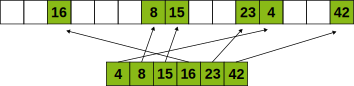
\includegraphics{index_files/mediabag/books/w-python-numpy-grundlagen/skript/../skript/00-bilder/data_memory_list.pdf}

}

\caption{\label{fig-python_memory}Speicherung von Daten in nativem
Python}

\end{figure}%

Dagegen werden NumPy Arrays und Matritzen zusammenhängend gespeichert,
was einen effizienteren Datenaufruf ermöglicht.

\begin{figure}[H]

\centering{

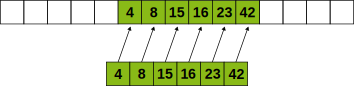
\includegraphics{index_files/mediabag/books/w-python-numpy-grundlagen/skript/../skript/00-bilder/data_memory_numpy.pdf}

}

\caption{\label{fig-numpy_memory}Speicherung von Daten bei Numpy}

\end{figure}%

Dies bedeutet aber auch, dass es eine Erweiterung der Liste deutlich
schneller ist als eine Erweiterung von Arrays oder Matrizen. Bei Listen
kann jeder freie Platz genutzt werden, während Arrays und Matrizen an
einen neuen Ort im Speicher kopiert werden müssen.

\end{tcolorbox}

\section{Einbinden des Pakets}\label{einbinden-des-pakets}

NumPy wird über folgende Zeile eingebunden. Dabei hat sich global der
Standard entwickelt, als Alias \texttt{np} zu verwenden.

\begin{Shaded}
\begin{Highlighting}[]
\ImportTok{import}\NormalTok{ numpy }\ImportTok{as}\NormalTok{ np}
\end{Highlighting}
\end{Shaded}

\section{Referenzen}\label{referenzen}

Sämtliche hier vorgestellten Funktionen lassen sich in der (englischen)
NumPy-Dokumentation nachschlagen:
\href{https://numpy.org/doc/}{Dokumentation}

\chapter{Erstellen von NumPy arrays}\label{erstellen-von-numpy-arrays}

Typischerweise werden in Python Vektoren durch Listen und Matrizen durch
geschachtelte Listen ausgedrückt. Beispielsweise würde man den Vektor

\begin{figure}

\begin{minipage}{0.33\linewidth}
\[
(1, 2, 3, 4, 5, 6) 
\]\end{minipage}%
%
\begin{minipage}{0.33\linewidth}
und die Matrix\end{minipage}%
%
\begin{minipage}{0.33\linewidth}
\[
\begin{pmatrix}
1 & 2 & 3\\
4 & 5 & 6
\end{pmatrix}
\]\end{minipage}%

\end{figure}%

nativ in Python so erstellen:

\begin{Shaded}
\begin{Highlighting}[]
\NormalTok{liste }\OperatorTok{=}\NormalTok{ [}\DecValTok{1}\NormalTok{, }\DecValTok{2}\NormalTok{, }\DecValTok{3}\NormalTok{, }\DecValTok{4}\NormalTok{, }\DecValTok{5}\NormalTok{, }\DecValTok{6}\NormalTok{]}

\NormalTok{matrix }\OperatorTok{=}\NormalTok{ [[}\DecValTok{1}\NormalTok{, }\DecValTok{2}\NormalTok{, }\DecValTok{3}\NormalTok{], [}\DecValTok{4}\NormalTok{, }\DecValTok{5}\NormalTok{, }\DecValTok{6}\NormalTok{]]}

\BuiltInTok{print}\NormalTok{(liste)}
\BuiltInTok{print}\NormalTok{(matrix)}
\end{Highlighting}
\end{Shaded}

\begin{verbatim}
[1, 2, 3, 4, 5, 6]
[[1, 2, 3], [4, 5, 6]]
\end{verbatim}

Möchte man jetzt NumPy Arrays verwenden benutzt man den Befehl
\texttt{np.array()}.

\begin{Shaded}
\begin{Highlighting}[]
\NormalTok{liste }\OperatorTok{=}\NormalTok{ np.array([}\DecValTok{1}\NormalTok{, }\DecValTok{2}\NormalTok{, }\DecValTok{3}\NormalTok{, }\DecValTok{4}\NormalTok{, }\DecValTok{5}\NormalTok{, }\DecValTok{6}\NormalTok{])}

\NormalTok{matrix }\OperatorTok{=}\NormalTok{ np.array([[}\DecValTok{1}\NormalTok{, }\DecValTok{2}\NormalTok{, }\DecValTok{3}\NormalTok{], [}\DecValTok{4}\NormalTok{, }\DecValTok{5}\NormalTok{, }\DecValTok{6}\NormalTok{]])}

\BuiltInTok{print}\NormalTok{(liste)}
\BuiltInTok{print}\NormalTok{(matrix)}
\end{Highlighting}
\end{Shaded}

\begin{verbatim}
[1 2 3 4 5 6]
[[1 2 3]
 [4 5 6]]
\end{verbatim}

Betrachtet man die Ausgaben der \texttt{print()} Befehle fallen zwei
Sachen auf. Zum einen fallen die Kommata weg und zum anderen wird die
Matrix passend ausgegeben.

Es gibt auch die Möglichkeit, höherdimensionale Arrays zu erstellen.
Dabei wird eine neue Ebene der Verschachtelung benutzt. Im folgenden
Beispiel wird eine drei-dimensionale Matrix erstellt.

\begin{Shaded}
\begin{Highlighting}[]
\NormalTok{matrix\_3d }\OperatorTok{=}\NormalTok{ np.array([[[}\DecValTok{1}\NormalTok{, }\DecValTok{2}\NormalTok{, }\DecValTok{3}\NormalTok{], [}\DecValTok{4}\NormalTok{, }\DecValTok{5}\NormalTok{, }\DecValTok{6}\NormalTok{]], [[}\DecValTok{7}\NormalTok{, }\DecValTok{8}\NormalTok{, }\DecValTok{9}\NormalTok{], [}\DecValTok{10}\NormalTok{, }\DecValTok{11}\NormalTok{, }\DecValTok{12}\NormalTok{]]])}
\end{Highlighting}
\end{Shaded}

Es gilt als ``good practice'' Arrays immer zu initialisieren. Dafür
bietet NumPy drei Funktionen um vorinitialisierte Arrays zu erzeugen.
Alternativ können Arrays auch mit festgesetzten Werten initialisiert
werden. Dafür kann entweder die Funktion \texttt{np.zeros()}verwendet
werden die alle Werte auf 0 setzt, oder aber \texttt{np.ones()}welche
alle Werte mit 1 initialisiert. Der Funktion wird die Form im Format
\texttt{{[}Reihen,Spalten{]}} übergeben. Möchte man alle Einträge auf
einen spezifischen Wert setzen, kann man den Befehl \texttt{np.full()}
benutzen.

\begin{Shaded}
\begin{Highlighting}[]
\NormalTok{np.zeros([}\DecValTok{2}\NormalTok{,}\DecValTok{3}\NormalTok{])}
\end{Highlighting}
\end{Shaded}

\begin{verbatim}
array([[0., 0., 0.],
       [0., 0., 0.]])
\end{verbatim}

\begin{Shaded}
\begin{Highlighting}[]
\NormalTok{np.ones([}\DecValTok{2}\NormalTok{,}\DecValTok{3}\NormalTok{])}
\end{Highlighting}
\end{Shaded}

\begin{verbatim}
array([[1., 1., 1.],
       [1., 1., 1.]])
\end{verbatim}

\begin{Shaded}
\begin{Highlighting}[]
\NormalTok{np.full([}\DecValTok{2}\NormalTok{,}\DecValTok{3}\NormalTok{],}\DecValTok{7}\NormalTok{)}
\end{Highlighting}
\end{Shaded}

\begin{verbatim}
array([[7, 7, 7],
       [7, 7, 7]])
\end{verbatim}

\begin{tcolorbox}[enhanced jigsaw, breakable, opacityback=0, left=2mm, coltitle=black, leftrule=.75mm, colframe=quarto-callout-tip-color-frame, opacitybacktitle=0.6, toprule=.15mm, bottomtitle=1mm, titlerule=0mm, toptitle=1mm, title=\textcolor{quarto-callout-tip-color}{\faLightbulb}\hspace{0.5em}{Wie könnte man auch Arrays die mit einer Zahl x gefühlt sind erstellen?}, colbacktitle=quarto-callout-tip-color!10!white, arc=.35mm, bottomrule=.15mm, rightrule=.15mm, colback=white]

Der Trick beseht hierbei ein Array mit \texttt{np.ones()} zu
initialisiere und dieses Array dann mit der Zahl x zu multiplizieren. Im
folgenden Beispiel ist \texttt{x\ =\ 5}

\begin{Shaded}
\begin{Highlighting}[]
\NormalTok{np.ones([}\DecValTok{2}\NormalTok{,}\DecValTok{3}\NormalTok{]) }\OperatorTok{*} \DecValTok{5}
\end{Highlighting}
\end{Shaded}

\begin{verbatim}
array([[5., 5., 5.],
       [5., 5., 5.]])
\end{verbatim}

\end{tcolorbox}

Möchte man zum Beispiel für eine Achse in einem Plot einen Vektor mit
gleichmäßig verteilten Werten erstellen, bieten sich in NumPy zwei
Möglichkeiten. Mit den Befehlen
\texttt{np.linspace(Start,Stop,\#Anzahl\ Werte)} und
\texttt{np.arrange(Start,Stop,Abstand\ zwischen\ Werten)} können solche
Arrays erstellt werden.

\begin{Shaded}
\begin{Highlighting}[]
\NormalTok{np.linspace(}\DecValTok{0}\NormalTok{,}\DecValTok{1}\NormalTok{,}\DecValTok{11}\NormalTok{)}
\end{Highlighting}
\end{Shaded}

\begin{verbatim}
array([0. , 0.1, 0.2, 0.3, 0.4, 0.5, 0.6, 0.7, 0.8, 0.9, 1. ])
\end{verbatim}

\begin{Shaded}
\begin{Highlighting}[]
\NormalTok{np.arange(}\DecValTok{0}\NormalTok{,}\DecValTok{10}\NormalTok{,}\DecValTok{2}\NormalTok{)}
\end{Highlighting}
\end{Shaded}

\begin{verbatim}
array([0, 2, 4, 6, 8])
\end{verbatim}

\begin{tcolorbox}[enhanced jigsaw, breakable, opacityback=0, left=2mm, coltitle=black, leftrule=.75mm, colframe=quarto-callout-tip-color-frame, opacitybacktitle=0.6, toprule=.15mm, bottomtitle=1mm, titlerule=0mm, toptitle=1mm, title=\textcolor{quarto-callout-tip-color}{\faLightbulb}\hspace{0.5em}{Zwischenübung: Array Erstellung}, colbacktitle=quarto-callout-tip-color!10!white, arc=.35mm, bottomrule=.15mm, rightrule=.15mm, colback=white]

Erstellen Sie jeweils ein NumPy-Array, mit dem folgenden Inhalt:

\begin{enumerate}
\def\labelenumi{\arabic{enumi}.}
\tightlist
\item
  mit den Werten 1, 7, 42, 99
\item
  zehn mal die Zahl 5
\item
  mit den Zahlen von 35 \textbf{bis einschließlich} 50
\item
  mit allen geraden Zahlen von 20 \textbf{bis einschließlich} 40
\item
  eine Matrix mit 5 Spalten und 4 Reihen mit dem Wert 4 an jeder Stelle
\item
  mit 10 Werten die gleichmäßig zwischen 22 und einschlieslich 40
  verteilt sind
\end{enumerate}

\begin{tcolorbox}[enhanced jigsaw, breakable, opacityback=0, left=2mm, coltitle=black, leftrule=.75mm, colframe=quarto-callout-caution-color-frame, opacitybacktitle=0.6, toprule=.15mm, bottomtitle=1mm, titlerule=0mm, toptitle=1mm, title={Lösung}, colbacktitle=quarto-callout-caution-color!10!white, arc=.35mm, bottomrule=.15mm, rightrule=.15mm, colback=white]

\begin{Shaded}
\begin{Highlighting}[]
\CommentTok{\# 1. }
\BuiltInTok{print}\NormalTok{(np.array([}\DecValTok{1}\NormalTok{, }\DecValTok{7}\NormalTok{, }\DecValTok{42}\NormalTok{, }\DecValTok{99}\NormalTok{]))}
\end{Highlighting}
\end{Shaded}

\begin{verbatim}
[ 1  7 42 99]
\end{verbatim}

\begin{Shaded}
\begin{Highlighting}[]
\CommentTok{\# 2. }
\BuiltInTok{print}\NormalTok{(np.full(}\DecValTok{10}\NormalTok{,}\DecValTok{5}\NormalTok{))}
\end{Highlighting}
\end{Shaded}

\begin{verbatim}
[5 5 5 5 5 5 5 5 5 5]
\end{verbatim}

\begin{Shaded}
\begin{Highlighting}[]
\CommentTok{\# 3. }
\BuiltInTok{print}\NormalTok{(np.arange(}\DecValTok{35}\NormalTok{, }\DecValTok{51}\NormalTok{))}
\end{Highlighting}
\end{Shaded}

\begin{verbatim}
[35 36 37 38 39 40 41 42 43 44 45 46 47 48 49 50]
\end{verbatim}

\begin{Shaded}
\begin{Highlighting}[]
\CommentTok{\# 4. }
\BuiltInTok{print}\NormalTok{(np.arange(}\DecValTok{20}\NormalTok{, }\DecValTok{41}\NormalTok{, }\DecValTok{2}\NormalTok{))}
\end{Highlighting}
\end{Shaded}

\begin{verbatim}
[20 22 24 26 28 30 32 34 36 38 40]
\end{verbatim}

\begin{Shaded}
\begin{Highlighting}[]
\CommentTok{\# 5. }
\BuiltInTok{print}\NormalTok{(np.full([}\DecValTok{4}\NormalTok{,}\DecValTok{5}\NormalTok{],}\DecValTok{4}\NormalTok{))}
\end{Highlighting}
\end{Shaded}

\begin{verbatim}
[[4 4 4 4 4]
 [4 4 4 4 4]
 [4 4 4 4 4]
 [4 4 4 4 4]]
\end{verbatim}

\begin{Shaded}
\begin{Highlighting}[]
\CommentTok{\# 6. }
\BuiltInTok{print}\NormalTok{(np.linspace(}\DecValTok{22}\NormalTok{, }\DecValTok{40}\NormalTok{, }\DecValTok{10}\NormalTok{))}
\end{Highlighting}
\end{Shaded}

\begin{verbatim}
[22. 24. 26. 28. 30. 32. 34. 36. 38. 40.]
\end{verbatim}

\end{tcolorbox}

\end{tcolorbox}

\chapter{Größe, Struktur und Typ}\label{gruxf6uxdfe-struktur-und-typ}

Wenn man sich nicht mehr sicher ist, welche Struktur oder Form ein Array
hat oder oder diese Größen zum Beispiel für Schleifen nutzen möchte,
bietet NumPy folgende Funktionen für das Auslesen dieser Größen an.

\begin{Shaded}
\begin{Highlighting}[]
\NormalTok{matrix }\OperatorTok{=}\NormalTok{ np.array([[}\DecValTok{1}\NormalTok{, }\DecValTok{2}\NormalTok{, }\DecValTok{3}\NormalTok{], [}\DecValTok{4}\NormalTok{, }\DecValTok{5}\NormalTok{, }\DecValTok{6}\NormalTok{]])}
\end{Highlighting}
\end{Shaded}

\texttt{np.shape()} gibt die Längen der einzelnen Dimension in Form
einer Liste zurück.

\begin{Shaded}
\begin{Highlighting}[]
\NormalTok{np.shape(matrix)}
\end{Highlighting}
\end{Shaded}

\begin{verbatim}
(2, 3)
\end{verbatim}

Die native Python Funktion \texttt{len()} gibt dagegen nur die Länge der
ersten Dimension, also die Anzahl der Elemente in den äußeren Klammern
wieder. Im obrigen Beispiel würde \texttt{len()} also die beiden Listen
\texttt{{[}1,\ 2,\ 3{]}} und \texttt{{[}4,\ 5,\ 6{]}} sehen.

\begin{Shaded}
\begin{Highlighting}[]
\BuiltInTok{len}\NormalTok{(matrix)}
\end{Highlighting}
\end{Shaded}

\begin{verbatim}
2
\end{verbatim}

Die Funktion \texttt{np.ndym()} gibt im Gegensatz zu \texttt{np.shape()}
nur die Anzahl der Dimensionen zurück.

\begin{Shaded}
\begin{Highlighting}[]
\NormalTok{np.ndim(matrix)}
\end{Highlighting}
\end{Shaded}

\begin{verbatim}
2
\end{verbatim}

\begin{tcolorbox}[enhanced jigsaw, breakable, opacityback=0, left=2mm, coltitle=black, leftrule=.75mm, colframe=quarto-callout-tip-color-frame, opacitybacktitle=0.6, toprule=.15mm, bottomtitle=1mm, titlerule=0mm, toptitle=1mm, title=\textcolor{quarto-callout-tip-color}{\faLightbulb}\hspace{0.5em}{Die Ausgabe von \texttt{np.ndim()} kann mit \texttt{np.shape()}und einer
nativen Python Funktion erreicht werden. Wie?}, colbacktitle=quarto-callout-tip-color!10!white, arc=.35mm, bottomrule=.15mm, rightrule=.15mm, colback=white]

\texttt{np.ndim()} gibt die Länge der Liste von \texttt{np.shape()} aus

\begin{Shaded}
\begin{Highlighting}[]
\BuiltInTok{len}\NormalTok{(np.shape(matrix))}
\end{Highlighting}
\end{Shaded}

\begin{verbatim}
2
\end{verbatim}

\end{tcolorbox}

Möchte man die Anzahl aller Elemente in einem Array ausgeben kann man
die Funktion \texttt{np.size()} benutzen.

\begin{Shaded}
\begin{Highlighting}[]
\NormalTok{np.size(matrix)}
\end{Highlighting}
\end{Shaded}

\begin{verbatim}
6
\end{verbatim}

NumPy Arrays können verschiedene Datentypen beinhalten. Im folgenden
haben wir drei verschiedene Arrays mit einem jeweils anderen Datentyp.

\begin{Shaded}
\begin{Highlighting}[]
\NormalTok{typ\_a }\OperatorTok{=}\NormalTok{ np.array([}\DecValTok{1}\NormalTok{, }\DecValTok{2}\NormalTok{, }\DecValTok{3}\NormalTok{, }\DecValTok{4}\NormalTok{, }\DecValTok{5}\NormalTok{])}
\NormalTok{typ\_b }\OperatorTok{=}\NormalTok{ np.array([}\FloatTok{0.1}\NormalTok{, }\FloatTok{0.2}\NormalTok{, }\FloatTok{0.3}\NormalTok{, }\FloatTok{0.4}\NormalTok{, }\FloatTok{0.5}\NormalTok{])}
\NormalTok{typ\_c }\OperatorTok{=}\NormalTok{ np.array([}\StringTok{"Montag"}\NormalTok{, }\StringTok{"Dienstag"}\NormalTok{, }\StringTok{"Mittwoch"}\NormalTok{])}
\end{Highlighting}
\end{Shaded}

Mit der Methode \texttt{np.dtype} können wir den Datentyp von Arrays
ausgeben lassen. Meist wird dabei der Typ plus eine Zahl ausgegeben,
welche die zum Speichern benötigte Bytezahl angibt. Das Array
\emph{typ\_a} beinhaltet den Datentyp int64, also ganze Zahlen.

\begin{Shaded}
\begin{Highlighting}[]
\BuiltInTok{print}\NormalTok{(typ\_a.dtype)}
\end{Highlighting}
\end{Shaded}

\begin{verbatim}
int64
\end{verbatim}

Das Array \emph{typ\_b} beinhaltet den Datentyp float64, wobei float für
Gleitkommazahlen steht.

\begin{Shaded}
\begin{Highlighting}[]
\BuiltInTok{print}\NormalTok{(typ\_b.dtype)}
\end{Highlighting}
\end{Shaded}

\begin{verbatim}
float64
\end{verbatim}

Das Array \emph{typ\_c} beinhaltet den Datentyp U8, wobei das U für
Unicode steht. Hier wird als Unicodetext gespeichert.

\begin{Shaded}
\begin{Highlighting}[]
\BuiltInTok{print}\NormalTok{(typ\_c.dtype)}
\end{Highlighting}
\end{Shaded}

\begin{verbatim}
<U8
\end{verbatim}

Im folgenden finden Sie eine Tabelle mit den typischen Datentypen, die
sie häufig antreffen.

\begin{longtable}[]{@{}lll@{}}
\caption{Typische Datentypen in
NumPy}\label{tbl-datatypes}\tabularnewline
\toprule\noalign{}
Datentyp & Numpy Name & Beispiele \\
\midrule\noalign{}
\endfirsthead
\toprule\noalign{}
Datentyp & Numpy Name & Beispiele \\
\midrule\noalign{}
\endhead
\bottomrule\noalign{}
\endlastfoot
Wahrheitswert & \texttt{bool} & {[}True, False, True{]} \\
Ganze Zahl & \texttt{int} & {[}-2, 5, -6, 7, 3{]} \\
positive Ganze Zahlen & \texttt{uint} & {[}1, 2, 3, 4, 5{]} \\
Kommazahlen & \texttt{float} & {[}1.3, 7.4, 3.5, 5.5{]} \\
komplexe zahlen & \texttt{complex} & {[}-1 + 9j, 2-77j, 72 + 11j{]} \\
Textzeichen & \texttt{U} & {[}``montag'', ``dienstag''{]} \\
\end{longtable}

\begin{tcolorbox}[enhanced jigsaw, breakable, opacityback=0, left=2mm, coltitle=black, leftrule=.75mm, colframe=quarto-callout-tip-color-frame, opacitybacktitle=0.6, toprule=.15mm, bottomtitle=1mm, titlerule=0mm, toptitle=1mm, title=\textcolor{quarto-callout-tip-color}{\faLightbulb}\hspace{0.5em}{Zwischenübung: Arrayinformationen auslesen}, colbacktitle=quarto-callout-tip-color!10!white, arc=.35mm, bottomrule=.15mm, rightrule=.15mm, colback=white]

Gegeben sei folgende Matrix:

\begin{Shaded}
\begin{Highlighting}[]
\NormalTok{matrix }\OperatorTok{=}\NormalTok{ np.array([[[ }\DecValTok{0}\NormalTok{,  }\DecValTok{1}\NormalTok{,  }\DecValTok{2}\NormalTok{,  }\DecValTok{3}\NormalTok{],}
\NormalTok{                 [ }\DecValTok{4}\NormalTok{,  }\DecValTok{5}\NormalTok{,  }\DecValTok{6}\NormalTok{,  }\DecValTok{7}\NormalTok{],}
\NormalTok{                 [ }\DecValTok{8}\NormalTok{,  }\DecValTok{9}\NormalTok{, }\DecValTok{10}\NormalTok{, }\DecValTok{11}\NormalTok{]],}

\NormalTok{                [[}\DecValTok{12}\NormalTok{, }\DecValTok{13}\NormalTok{, }\DecValTok{14}\NormalTok{, }\DecValTok{15}\NormalTok{],}
\NormalTok{                 [}\DecValTok{16}\NormalTok{, }\DecValTok{17}\NormalTok{, }\DecValTok{18}\NormalTok{, }\DecValTok{19}\NormalTok{],}
\NormalTok{                 [}\DecValTok{20}\NormalTok{, }\DecValTok{21}\NormalTok{, }\DecValTok{22}\NormalTok{, }\DecValTok{23}\NormalTok{]],}

\NormalTok{                [[}\DecValTok{24}\NormalTok{, }\DecValTok{25}\NormalTok{, }\DecValTok{26}\NormalTok{, }\DecValTok{27}\NormalTok{],}
\NormalTok{                 [}\DecValTok{28}\NormalTok{, }\DecValTok{29}\NormalTok{, }\DecValTok{30}\NormalTok{, }\DecValTok{31}\NormalTok{],}
\NormalTok{                 [}\DecValTok{32}\NormalTok{, }\DecValTok{33}\NormalTok{, }\DecValTok{34}\NormalTok{, }\DecValTok{35}\NormalTok{]]])}
\end{Highlighting}
\end{Shaded}

Bestimmen Sie durch anschauen die Anzahl an Dimensionen und die Länge
jeder Dimension. Von welchem Typ ist der Inhalt dieser Matrix?

Überprüfen Sie daraufhin Ihre Ergebnisse in dem Sie die passenden
NumPy-Funktionen anwenden.

\begin{tcolorbox}[enhanced jigsaw, breakable, opacityback=0, left=2mm, coltitle=black, leftrule=.75mm, colframe=quarto-callout-caution-color-frame, opacitybacktitle=0.6, toprule=.15mm, bottomtitle=1mm, titlerule=0mm, toptitle=1mm, title={Lösung}, colbacktitle=quarto-callout-caution-color!10!white, arc=.35mm, bottomrule=.15mm, rightrule=.15mm, colback=white]

\begin{Shaded}
\begin{Highlighting}[]
\NormalTok{matrix }\OperatorTok{=}\NormalTok{ np.array([[[ }\DecValTok{0}\NormalTok{,  }\DecValTok{1}\NormalTok{,  }\DecValTok{2}\NormalTok{,  }\DecValTok{3}\NormalTok{],}
\NormalTok{                 [ }\DecValTok{4}\NormalTok{,  }\DecValTok{5}\NormalTok{,  }\DecValTok{6}\NormalTok{,  }\DecValTok{7}\NormalTok{],}
\NormalTok{                 [ }\DecValTok{8}\NormalTok{,  }\DecValTok{9}\NormalTok{, }\DecValTok{10}\NormalTok{, }\DecValTok{11}\NormalTok{]],}

\NormalTok{                [[}\DecValTok{12}\NormalTok{, }\DecValTok{13}\NormalTok{, }\DecValTok{14}\NormalTok{, }\DecValTok{15}\NormalTok{],}
\NormalTok{                 [}\DecValTok{16}\NormalTok{, }\DecValTok{17}\NormalTok{, }\DecValTok{18}\NormalTok{, }\DecValTok{19}\NormalTok{],}
\NormalTok{                 [}\DecValTok{20}\NormalTok{, }\DecValTok{21}\NormalTok{, }\DecValTok{22}\NormalTok{, }\DecValTok{23}\NormalTok{]],}

\NormalTok{                [[}\DecValTok{24}\NormalTok{, }\DecValTok{25}\NormalTok{, }\DecValTok{26}\NormalTok{, }\DecValTok{27}\NormalTok{],}
\NormalTok{                 [}\DecValTok{28}\NormalTok{, }\DecValTok{29}\NormalTok{, }\DecValTok{30}\NormalTok{, }\DecValTok{31}\NormalTok{],}
\NormalTok{                 [}\DecValTok{32}\NormalTok{, }\DecValTok{33}\NormalTok{, }\DecValTok{34}\NormalTok{, }\DecValTok{35}\NormalTok{]]])}

\NormalTok{anzahl\_dimensionen }\OperatorTok{=}\NormalTok{ np.ndim(matrix)}

\BuiltInTok{print}\NormalTok{(}\StringTok{"Anzahl unterschiedlicher Dimensionen: "}\NormalTok{, anzahl\_dimensionen)}

\NormalTok{laenge\_dimensionen }\OperatorTok{=}\NormalTok{ np.shape(matrix)}

\BuiltInTok{print}\NormalTok{(}\StringTok{"Länge der einzelnen DImensionen: "}\NormalTok{, laenge\_dimensionen)}

\BuiltInTok{print}\NormalTok{(matrix.dtype)}
\end{Highlighting}
\end{Shaded}

\begin{verbatim}
Anzahl unterschiedlicher Dimensionen:  3
Länge der einzelnen DImensionen:  (3, 3, 4)
int64
\end{verbatim}

\end{tcolorbox}

\end{tcolorbox}

\chapter{Rechnen mit Arrays}\label{rechnen-mit-arrays}

\section{Arithmetische Funktionen}\label{arithmetische-funktionen}

Ein großer Vorteil an NumPy ist das Rechnen mit Arrays. Ohne NumPy
müsste man entweder eine \texttt{Schleife} oder aber
\texttt{List\ comprehension} benutzen, um mit sämtlichen Werten in der
Liste zu rechnen. In NumPy fällt diese Unannehmlichkeit weg.

\begin{Shaded}
\begin{Highlighting}[]
\NormalTok{a }\OperatorTok{=}\NormalTok{ np.array([}\DecValTok{1}\NormalTok{, }\DecValTok{2}\NormalTok{, }\DecValTok{3}\NormalTok{, }\DecValTok{4}\NormalTok{, }\DecValTok{5}\NormalTok{])}

\NormalTok{b }\OperatorTok{=}\NormalTok{ np.array([}\DecValTok{9}\NormalTok{, }\DecValTok{8}\NormalTok{, }\DecValTok{7}\NormalTok{, }\DecValTok{6}\NormalTok{, }\DecValTok{5}\NormalTok{])}
\end{Highlighting}
\end{Shaded}

Normale mathematische Operationen, wie die Addition, lassen sich auf
zwei Arten ausdrücken. Entweder über die \texttt{np.add()} Funktion oder
aber simpel über das \texttt{+} Zeichen.

\begin{Shaded}
\begin{Highlighting}[]
\NormalTok{np.add(a,b)}
\end{Highlighting}
\end{Shaded}

\begin{verbatim}
array([10, 10, 10, 10, 10])
\end{verbatim}

\begin{Shaded}
\begin{Highlighting}[]
\NormalTok{a }\OperatorTok{+}\NormalTok{ b}
\end{Highlighting}
\end{Shaded}

\begin{verbatim}
array([10, 10, 10, 10, 10])
\end{verbatim}

Ohne NumPy würde die Operation folgendermaßen aussehen:

\begin{Shaded}
\begin{Highlighting}[]
\NormalTok{ergebnis }\OperatorTok{=}\NormalTok{ np.ones(}\DecValTok{5}\NormalTok{)}
\ControlFlowTok{for}\NormalTok{ i }\KeywordTok{in} \BuiltInTok{range}\NormalTok{(}\BuiltInTok{len}\NormalTok{(a)):}
\NormalTok{    ergebnis[i] }\OperatorTok{=}\NormalTok{ a[i] }\OperatorTok{+}\NormalTok{ b[i]}

\BuiltInTok{print}\NormalTok{(ergebnis)}
\end{Highlighting}
\end{Shaded}

\begin{verbatim}
[10. 10. 10. 10. 10.]
\end{verbatim}

Für die anderen Rechenarten existieren auch Funktionen:
\texttt{np.subtract()}, \texttt{np.multiply()} und \texttt{np.divide()}.

Auch für die anderen höheren Rechenoperationen gibt es ebenfalls
Funktionen:

\begin{itemize}
\tightlist
\item
  \texttt{np.exp(a)}
\item
  \texttt{np.sqrt(a)}
\item
  \texttt{np.power(a,\ 3)}
\item
  \texttt{np.sin(a)}
\item
  \texttt{np.cos(a)}
\item
  \texttt{np.tan(a)}
\item
  \texttt{np.log(a)}
\item
  \texttt{a.dot(b)}
\end{itemize}

\begin{tcolorbox}[enhanced jigsaw, breakable, opacityback=0, left=2mm, coltitle=black, leftrule=.75mm, colframe=quarto-callout-warning-color-frame, opacitybacktitle=0.6, toprule=.15mm, bottomtitle=1mm, titlerule=0mm, toptitle=1mm, title=\textcolor{quarto-callout-warning-color}{\faExclamationTriangle}\hspace{0.5em}{Arbeiten mit Winkelfunktionen}, colbacktitle=quarto-callout-warning-color!10!white, arc=.35mm, bottomrule=.15mm, rightrule=.15mm, colback=white]

Wie auch am Taschenrechner birgt das Arbeiten mit den Winkelfunktionen
(sin, cos, \ldots) die Fehlerquelle, dass man nicht mit Radian-Werten,
sondern mit Grad-Werten arbeitet. Die Winkelfunktionen in numpy erwarten
jedoch Radian-Werte.

Für eine einfache Umrechnung bietet NumPy die Funktionen
\texttt{np.grad2rad()}und \texttt{np.rad2grad()}.

\end{tcolorbox}

\section{Vergleiche}\label{vergleiche}

NumPy-Arrays lassen sich auch miteinander vergleichen. Betrachten wir
die folgenden zwei Arrays:

\begin{Shaded}
\begin{Highlighting}[]
\NormalTok{a }\OperatorTok{=}\NormalTok{ np.array([}\DecValTok{1}\NormalTok{, }\DecValTok{2}\NormalTok{, }\DecValTok{3}\NormalTok{, }\DecValTok{4}\NormalTok{, }\DecValTok{5}\NormalTok{])}

\NormalTok{b }\OperatorTok{=}\NormalTok{ np.array([}\DecValTok{9}\NormalTok{, }\DecValTok{2}\NormalTok{, }\DecValTok{7}\NormalTok{, }\DecValTok{4}\NormalTok{, }\DecValTok{5}\NormalTok{])}
\end{Highlighting}
\end{Shaded}

Möchten wir feststellen, ob diese zwei Arrays identisch sind, können wir
den \texttt{==}-Komparator benutzen. Dieser vergleicht die Arrays
elementweise.

\begin{Shaded}
\begin{Highlighting}[]
\NormalTok{a }\OperatorTok{==}\NormalTok{ b}
\end{Highlighting}
\end{Shaded}

\begin{verbatim}
array([False,  True, False,  True,  True])
\end{verbatim}

Es ist außerdem möglich Arrays mit den \texttt{\textgreater{}}- und
\texttt{\textless{}}-Operatoren zu vergleichen:

\begin{Shaded}
\begin{Highlighting}[]
\NormalTok{a }\OperatorTok{\textless{}}\NormalTok{ b}
\end{Highlighting}
\end{Shaded}

\begin{verbatim}
array([ True, False,  True, False, False])
\end{verbatim}

Möchte man Arrays mit Gleitkommazahlen vergleichen, ist es oftmals
nötig, eine gewisse Toleranz zu benutzen, da bei Rechenoperationen
minimale Rundungsfehler entstehen können.

\begin{Shaded}
\begin{Highlighting}[]
\NormalTok{a }\OperatorTok{=}\NormalTok{ np.array(}\FloatTok{0.1} \OperatorTok{+} \FloatTok{0.2}\NormalTok{)}
\NormalTok{b }\OperatorTok{=}\NormalTok{ np.array(}\FloatTok{0.3}\NormalTok{)}
\NormalTok{a }\OperatorTok{==}\NormalTok{ b}
\end{Highlighting}
\end{Shaded}

\begin{verbatim}
np.False_
\end{verbatim}

Für diesen Fall gibt es eine Vergleichsfunktion
\texttt{np.isclose(a,b,atol)}, wobei \texttt{atol} für die absolute
Toleranz steht. Im folgenden Beispiel wird eine absolute Toleranz von
0,001 verwendet.

\begin{Shaded}
\begin{Highlighting}[]
\NormalTok{a }\OperatorTok{=}\NormalTok{ np.array(}\FloatTok{0.1} \OperatorTok{+} \FloatTok{0.2}\NormalTok{)}
\NormalTok{b }\OperatorTok{=}\NormalTok{ np.array(}\FloatTok{0.3}\NormalTok{)}
\BuiltInTok{print}\NormalTok{(np.isclose(a, b, atol}\OperatorTok{=}\FloatTok{0.001}\NormalTok{))}
\end{Highlighting}
\end{Shaded}

\begin{verbatim}
True
\end{verbatim}

\begin{tcolorbox}[enhanced jigsaw, breakable, opacityback=0, left=2mm, coltitle=black, leftrule=.75mm, colframe=quarto-callout-note-color-frame, opacitybacktitle=0.6, toprule=.15mm, bottomtitle=1mm, titlerule=0mm, toptitle=1mm, title=\textcolor{quarto-callout-note-color}{\faInfo}\hspace{0.5em}{Warum ist 0.1 + 0.2 nicht gleich 0.3?}, colbacktitle=quarto-callout-note-color!10!white, arc=.35mm, bottomrule=.15mm, rightrule=.15mm, colback=white]

Zahlen werden intern als Binärzahlen dargestellt. So wie 1/3 nicht mit
einer endlichen Anzahl an Ziffern korrekt dargestellt werden kann müssen
Zahlen ggf. gerundet werden, um im Binärsystem dargestellt zu werden.

\begin{Shaded}
\begin{Highlighting}[]
\NormalTok{a }\OperatorTok{=} \FloatTok{0.1}
\NormalTok{b }\OperatorTok{=} \FloatTok{0.2}
\BuiltInTok{print}\NormalTok{(a }\OperatorTok{+}\NormalTok{ b)}
\end{Highlighting}
\end{Shaded}

\begin{verbatim}
0.30000000000000004
\end{verbatim}

\end{tcolorbox}

\section{Aggregatfunktionen}\label{aggregatfunktionen}

Für verschiedene Auswertungen benötigen wir Funktionen, wie etwa die
Summen oder die Mittelwert-Funktion. Starten wir mit einem Beispiel
Array a:

\begin{Shaded}
\begin{Highlighting}[]
\NormalTok{a }\OperatorTok{=}\NormalTok{ np.array([}\DecValTok{1}\NormalTok{, }\DecValTok{2}\NormalTok{, }\DecValTok{3}\NormalTok{, }\DecValTok{4}\NormalTok{, }\DecValTok{8}\NormalTok{])}
\end{Highlighting}
\end{Shaded}

Die Summer wird über die Funktion \texttt{np.sum()} berechnet.

\begin{Shaded}
\begin{Highlighting}[]
\NormalTok{np.}\BuiltInTok{sum}\NormalTok{(a)}
\end{Highlighting}
\end{Shaded}

\begin{verbatim}
np.int64(18)
\end{verbatim}

Natürlich lassen sich auch der Minimalwert und der Maximalwert eines
Arrays ermitteln. Die beiden Funktionen lauten \texttt{np.min()}und
\texttt{np.max()}.

\begin{Shaded}
\begin{Highlighting}[]
\NormalTok{np.}\BuiltInTok{min}\NormalTok{(a)}
\end{Highlighting}
\end{Shaded}

\begin{verbatim}
np.int64(1)
\end{verbatim}

Möchte man nicht das Maximum selbst, sondern die Position des Maximums
bestimmen, wird statt \texttt{np.max} die Funktion
\texttt{np.argmax}verwendet.

Für statistische Auswertungen werden häufig die Funktion für den
Mittelwert \texttt{np.mean()}, die Funktion für den Median
\texttt{np.median()}und die Funktion für die Standardabweichung
\texttt{np.std()}verwendet.

\begin{Shaded}
\begin{Highlighting}[]
\NormalTok{np.mean(a)}
\end{Highlighting}
\end{Shaded}

\begin{verbatim}
np.float64(3.6)
\end{verbatim}

\begin{Shaded}
\begin{Highlighting}[]
\NormalTok{np.median(a)}
\end{Highlighting}
\end{Shaded}

\begin{verbatim}
np.float64(3.0)
\end{verbatim}

\begin{Shaded}
\begin{Highlighting}[]
\NormalTok{np.std(a)}
\end{Highlighting}
\end{Shaded}

\begin{verbatim}
np.float64(2.4166091947189146)
\end{verbatim}

\begin{tcolorbox}[enhanced jigsaw, breakable, opacityback=0, left=2mm, coltitle=black, leftrule=.75mm, colframe=quarto-callout-tip-color-frame, opacitybacktitle=0.6, toprule=.15mm, bottomtitle=1mm, titlerule=0mm, toptitle=1mm, title=\textcolor{quarto-callout-tip-color}{\faLightbulb}\hspace{0.5em}{Zwischenübung: Rechnen mit Arrays}, colbacktitle=quarto-callout-tip-color!10!white, arc=.35mm, bottomrule=.15mm, rightrule=.15mm, colback=white]

Gegeben sind zwei eindimensionale Arrays a und b:

a = np.array({[}10, 20, 30, 40, 50, 60, 70, 80, 90, 100{]}) und b =
np.array({[}5, 15, 25, 35, 45, 55, 65, 75, 85, 95{]})

\begin{enumerate}
\def\labelenumi{\arabic{enumi}.}
\tightlist
\item
  Erstellen Sie ein neues Array, das die Sinuswerte der addierten Arrays
  a und b enthält.
\item
  Berechnen Sie die Summe, den Mittelwert und die Standardabweichung der
  Elemente in a.
\item
  Finden Sie den größten und den kleinsten Wert in a und b.
\end{enumerate}

\begin{tcolorbox}[enhanced jigsaw, breakable, opacityback=0, left=2mm, coltitle=black, leftrule=.75mm, colframe=quarto-callout-caution-color-frame, opacitybacktitle=0.6, toprule=.15mm, bottomtitle=1mm, titlerule=0mm, toptitle=1mm, title={Lösung}, colbacktitle=quarto-callout-caution-color!10!white, arc=.35mm, bottomrule=.15mm, rightrule=.15mm, colback=white]

\begin{Shaded}
\begin{Highlighting}[]
\NormalTok{a }\OperatorTok{=}\NormalTok{ np.array([}\DecValTok{10}\NormalTok{, }\DecValTok{20}\NormalTok{, }\DecValTok{30}\NormalTok{, }\DecValTok{40}\NormalTok{, }\DecValTok{50}\NormalTok{, }\DecValTok{60}\NormalTok{, }\DecValTok{70}\NormalTok{, }\DecValTok{80}\NormalTok{, }\DecValTok{90}\NormalTok{, }\DecValTok{100}\NormalTok{])}
\NormalTok{b }\OperatorTok{=}\NormalTok{ np.array([}\DecValTok{5}\NormalTok{, }\DecValTok{15}\NormalTok{, }\DecValTok{25}\NormalTok{, }\DecValTok{35}\NormalTok{, }\DecValTok{45}\NormalTok{, }\DecValTok{55}\NormalTok{, }\DecValTok{65}\NormalTok{, }\DecValTok{75}\NormalTok{, }\DecValTok{85}\NormalTok{, }\DecValTok{95}\NormalTok{])}

\CommentTok{\# 1.}
\NormalTok{sin\_ab }\OperatorTok{=}\NormalTok{ np.sin(a }\OperatorTok{+}\NormalTok{ b)}

\CommentTok{\# 2.}
\NormalTok{sum\_a }\OperatorTok{=}\NormalTok{ np.}\BuiltInTok{sum}\NormalTok{(a)}
\NormalTok{mean\_a }\OperatorTok{=}\NormalTok{ np.mean(a)}
\NormalTok{std\_a }\OperatorTok{=}\NormalTok{ np.std(a)}

\CommentTok{\# 3.}
\NormalTok{max\_a }\OperatorTok{=}\NormalTok{ np.}\BuiltInTok{max}\NormalTok{(a)}
\NormalTok{min\_a }\OperatorTok{=}\NormalTok{ np.}\BuiltInTok{min}\NormalTok{(a)}
\NormalTok{max\_b }\OperatorTok{=}\NormalTok{ np.}\BuiltInTok{max}\NormalTok{(b)}
\NormalTok{min\_b }\OperatorTok{=}\NormalTok{ np.}\BuiltInTok{min}\NormalTok{(b)}
\end{Highlighting}
\end{Shaded}

\end{tcolorbox}

\end{tcolorbox}

\chapter{Slicing}\label{slicing}

\section{Normales Slicing mit
Zahlenwerten}\label{normales-slicing-mit-zahlenwerten}

\begin{figure}[H]

\centering{

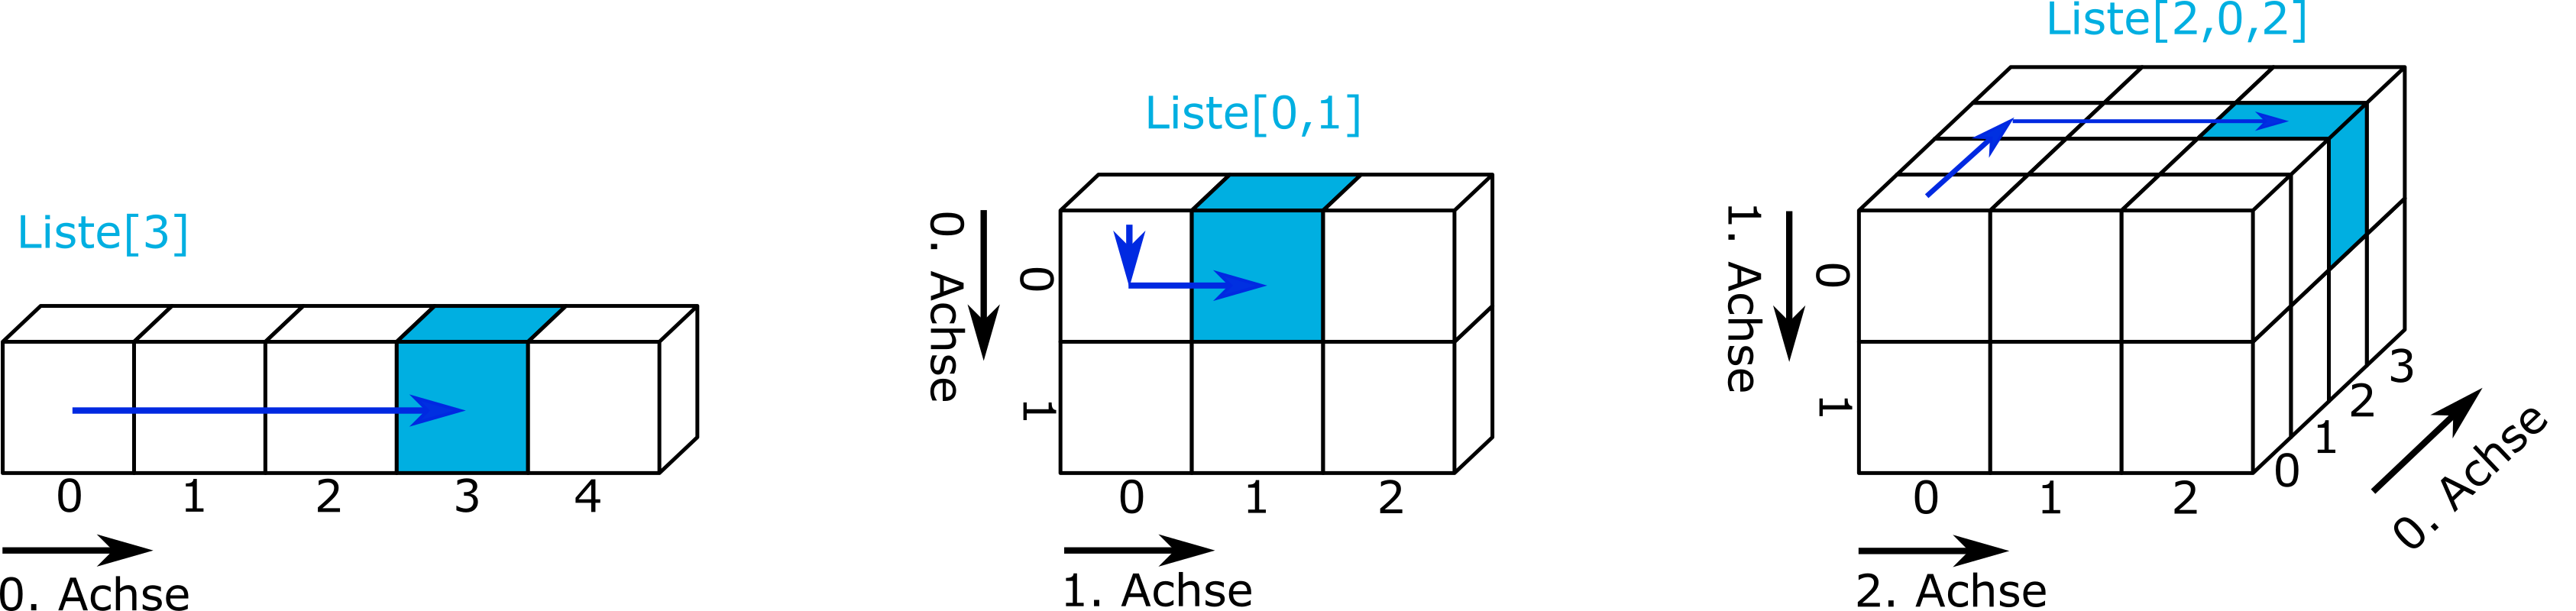
\includegraphics{books/w-python-numpy-grundlagen/skript/../skript/00-bilder/slicing.png}

}

\caption{\label{fig-slicing}Ansprechen der einzelnen Achsen für den
ein-, zwei- und dreidimensionallen Fall inkl. jeweiligem Beispiel}

\end{figure}%

Möchte man jetzt Daten innerhalb eines Arrays auswählen so geschieht das
in der Form:

\begin{enumerate}
\def\labelenumi{\arabic{enumi}.}
\tightlist
\item
  {[}a{]} wobei ein einzelner Wert an Position a ausgegeben wird
\item
  {[}a:b{]} wobei alle Werte von Position a bis Position b-1 ausgegeben
  werden
\item
  {[}a:b:c{]} wobei die Werte von Position a bis Position b-1 mit einer
  Schrittweite von c ausgegeben werden
\end{enumerate}

\begin{Shaded}
\begin{Highlighting}[]
\NormalTok{liste }\OperatorTok{=}\NormalTok{ np.array([}\DecValTok{1}\NormalTok{, }\DecValTok{2}\NormalTok{, }\DecValTok{3}\NormalTok{, }\DecValTok{4}\NormalTok{, }\DecValTok{5}\NormalTok{, }\DecValTok{6}\NormalTok{])}
\end{Highlighting}
\end{Shaded}

\begin{Shaded}
\begin{Highlighting}[]
\CommentTok{\# Auswählen des ersten Elements}
\NormalTok{liste[}\DecValTok{0}\NormalTok{]}
\end{Highlighting}
\end{Shaded}

\begin{verbatim}
np.int64(1)
\end{verbatim}

\begin{Shaded}
\begin{Highlighting}[]
\CommentTok{\# Auswählen des letzen Elements}
\NormalTok{liste[}\OperatorTok{{-}}\DecValTok{1}\NormalTok{]}
\end{Highlighting}
\end{Shaded}

\begin{verbatim}
np.int64(6)
\end{verbatim}

\begin{Shaded}
\begin{Highlighting}[]
\CommentTok{\# Auswählen einer Reihe von Elementen}
\NormalTok{liste[}\DecValTok{1}\NormalTok{:}\DecValTok{4}\NormalTok{]}
\end{Highlighting}
\end{Shaded}

\begin{verbatim}
array([2, 3, 4])
\end{verbatim}

Für zwei-dimensionale Arrays wählt man getrennt durch ein Komma mit
einer zweiten Zahl die zweite Dimension aus.

\begin{Shaded}
\begin{Highlighting}[]
\NormalTok{matrix }\OperatorTok{=}\NormalTok{ np.array([[}\DecValTok{1}\NormalTok{, }\DecValTok{2}\NormalTok{, }\DecValTok{3}\NormalTok{], [}\DecValTok{4}\NormalTok{, }\DecValTok{5}\NormalTok{, }\DecValTok{6}\NormalTok{]])}
\end{Highlighting}
\end{Shaded}

\begin{Shaded}
\begin{Highlighting}[]
\CommentTok{\# Auswählen einer Elements}
\NormalTok{matrix[}\DecValTok{1}\NormalTok{,}\DecValTok{1}\NormalTok{]}
\end{Highlighting}
\end{Shaded}

\begin{verbatim}
np.int64(5)
\end{verbatim}

Für drei-dimensionale Arrays wählt man getrennt durch ein Komma mit
einer weiteren Zahl die dritte Dimension aus. Dabei wird dieses jedoch
an die erste Stelle gesetzt.

\begin{Shaded}
\begin{Highlighting}[]
\NormalTok{matrix\_3d }\OperatorTok{=}\NormalTok{ np.array([[[}\DecValTok{1}\NormalTok{, }\DecValTok{2}\NormalTok{, }\DecValTok{3}\NormalTok{], [}\DecValTok{4}\NormalTok{, }\DecValTok{5}\NormalTok{, }\DecValTok{6}\NormalTok{]], [[}\DecValTok{7}\NormalTok{, }\DecValTok{8}\NormalTok{, }\DecValTok{9}\NormalTok{], [}\DecValTok{10}\NormalTok{, }\DecValTok{11}\NormalTok{, }\DecValTok{12}\NormalTok{]]])}
\BuiltInTok{print}\NormalTok{(matrix\_3d)}
\end{Highlighting}
\end{Shaded}

\begin{verbatim}
[[[ 1  2  3]
  [ 4  5  6]]

 [[ 7  8  9]
  [10 11 12]]]
\end{verbatim}

\begin{Shaded}
\begin{Highlighting}[]
\CommentTok{\# Auswählen eines Elements}
\NormalTok{matrix\_3d[}\DecValTok{1}\NormalTok{,}\DecValTok{0}\NormalTok{,}\DecValTok{2}\NormalTok{]}
\end{Highlighting}
\end{Shaded}

\begin{verbatim}
np.int64(9)
\end{verbatim}

\section{Slicing mit logischen Werten (Boolesche
Masken)}\label{slicing-mit-logischen-werten-boolesche-masken}

Beim logischen Slicing wird eine boolesche Maske verwendet, um bestimmte
Elemente eines Arrays auszuwählen. Die Maske ist ein Array gleicher
Länge wie das Original, das aus \texttt{True} oder \texttt{False} Werten
besteht.

\begin{Shaded}
\begin{Highlighting}[]
\CommentTok{\# Erstellen wir ein Beispiel Array}
\NormalTok{a }\OperatorTok{=}\NormalTok{ np.array([}\DecValTok{1}\NormalTok{, }\DecValTok{2}\NormalTok{, }\DecValTok{3}\NormalTok{, }\DecValTok{4}\NormalTok{, }\DecValTok{5}\NormalTok{, }\DecValTok{6}\NormalTok{])}

\CommentTok{\# Erstellen der Maske}
\NormalTok{maske }\OperatorTok{=}\NormalTok{ a }\OperatorTok{\textgreater{}} \DecValTok{3}

\BuiltInTok{print}\NormalTok{(maske)}
\end{Highlighting}
\end{Shaded}

\begin{verbatim}
[False False False  True  True  True]
\end{verbatim}

Wir erhalten also ein Array mit boolschen Werten. Verwenden wir diese
Maske nun zum slicen, erhalten wir alle Werte an den Stellen, an denen
die Maske den Wert \texttt{True} besitzt.

\begin{Shaded}
\begin{Highlighting}[]
\CommentTok{\# Anwenden der Maske}
\BuiltInTok{print}\NormalTok{(a[maske])}
\end{Highlighting}
\end{Shaded}

\begin{verbatim}
[4 5 6]
\end{verbatim}

\begin{tcolorbox}[enhanced jigsaw, breakable, opacityback=0, left=2mm, coltitle=black, leftrule=.75mm, colframe=quarto-callout-warning-color-frame, opacitybacktitle=0.6, toprule=.15mm, bottomtitle=1mm, titlerule=0mm, toptitle=1mm, title=\textcolor{quarto-callout-warning-color}{\faExclamationTriangle}\hspace{0.5em}{Warning}, colbacktitle=quarto-callout-warning-color!10!white, arc=.35mm, bottomrule=.15mm, rightrule=.15mm, colback=white]

Das Verwenden von booleschen Arrays ist nur im numpy-Modul möglich. Es
ist nicht Möglich dieses Vorgehen auf native Python Listen anzuwenden.
Hier muss durch die Liste iterriert werden.

\begin{Shaded}
\begin{Highlighting}[]
\NormalTok{a }\OperatorTok{=}\NormalTok{ [}\DecValTok{1}\NormalTok{, }\DecValTok{2}\NormalTok{, }\DecValTok{3}\NormalTok{, }\DecValTok{4}\NormalTok{, }\DecValTok{5}\NormalTok{, }\DecValTok{6}\NormalTok{]}
\NormalTok{ergebniss }\OperatorTok{=}\NormalTok{ [x }\ControlFlowTok{for}\NormalTok{ x }\KeywordTok{in}\NormalTok{ a }\ControlFlowTok{if}\NormalTok{ x }\OperatorTok{\textgreater{}} \DecValTok{3}\NormalTok{]}
\BuiltInTok{print}\NormalTok{(ergebniss) }
\end{Highlighting}
\end{Shaded}

\begin{verbatim}
[4, 5, 6]
\end{verbatim}

\end{tcolorbox}

\begin{tcolorbox}[enhanced jigsaw, breakable, opacityback=0, left=2mm, coltitle=black, leftrule=.75mm, colframe=quarto-callout-tip-color-frame, opacitybacktitle=0.6, toprule=.15mm, bottomtitle=1mm, titlerule=0mm, toptitle=1mm, title=\textcolor{quarto-callout-tip-color}{\faLightbulb}\hspace{0.5em}{Zwischenübung: Array-Slicing}, colbacktitle=quarto-callout-tip-color!10!white, arc=.35mm, bottomrule=.15mm, rightrule=.15mm, colback=white]

Wählen Sie die farblich markierten Bereiche aus dem Array ``matrix'' mit
den eben gelernten Möglichkeiten des Array-Slicing aus.


\includegraphics{index_files/mediabag/books/w-python-numpy-grundlagen/skript/../skript/00-bilder/exercise_slicing.pdf}

\begin{Shaded}
\begin{Highlighting}[]
\NormalTok{matrix }\OperatorTok{=}\NormalTok{ np.array([}
\NormalTok{    [}\DecValTok{2}\NormalTok{, }\DecValTok{11}\NormalTok{, }\DecValTok{18}\NormalTok{, }\DecValTok{47}\NormalTok{, }\DecValTok{33}\NormalTok{, }\DecValTok{48}\NormalTok{, }\DecValTok{9}\NormalTok{, }\DecValTok{31}\NormalTok{, }\DecValTok{8}\NormalTok{, }\DecValTok{41}\NormalTok{],}
\NormalTok{    [}\DecValTok{55}\NormalTok{, }\DecValTok{1}\NormalTok{, }\DecValTok{8}\NormalTok{, }\DecValTok{3}\NormalTok{, }\DecValTok{91}\NormalTok{, }\DecValTok{56}\NormalTok{, }\DecValTok{17}\NormalTok{, }\DecValTok{54}\NormalTok{, }\DecValTok{23}\NormalTok{, }\DecValTok{12}\NormalTok{],}
\NormalTok{    [}\DecValTok{19}\NormalTok{, }\DecValTok{99}\NormalTok{, }\DecValTok{56}\NormalTok{, }\DecValTok{72}\NormalTok{, }\DecValTok{6}\NormalTok{, }\DecValTok{13}\NormalTok{, }\DecValTok{34}\NormalTok{, }\DecValTok{16}\NormalTok{, }\DecValTok{77}\NormalTok{, }\DecValTok{56}\NormalTok{],}
\NormalTok{    [}\DecValTok{37}\NormalTok{, }\DecValTok{75}\NormalTok{, }\DecValTok{67}\NormalTok{, }\DecValTok{5}\NormalTok{, }\DecValTok{46}\NormalTok{, }\DecValTok{98}\NormalTok{, }\DecValTok{57}\NormalTok{, }\DecValTok{19}\NormalTok{, }\DecValTok{14}\NormalTok{, }\DecValTok{7}\NormalTok{],}
\NormalTok{    [}\DecValTok{4}\NormalTok{, }\DecValTok{57}\NormalTok{, }\DecValTok{32}\NormalTok{, }\DecValTok{78}\NormalTok{, }\DecValTok{56}\NormalTok{, }\DecValTok{12}\NormalTok{, }\DecValTok{43}\NormalTok{, }\DecValTok{61}\NormalTok{, }\DecValTok{3}\NormalTok{, }\DecValTok{88}\NormalTok{],}
\NormalTok{    [}\DecValTok{96}\NormalTok{, }\DecValTok{16}\NormalTok{, }\DecValTok{92}\NormalTok{, }\DecValTok{18}\NormalTok{, }\DecValTok{50}\NormalTok{, }\DecValTok{90}\NormalTok{, }\DecValTok{35}\NormalTok{, }\DecValTok{15}\NormalTok{, }\DecValTok{36}\NormalTok{, }\DecValTok{97}\NormalTok{],}
\NormalTok{    [}\DecValTok{75}\NormalTok{, }\DecValTok{4}\NormalTok{, }\DecValTok{38}\NormalTok{, }\DecValTok{53}\NormalTok{, }\DecValTok{1}\NormalTok{, }\DecValTok{79}\NormalTok{, }\DecValTok{56}\NormalTok{, }\DecValTok{73}\NormalTok{, }\DecValTok{45}\NormalTok{, }\DecValTok{56}\NormalTok{],}
\NormalTok{    [}\DecValTok{15}\NormalTok{, }\DecValTok{76}\NormalTok{, }\DecValTok{11}\NormalTok{, }\DecValTok{93}\NormalTok{, }\DecValTok{87}\NormalTok{, }\DecValTok{8}\NormalTok{, }\DecValTok{2}\NormalTok{, }\DecValTok{58}\NormalTok{, }\DecValTok{86}\NormalTok{, }\DecValTok{94}\NormalTok{],}
\NormalTok{    [}\DecValTok{51}\NormalTok{, }\DecValTok{14}\NormalTok{, }\DecValTok{60}\NormalTok{, }\DecValTok{57}\NormalTok{, }\DecValTok{74}\NormalTok{, }\DecValTok{42}\NormalTok{, }\DecValTok{59}\NormalTok{, }\DecValTok{71}\NormalTok{, }\DecValTok{88}\NormalTok{, }\DecValTok{52}\NormalTok{],}
\NormalTok{    [}\DecValTok{49}\NormalTok{, }\DecValTok{6}\NormalTok{, }\DecValTok{43}\NormalTok{, }\DecValTok{39}\NormalTok{, }\DecValTok{17}\NormalTok{, }\DecValTok{18}\NormalTok{, }\DecValTok{95}\NormalTok{, }\DecValTok{6}\NormalTok{, }\DecValTok{44}\NormalTok{, }\DecValTok{75}\NormalTok{]}
\NormalTok{])}
\end{Highlighting}
\end{Shaded}

\begin{tcolorbox}[enhanced jigsaw, breakable, opacityback=0, left=2mm, coltitle=black, leftrule=.75mm, colframe=quarto-callout-caution-color-frame, opacitybacktitle=0.6, toprule=.15mm, bottomtitle=1mm, titlerule=0mm, toptitle=1mm, title={Lösung}, colbacktitle=quarto-callout-caution-color!10!white, arc=.35mm, bottomrule=.15mm, rightrule=.15mm, colback=white]

\begin{itemize}
\tightlist
\item
  Rot: matrix{[}1,3{]}
\item
  Grün: matrix{[}4:6,2:6{]}
\item
  Pink: matrix{[}:,7{]}
\item
  Orange: matrix{[}7,:5{]}
\item
  Blau: matrix{[}-1,-1{]}
\end{itemize}

\end{tcolorbox}

\end{tcolorbox}

\chapter{Array Manipulation}\label{array-manipulation}

\section{Ändern der Form}\label{uxe4ndern-der-form}

Durch verschiedene Funktionen lassen sich die Form und die Einträge der
Arrays verändern.

Eine der wichtigsten Array Operationen ist das Transponieren. Dabei
werden Reihen in Spalten und Spalten in Reihe umgewandelt.

\begin{Shaded}
\begin{Highlighting}[]
\NormalTok{matrix }\OperatorTok{=}\NormalTok{ np.array([[}\DecValTok{1}\NormalTok{, }\DecValTok{2}\NormalTok{, }\DecValTok{3}\NormalTok{], [}\DecValTok{4}\NormalTok{, }\DecValTok{5}\NormalTok{, }\DecValTok{6}\NormalTok{]])}
\BuiltInTok{print}\NormalTok{(matrix)}
\end{Highlighting}
\end{Shaded}

\begin{verbatim}
[[1 2 3]
 [4 5 6]]
\end{verbatim}

Transponieren wir dieses Array nun erhalten wir:

\begin{Shaded}
\begin{Highlighting}[]
\BuiltInTok{print}\NormalTok{(np.transpose(matrix))}
\end{Highlighting}
\end{Shaded}

\begin{verbatim}
[[1 4]
 [2 5]
 [3 6]]
\end{verbatim}

Haben wir ein nun diese Matrix und wollen daraus einen Vektor erstellen
so können wir die Funktion \texttt{np.flatten()} benutzen:

\begin{Shaded}
\begin{Highlighting}[]
\NormalTok{vector }\OperatorTok{=}\NormalTok{ matrix.flatten()}
\BuiltInTok{print}\NormalTok{(vector)}
\end{Highlighting}
\end{Shaded}

\begin{verbatim}
[1 2 3 4 5 6]
\end{verbatim}

Um wieder eine zweidimensionale Datenstruktur zu erhalten, benutzen wir
die Funktion \texttt{np.reshape(Ziel,\ Form)}

\begin{Shaded}
\begin{Highlighting}[]
\BuiltInTok{print}\NormalTok{(np.reshape(matrix, [}\DecValTok{3}\NormalTok{, }\DecValTok{2}\NormalTok{]))}
\end{Highlighting}
\end{Shaded}

\begin{verbatim}
[[1 2]
 [3 4]
 [5 6]]
\end{verbatim}

Möchten wir den Inhalt eines bereits bestehenden Arrays erweitern,
verkleinern oder ändern bietet NumPy ebenfalls die passenden Funktionen.

Haben wir ein leeres Array oder wollen wir ein schon volles Array
erweitern benutzen wir die Funktion \texttt{np.append()}. Dabei hängen
wir einen Wert an das bereits bestehende Array an.

\begin{Shaded}
\begin{Highlighting}[]
\NormalTok{liste }\OperatorTok{=}\NormalTok{ np.array([}\DecValTok{1}\NormalTok{, }\DecValTok{2}\NormalTok{, }\DecValTok{3}\NormalTok{, }\DecValTok{4}\NormalTok{, }\DecValTok{5}\NormalTok{, }\DecValTok{6}\NormalTok{])}

\NormalTok{neue\_liste }\OperatorTok{=}\NormalTok{ np.append(liste, }\DecValTok{7}\NormalTok{)}
\BuiltInTok{print}\NormalTok{(neue\_liste)}
\end{Highlighting}
\end{Shaded}

\begin{verbatim}
[1 2 3 4 5 6 7]
\end{verbatim}

Gegebenenfalls ist es nötig einen Wert nicht am Ende, sondern an einer
beliebigen Position im Array einzufügen. Das passende Werkzeug ist hier
die Funktion \texttt{np.insert(Array,\ Position,\ Einschub)}. Im
folgenden Beispiel wird an der dritten Stelle die Zahl 7 eingesetzt.

\begin{Shaded}
\begin{Highlighting}[]
\NormalTok{liste }\OperatorTok{=}\NormalTok{ np.array([}\DecValTok{1}\NormalTok{, }\DecValTok{2}\NormalTok{, }\DecValTok{3}\NormalTok{, }\DecValTok{4}\NormalTok{, }\DecValTok{5}\NormalTok{, }\DecValTok{6}\NormalTok{])}

\NormalTok{neue\_liste }\OperatorTok{=}\NormalTok{ np.insert(liste, }\DecValTok{3}\NormalTok{, }\DecValTok{7}\NormalTok{)}
\BuiltInTok{print}\NormalTok{(neue\_liste)}
\end{Highlighting}
\end{Shaded}

\begin{verbatim}
[1 2 3 7 4 5 6]
\end{verbatim}

Wenn sich neue Elemente einfügen lassen, können natürlich auch Elemente
gelöscht werden. Hierfür wird die Funktion
\texttt{np.delete(Array\ ,\ Position)} benutzt, die ein Array und die
Position der zu löschenden Funktion übergeben bekommt.

\begin{Shaded}
\begin{Highlighting}[]
\NormalTok{liste }\OperatorTok{=}\NormalTok{ np.array([}\DecValTok{1}\NormalTok{, }\DecValTok{2}\NormalTok{, }\DecValTok{3}\NormalTok{, }\DecValTok{4}\NormalTok{, }\DecValTok{5}\NormalTok{, }\DecValTok{6}\NormalTok{])}

\NormalTok{neue\_liste }\OperatorTok{=}\NormalTok{ np.delete(liste, }\DecValTok{3}\NormalTok{)}
\BuiltInTok{print}\NormalTok{(neue\_liste)}
\end{Highlighting}
\end{Shaded}

\begin{verbatim}
[1 2 3 5 6]
\end{verbatim}

Zuletzt wollen wir uns noch die Verbindung zweier Arrays anschauen. Im
folgenden Beispiel wird dabei das Array \texttt{b} an das Array
\texttt{a} mithilfe der Funktion
\texttt{np.concatenate((Array\ a,\ Array\ b))}angehängt.

\begin{Shaded}
\begin{Highlighting}[]
\NormalTok{a }\OperatorTok{=}\NormalTok{ np.array([}\DecValTok{1}\NormalTok{, }\DecValTok{2}\NormalTok{, }\DecValTok{3}\NormalTok{, }\DecValTok{4}\NormalTok{, }\DecValTok{5}\NormalTok{, }\DecValTok{6}\NormalTok{])}
\NormalTok{b }\OperatorTok{=}\NormalTok{ np.array([}\DecValTok{7}\NormalTok{, }\DecValTok{8}\NormalTok{, }\DecValTok{9}\NormalTok{, }\DecValTok{10}\NormalTok{])}

\NormalTok{neue\_liste }\OperatorTok{=}\NormalTok{ np.concatenate((a, b))}
\BuiltInTok{print}\NormalTok{(neue\_liste)}
\end{Highlighting}
\end{Shaded}

\begin{verbatim}
[ 1  2  3  4  5  6  7  8  9 10]
\end{verbatim}

\section{Sortieren von Arrays}\label{sortieren-von-arrays}

NumPy bietet auch die Möglichkeit, Arrays zu sortieren. Im folgenden
Beispiel starten wir mit einem unsortierten Array. Mit der Funktion
\texttt{np.sort()} erhalten wir ein sortiertes Array.

\begin{Shaded}
\begin{Highlighting}[]
\ImportTok{import}\NormalTok{ numpy }\ImportTok{as}\NormalTok{ np}
\NormalTok{unsortiert }\OperatorTok{=}\NormalTok{ np.array([}\DecValTok{4}\NormalTok{, }\DecValTok{2}\NormalTok{, }\DecValTok{1}\NormalTok{, }\DecValTok{6}\NormalTok{, }\DecValTok{3}\NormalTok{, }\DecValTok{5}\NormalTok{])}

\NormalTok{sortiert }\OperatorTok{=}\NormalTok{ np.sort(unsortiert)}

\BuiltInTok{print}\NormalTok{(sortiert)}
\end{Highlighting}
\end{Shaded}

\begin{verbatim}
[1 2 3 4 5 6]
\end{verbatim}

\section{Unterlisten mit einzigartigen
Werten}\label{unterlisten-mit-einzigartigen-werten}

Arbeitet man mit Daten bei denen zum Beispiel Projekte Personalnummern
zugeordnet werden hat man Daten mit einer endlichen Anzahl an
Personalnummern, die jedoch mehrfach vorkommen können wenn diese an mehr
als einem Projekt gleichzeitig arbeiten.

Möchte man nun eine Liste die jede Nummer nur einmal enthält, kann die
Funtkion \texttt{np.unique} verwendet werden.

\begin{Shaded}
\begin{Highlighting}[]
\ImportTok{import}\NormalTok{ numpy }\ImportTok{as}\NormalTok{ np}
\NormalTok{liste\_mit\_dopplungen }\OperatorTok{=}\NormalTok{ np.array([}\DecValTok{4}\NormalTok{, }\DecValTok{1}\NormalTok{, }\DecValTok{1}\NormalTok{, }\DecValTok{6}\NormalTok{, }\DecValTok{3}\NormalTok{, }\DecValTok{4}\NormalTok{, }\DecValTok{7}\NormalTok{, }\DecValTok{3}\NormalTok{, }\DecValTok{3}\NormalTok{])}

\NormalTok{einzigartige\_werte }\OperatorTok{=}\NormalTok{ np.unique(liste\_mit\_dopplungen)}

\BuiltInTok{print}\NormalTok{(einzigartige\_werte)}
\end{Highlighting}
\end{Shaded}

\begin{verbatim}
[1 3 4 6 7]
\end{verbatim}

Setzt man dann noch die Option \texttt{return\_counts=True} kann in
einer zweiten Variable gespeichert werden, wie oft jeder Wert vorkommt.

\begin{Shaded}
\begin{Highlighting}[]
\ImportTok{import}\NormalTok{ numpy }\ImportTok{as}\NormalTok{ np}
\NormalTok{liste\_mit\_dopplungen }\OperatorTok{=}\NormalTok{ np.array([}\DecValTok{4}\NormalTok{, }\DecValTok{1}\NormalTok{, }\DecValTok{1}\NormalTok{, }\DecValTok{6}\NormalTok{, }\DecValTok{3}\NormalTok{, }\DecValTok{4}\NormalTok{, }\DecValTok{7}\NormalTok{, }\DecValTok{3}\NormalTok{, }\DecValTok{3}\NormalTok{])}

\NormalTok{einzigartige\_werte, anzahl }\OperatorTok{=}\NormalTok{ np.unique(liste\_mit\_dopplungen, return\_counts}\OperatorTok{=}\VariableTok{True}\NormalTok{)}

\BuiltInTok{print}\NormalTok{(anzahl)}
\end{Highlighting}
\end{Shaded}

\begin{verbatim}
[2 3 2 1 1]
\end{verbatim}

\begin{tcolorbox}[enhanced jigsaw, breakable, opacityback=0, left=2mm, coltitle=black, leftrule=.75mm, colframe=quarto-callout-tip-color-frame, opacitybacktitle=0.6, toprule=.15mm, bottomtitle=1mm, titlerule=0mm, toptitle=1mm, title=\textcolor{quarto-callout-tip-color}{\faLightbulb}\hspace{0.5em}{Zwischenübung: Arraymanipulation}, colbacktitle=quarto-callout-tip-color!10!white, arc=.35mm, bottomrule=.15mm, rightrule=.15mm, colback=white]

Gegeben ist das folgende zweidimensionale Array matrix:

\begin{Shaded}
\begin{Highlighting}[]
\NormalTok{matrix }\OperatorTok{=}\NormalTok{ np.array([}
\NormalTok{    [}\DecValTok{4}\NormalTok{, }\DecValTok{7}\NormalTok{, }\DecValTok{2}\NormalTok{, }\DecValTok{8}\NormalTok{],}
\NormalTok{    [}\DecValTok{1}\NormalTok{, }\DecValTok{5}\NormalTok{, }\DecValTok{3}\NormalTok{, }\DecValTok{6}\NormalTok{],}
\NormalTok{    [}\DecValTok{9}\NormalTok{, }\DecValTok{2}\NormalTok{, }\DecValTok{4}\NormalTok{, }\DecValTok{7}\NormalTok{]}
\NormalTok{])}
\end{Highlighting}
\end{Shaded}

\begin{enumerate}
\def\labelenumi{\arabic{enumi}.}
\tightlist
\item
  Ändern Sie die Form des Arrays matrix in ein eindimensionales Array.
\item
  Sortieren Sie das eindimensionale Array in aufsteigender Reihenfolge.
\item
  Ändern Sie die Form des sortierten Arrays in ein zweidimensionales
  Array mit 2 Zeilen und 6 Spalten.
\item
  Bestimmen Sie die eindeutigen Elemente im ursprünglichen Array matrix
  und geben Sie diese aus.
\end{enumerate}

\begin{tcolorbox}[enhanced jigsaw, breakable, opacityback=0, left=2mm, coltitle=black, leftrule=.75mm, colframe=quarto-callout-caution-color-frame, opacitybacktitle=0.6, toprule=.15mm, bottomtitle=1mm, titlerule=0mm, toptitle=1mm, title={Lösung}, colbacktitle=quarto-callout-caution-color!10!white, arc=.35mm, bottomrule=.15mm, rightrule=.15mm, colback=white]

\begin{Shaded}
\begin{Highlighting}[]
\NormalTok{matrix }\OperatorTok{=}\NormalTok{ np.array([}
\NormalTok{    [}\DecValTok{4}\NormalTok{, }\DecValTok{7}\NormalTok{, }\DecValTok{2}\NormalTok{, }\DecValTok{8}\NormalTok{],}
\NormalTok{    [}\DecValTok{1}\NormalTok{, }\DecValTok{5}\NormalTok{, }\DecValTok{3}\NormalTok{, }\DecValTok{6}\NormalTok{],}
\NormalTok{    [}\DecValTok{9}\NormalTok{, }\DecValTok{2}\NormalTok{, }\DecValTok{4}\NormalTok{, }\DecValTok{7}\NormalTok{]}
\NormalTok{])}

\CommentTok{\# 1. Ändern der Form in ein eindimensionales Array}
\NormalTok{flat\_array }\OperatorTok{=}\NormalTok{ matrix.flatten()}

\CommentTok{\# 2. Sortieren des eindimensionalen Arrays in aufsteigender Reihenfolge}
\NormalTok{sorted\_array }\OperatorTok{=}\NormalTok{ np.sort(flat\_array)}

\CommentTok{\# 3. Ändern der Form des sortierten Arrays in ein 2x6{-}Array}
\NormalTok{reshaped\_array }\OperatorTok{=}\NormalTok{ sorted\_array.reshape(}\DecValTok{2}\NormalTok{, }\DecValTok{6}\NormalTok{)}

\CommentTok{\# 4. Bestimmen der eindeutigen Elemente im ursprünglichen Array}
\NormalTok{unique\_elements\_original }\OperatorTok{=}\NormalTok{ np.unique(matrix)}
\end{Highlighting}
\end{Shaded}

\end{tcolorbox}

\end{tcolorbox}

\chapter{Lesen und Schreiben von
Dateien}\label{lesen-und-schreiben-von-dateien}

Das Modul numpy stellt Funktionen zum Lesen und Schreiben von
strukturierten Textdateien bereit.

\section{Lesen von Dateien}\label{lesen-von-dateien}

Zum Lesen von strukturierten Textdateien, z.B. im CSV-Format (comma
separated values), kann die \texttt{np.loadtxt()}-Funktion verwendet
werden. Diese bekommt als Argumente den einzulesenden Dateinamen und
weitere Optionen zur Definition der Struktur der Daten. Der Rückgabewert
ist ein (mehrdimensionales) Array.

Im folgenden Beispiel wird die Datei
\href{https://firedynamics.github.io/LectureComputerScience/_downloads/0d1a3bfbc82fa134e08585d6151e9f46/TC01.csv}{TC01.csv}
eingelesen und deren Inhalt graphisch dargestellt. Die erste Zeile der
Datei wird dabei ignoriert, da sie als Kommentar -- eingeleitet durch
das \#-Zeichen -- interpretiert wird.

\begin{Shaded}
\begin{Highlighting}[]
\NormalTok{dateiname }\OperatorTok{=} \StringTok{\textquotesingle{}01{-}daten/TC01.csv\textquotesingle{}}
\NormalTok{daten }\OperatorTok{=}\NormalTok{ np.loadtxt(dateiname)}
\end{Highlighting}
\end{Shaded}

\begin{Shaded}
\begin{Highlighting}[]
\BuiltInTok{print}\NormalTok{(}\StringTok{"Daten:"}\NormalTok{, daten)}
\BuiltInTok{print}\NormalTok{(}\StringTok{"Form:"}\NormalTok{, daten.shape)}
\end{Highlighting}
\end{Shaded}

\begin{verbatim}
Daten: [20.1 20.1 20.1 ... 24.3 24.2 24.2]
Form: (1513,)
\end{verbatim}

\begin{Shaded}
\begin{Highlighting}[]
\NormalTok{plt.plot(daten)}
\NormalTok{plt.xlabel(}\StringTok{\textquotesingle{}Datenindex\textquotesingle{}}\NormalTok{)}
\NormalTok{plt.ylabel(}\StringTok{\textquotesingle{}Temperatur in °C\textquotesingle{}}\NormalTok{)}\OperatorTok{;}
\end{Highlighting}
\end{Shaded}

\includegraphics{books/w-python-numpy-grundlagen/skript/array_read_n_write_files/figure-pdf/cell-5-output-1.pdf}

Standardmäßig erwartet die \texttt{np.loadtxt()}-Funktion Komma
separierte Werte. Werden die Daten durch ein anderes Trennzeichen
getrennt, kann mit der Option \texttt{delimiter\ =\ ""} ein anderes
Trenzeichen ausgewählt werden. Beispielsweise würde der Funktionsaufruf
bei einem Semikolon folgendermaßen aussehen:
\texttt{np.loadtxt(data.txt,\ delimiter\ =\ ";")}

Beginnt die Datei mit den Daten mit Zeilen bezüglich zusätzlichen
Informationen wie Einheiten oder Experimentdaten, können diese mit der
Option \texttt{skiprows=\ \#Reihen}übersprungen werden.

\section{Schreiben von Dateien}\label{schreiben-von-dateien}

Zum Schreiben von Arrays in Dateien, kann die in numpy verfügbare
Funktion \texttt{np.savetxt()} verwendet werden. Dieser müssen
mindestens die zu schreibenden Arrays als auch ein Dateiname übergeben
werden. Darüber hinaus sind zahlreiche Formatierungs- bzw.
Strukturierungsoptionen möglich.

Folgendes Beispiel skaliert die oben eingelesenen Daten und schreib
jeden zehnten Wert in eine Datei. Dabei wird auch ein Kommentar
(\texttt{header}-Argument) am Anfang der Datei erzeugt. Das
Ausgabeformat der Zahlen kann mit dem \texttt{fmt}-Argument angegeben
werden. Das Format ähnelt der Darstellungsweise, welche bei den
formatierten Zeichenketten vorgestellt wurde.

\begin{Shaded}
\begin{Highlighting}[]
\NormalTok{wertebereich }\OperatorTok{=}\NormalTok{ np.}\BuiltInTok{max}\NormalTok{(daten) }\OperatorTok{{-}}\NormalTok{ np.}\BuiltInTok{min}\NormalTok{(daten)}
\NormalTok{daten\_skaliert }\OperatorTok{=}\NormalTok{ ( daten }\OperatorTok{{-}}\NormalTok{ np.}\BuiltInTok{min}\NormalTok{(daten) ) }\OperatorTok{/}\NormalTok{ wertebereich}
\NormalTok{daten\_skaliert }\OperatorTok{=}\NormalTok{ daten\_skaliert[::}\DecValTok{10}\NormalTok{]}
\end{Highlighting}
\end{Shaded}

\begin{Shaded}
\begin{Highlighting}[]
\NormalTok{plt.plot(daten\_skaliert)}
\NormalTok{plt.xlabel(}\StringTok{\textquotesingle{}Datenindex\textquotesingle{}}\NormalTok{)}
\NormalTok{plt.ylabel(}\StringTok{\textquotesingle{}Skalierte Temperatur\textquotesingle{}}\NormalTok{)}\OperatorTok{;}
\end{Highlighting}
\end{Shaded}

\includegraphics{books/w-python-numpy-grundlagen/skript/array_read_n_write_files/figure-pdf/cell-7-output-1.pdf}

Beim Schreiben der Datei wird ein mehrzeiliger Kommentar mithilfe des
Zeilenumbruchzeichens \texttt{\textbackslash{}n} definiert. Die Ausgabe
der Gleitkommazahlen wird mit \texttt{\%5.2f} formatiert, was 5 Stellen
insgesamt und zwei Nachkommastellen entspricht.

\begin{Shaded}
\begin{Highlighting}[]
\CommentTok{\# Zuweisung ist auf mehrere Zeilen aufgeteilt, aufgrund der }
\CommentTok{\# schmalen Darstellung im Skript}
\NormalTok{kommentar }\OperatorTok{=} \SpecialStringTok{f\textquotesingle{}Daten aus }\SpecialCharTok{\{}\NormalTok{dateiname}\SpecialCharTok{\}}\SpecialStringTok{ skaliert auf den Bereich \textquotesingle{}} \OperatorTok{+} \OperatorTok{\textbackslash{}}
             \StringTok{\textquotesingle{}0 bis 1 }\CharTok{\textbackslash{}n}\StringTok{originales Min / Max:\textquotesingle{}} \OperatorTok{+} \OperatorTok{\textbackslash{}}
            \SpecialStringTok{f\textquotesingle{}}\SpecialCharTok{\{}\NormalTok{np}\SpecialCharTok{.}\BuiltInTok{min}\NormalTok{(daten)}\SpecialCharTok{\}}\SpecialStringTok{/}\SpecialCharTok{\{}\NormalTok{np}\SpecialCharTok{.}\BuiltInTok{max}\NormalTok{(daten)}\SpecialCharTok{\}}\SpecialStringTok{\textquotesingle{}}
\NormalTok{neu\_dateiname }\OperatorTok{=} \StringTok{\textquotesingle{}01{-}daten/TC01\_skaliert.csv\textquotesingle{}}

\NormalTok{np.savetxt(neu\_dateiname, daten\_skaliert, }
\NormalTok{           header}\OperatorTok{=}\NormalTok{kommentar, fmt}\OperatorTok{=}\StringTok{\textquotesingle{}}\SpecialCharTok{\%5.2f}\StringTok{\textquotesingle{}}\NormalTok{)}
\end{Highlighting}
\end{Shaded}

Zum Veranschaulichen werden die ersten Zeilen der neuen Datei
ausgegeben.

\begin{Shaded}
\begin{Highlighting}[]
\CommentTok{\# Einlesen der ersten Zeilen der neu erstellten Datei}
\NormalTok{datei }\OperatorTok{=} \BuiltInTok{open}\NormalTok{(neu\_dateiname, }\StringTok{\textquotesingle{}r\textquotesingle{}}\NormalTok{)}
\ControlFlowTok{for}\NormalTok{ i }\KeywordTok{in} \BuiltInTok{range}\NormalTok{(}\DecValTok{10}\NormalTok{):}
    \BuiltInTok{print}\NormalTok{( datei.readline() , end}\OperatorTok{=}\StringTok{\textquotesingle{}\textquotesingle{}}\NormalTok{)}
\NormalTok{datei.close()}
\end{Highlighting}
\end{Shaded}

\begin{verbatim}
# Daten aus 01-daten/TC01.csv skaliert auf den Bereich 0 bis 1 
# originales Min / Max:20.1/31.1
 0.00
 0.00
 0.00
 0.01
 0.01
 0.01
 0.01
 0.01
\end{verbatim}

\chapter{Arbeiten mit Bildern}\label{arbeiten-mit-bildern}

Bilder werden digital als Matrizen gespeichert. Dabei werden pro Pixel
drei Farbwerte (rot, grün, blau) gespeichert. Aus diesen drei Farbwerten
(Wert 0-255) werden dann alle gewünschten Farben zusammengestellt.

\begin{figure}[H]

\centering{

\includegraphics{index_files/mediabag/books/w-python-numpy-grundlagen/skript/../skript/00-bilder/pixel_mona_lisa_split.pdf}

}

\caption{\label{fig-pixel_colors}Ein hochaufgelöstes Bild besteht aus
sehr vielen Pixeln. Jedes Pixel enthät 3 Farbwerte, einen für die Fabre
Grün, einen für Blau und einen für Rot.}

\end{figure}%

Aufgrund der digitalen Darstellung von Bildern lassen sich diese mit den
Werkzeugen von NumPy leicht bearbeiten. Wir verwenden für folgendes
Beispiel als Bild die Monas Lisa. Das Bild ist unter folgendem
\href{https://upload.wikimedia.org/wikipedia/commons/thumb/6/6a/Mona_Lisa.jpg/677px-Mona_Lisa.jpg}{Link}
zu finden.

Importieren wir dieses Bild nun mit der Funktion \texttt{imread()}aus
dem matplotlib-package, sehen wir das es um ein dreidimensionales numpy
Array handelt.

\begin{Shaded}
\begin{Highlighting}[]
\ImportTok{import}\NormalTok{ matplotlib.pyplot }\ImportTok{as}\NormalTok{ plt}

\NormalTok{data }\OperatorTok{=}\NormalTok{ plt.imread(}\StringTok{"00{-}bilder/mona\_lisa.jpg"}\NormalTok{)}
\BuiltInTok{print}\NormalTok{(}\StringTok{"Form:"}\NormalTok{, data.shape)}
\end{Highlighting}
\end{Shaded}

\begin{verbatim}
Form: (1024, 677, 3)
\end{verbatim}

Schauen wir uns einmal mit der \texttt{print()}-Funktion einen
Ausschnitt dieser Daten an.

\begin{Shaded}
\begin{Highlighting}[]
\BuiltInTok{print}\NormalTok{(data)}
\end{Highlighting}
\end{Shaded}

\begin{verbatim}
[[[ 68  62  38]
  [ 88  82  56]
  [ 92  87  55]
  ...
  [ 54  97  44]
  [ 68 110  60]
  [ 69 111  63]]

 [[ 65  59  33]
  [ 68  63  34]
  [ 83  78  46]
  ...
  [ 66 103  51]
  [ 66 103  52]
  [ 66 102  56]]

 [[ 97  90  62]
  [ 87  80  51]
  [ 78  72  38]
  ...
  [ 79 106  53]
  [ 62  89  38]
  [ 62  88  41]]

 ...

 [[ 25  14  18]
  [ 21  10  14]
  [ 20   9  13]
  ...
  [ 11   5   9]
  [ 11   5   9]
  [ 10   4   8]]

 [[ 23  12  16]
  [ 23  12  16]
  [ 21  10  14]
  ...
  [ 11   5   9]
  [ 11   5   9]
  [ 10   4   8]]

 [[ 22  11  15]
  [ 26  15  19]
  [ 24  13  17]
  ...
  [ 11   5   9]
  [ 10   4   8]
  [  9   3   7]]]
\end{verbatim}

Mit der Funktion \texttt{plt.imshow} kann das Bild in Echtfarben
dargestellt werden. Dies funktioniert, da die Funktion die einzelnen
Ebenen, hier der letzte Index, des Datensatzes als Farbinformationen
(rot, grün, blau) interpretiert. Wäre noch eine vierte Ebene dabei,
würde sie als individueller Transparenzwert verwendet worden.

\begin{Shaded}
\begin{Highlighting}[]
\NormalTok{plt.imshow(data)}
\end{Highlighting}
\end{Shaded}

\includegraphics{books/w-python-numpy-grundlagen/skript/array_images_files/figure-pdf/cell-5-output-1.pdf}

Natürlich können auch die einzelnen Farbebenen individuell betrachtet
werden. Dazu wird der letzte Index festgehalten. Hier betrachten wir nur
den reten Anteil des Bildes. Stellen wir ein einfaches Array dar, werden
die Daten in schwarz-weiß ausgegeben. Mit Hilfe der Option
\texttt{cmap=\textquotesingle{}Reds\textquotesingle{}} können wir die
Farbskala anpassen.

\begin{Shaded}
\begin{Highlighting}[]
\CommentTok{\# Als Farbskale wird die Rotskala }
\CommentTok{\# verwendet \textquotesingle{}Reds\textquotesingle{}}
\NormalTok{plt.imshow( data[:,:,}\DecValTok{0}\NormalTok{], cmap}\OperatorTok{=}\StringTok{\textquotesingle{}Reds\textquotesingle{}}\NormalTok{ )}
\NormalTok{plt.colorbar()}
\NormalTok{plt.show()}
\end{Highlighting}
\end{Shaded}

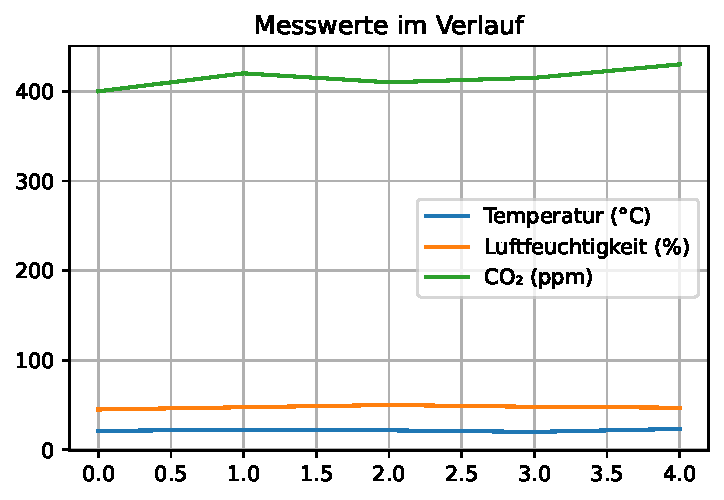
\includegraphics{books/w-python-numpy-grundlagen/skript/array_images_files/figure-pdf/cell-6-output-1.pdf}

Da die Bilddaten als Arrays gespeichert sind, sind viele der möglichen
Optionen, z.B. zur Teilauswahl oder Operationen, verfügbar. Das untere
Beispiel zeigt einen Ausschnitt im Rotkanal des Bildes.

\begin{Shaded}
\begin{Highlighting}[]
\NormalTok{bereich }\OperatorTok{=}\NormalTok{ np.array(data[}\DecValTok{450}\NormalTok{:}\DecValTok{500}\NormalTok{, }\DecValTok{550}\NormalTok{:}\DecValTok{600}\NormalTok{,}\DecValTok{0}\NormalTok{], dtype}\OperatorTok{=}\BuiltInTok{float}\NormalTok{)}
\NormalTok{plt.imshow( bereich, cmap}\OperatorTok{=}\StringTok{"Greys"}\NormalTok{ )}
\NormalTok{plt.colorbar()}
\end{Highlighting}
\end{Shaded}

\includegraphics{books/w-python-numpy-grundlagen/skript/array_images_files/figure-pdf/cell-7-output-1.pdf}

Betrachten wir nun eine komplexere Operation an Bilddaten, den
\href{https://de.wikipedia.org/wiki/Laplace-Operator}{Laplace-Operator}.
Er kann genutzt werden um Ränder von Objekten zu identifizieren. Dazu
wird für jeden Bildpunkt \(B_{i,j}\) -- außer an den Rändern
--~folgender Wert \(\phi_{i, j}\) berechnet:

\[ \phi_{i, j} = \left|B_{i-1, j} + B_{i, j-1} - 4\cdot B_{i, j} + B_{i+1, j} + B_{i, j+1}\right| \]

Folgende Funktion implementiert diese Operation. Darüber hinaus werden
alle Werte von \(\phi\) unterhalb eines Schwellwerts auf Null und
oberhalb auf 255 gesetzt.

\begin{Shaded}
\begin{Highlighting}[]
\KeywordTok{def}\NormalTok{ img\_lap(data, schwellwert}\OperatorTok{=}\DecValTok{25}\NormalTok{):}
    
    \CommentTok{\# Erstellung einer Kopie der Daten, nun jedoch als}
    \CommentTok{\# Array mit Gleitkommazahlen}
\NormalTok{    bereich }\OperatorTok{=}\NormalTok{ np.array(data, dtype}\OperatorTok{=}\BuiltInTok{float}\NormalTok{)}
    
    \CommentTok{\# Aufteilung der obigen Gleichung in zwei Teile}
\NormalTok{    lapx }\OperatorTok{=}\NormalTok{ bereich[}\DecValTok{2}\NormalTok{:, :] }\OperatorTok{{-}} \DecValTok{2}\OperatorTok{*}\NormalTok{bereich[}\DecValTok{1}\NormalTok{:}\OperatorTok{{-}}\DecValTok{1}\NormalTok{, :] }\OperatorTok{+}\NormalTok{ bereich[:}\OperatorTok{{-}}\DecValTok{2}\NormalTok{, :]}
\NormalTok{    lapy }\OperatorTok{=}\NormalTok{ bereich[:, }\DecValTok{2}\NormalTok{:] }\OperatorTok{{-}} \DecValTok{2}\OperatorTok{*}\NormalTok{bereich[:, }\DecValTok{1}\NormalTok{:}\OperatorTok{{-}}\DecValTok{1}\NormalTok{] }\OperatorTok{+}\NormalTok{ bereich[:, :}\OperatorTok{{-}}\DecValTok{2}\NormalTok{]}
    
    \CommentTok{\# Zusammenführung der Teile und Bildung des Betrags}
\NormalTok{    lap }\OperatorTok{=}\NormalTok{ np.}\BuiltInTok{abs}\NormalTok{(lapx[:,}\DecValTok{1}\NormalTok{:}\OperatorTok{{-}}\DecValTok{1}\NormalTok{] }\OperatorTok{+}\NormalTok{ lapy[}\DecValTok{1}\NormalTok{:}\OperatorTok{{-}}\DecValTok{1}\NormalTok{, :])}
    
    \CommentTok{\# Schwellwertanalyse}
\NormalTok{    lap[lap }\OperatorTok{\textgreater{}}\NormalTok{ schwellwert] }\OperatorTok{=} \DecValTok{255}
\NormalTok{    lap[lap }\OperatorTok{\textless{}}\NormalTok{ schwellwert] }\OperatorTok{=} \DecValTok{0}
    
    \ControlFlowTok{return}\NormalTok{ lap}
\end{Highlighting}
\end{Shaded}

Betrachten wir ein Bild vom Haspel Campus in Wuppertal ein:
\href{https://firedynamics.github.io/LectureComputerScience/_downloads/592f1fc843fc7c01bdcad17bf85ec15c/campus_haspel.jpeg}{Bild}.
Die Anwendung des Laplace-Operators auf den oberen Bildausschnitt ergibt
folgende Ausgabe:

\begin{Shaded}
\begin{Highlighting}[]
\NormalTok{data }\OperatorTok{=}\NormalTok{ plt.imread(}\StringTok{\textquotesingle{}01{-}daten/campus\_haspel.jpeg\textquotesingle{}}\NormalTok{)}
\NormalTok{bereich }\OperatorTok{=}\NormalTok{ np.array(data[}\DecValTok{1320}\NormalTok{:}\DecValTok{1620}\NormalTok{, }\DecValTok{400}\NormalTok{:}\DecValTok{700}\NormalTok{, }\DecValTok{1}\NormalTok{], dtype}\OperatorTok{=}\BuiltInTok{float}\NormalTok{)}

\NormalTok{lap }\OperatorTok{=}\NormalTok{ img\_lap(bereich)}

\NormalTok{plt.figure(figsize}\OperatorTok{=}\NormalTok{(}\DecValTok{9}\NormalTok{, }\DecValTok{3}\NormalTok{))}

\NormalTok{ax }\OperatorTok{=}\NormalTok{ plt.subplot(}\DecValTok{1}\NormalTok{, }\DecValTok{3}\NormalTok{, }\DecValTok{1}\NormalTok{)}
\NormalTok{ax.imshow(data, cmap}\OperatorTok{=}\StringTok{"Greys\_r"}\NormalTok{)}

\NormalTok{ax }\OperatorTok{=}\NormalTok{ plt.subplot(}\DecValTok{1}\NormalTok{, }\DecValTok{3}\NormalTok{, }\DecValTok{2}\NormalTok{)}
\NormalTok{ax.imshow(bereich, cmap}\OperatorTok{=}\StringTok{"Greys\_r"}\NormalTok{)}\OperatorTok{;}

\NormalTok{ax }\OperatorTok{=}\NormalTok{ plt.subplot(}\DecValTok{1}\NormalTok{, }\DecValTok{3}\NormalTok{, }\DecValTok{3}\NormalTok{)}
\NormalTok{ax.imshow(lap, cmap}\OperatorTok{=}\StringTok{"Greys"}\NormalTok{)}\OperatorTok{;}
\end{Highlighting}
\end{Shaded}

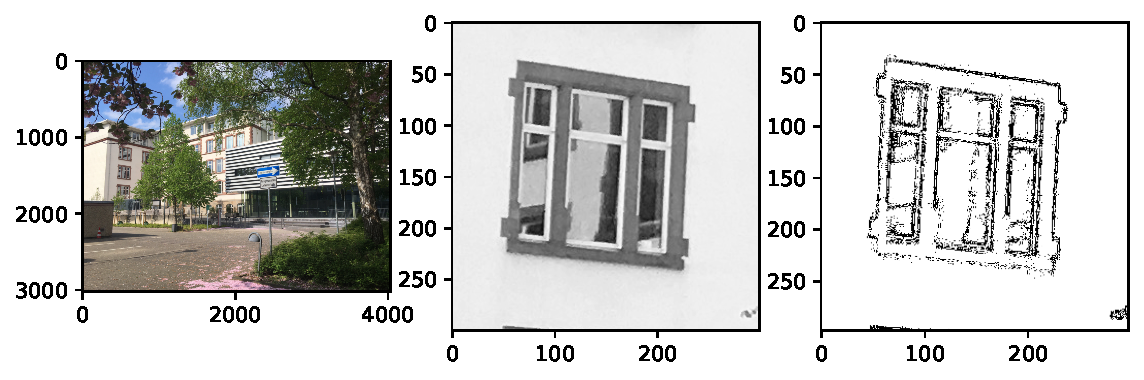
\includegraphics{books/w-python-numpy-grundlagen/skript/array_images_files/figure-pdf/cell-9-output-1.pdf}

Wir können damit ganz klar die Formen des Fensters erkennen.

Wollen wir zum Beispiel eine Farbkomponente bearbeiten und dann das Bild
wieder zusammensetzen, benötigen wir die Funktion
\texttt{np.dstack((rot,\ grün,\ blau)).astype(\textquotesingle{}uint8\textquotesingle{})},
wobei \texttt{rot}, \texttt{grün}und \texttt{blau} die jeweiligen
2D-Arrays sind. Versuchen wir nun die grüne Farbe aus dem Baum links zu
entfernen.

Wichtig ist, dass die Daten nach dem Zusammensetzen im Format
\texttt{uint8} vorliegen, deswegen die Methode
\texttt{.astype(\textquotesingle{}uint8\textquotesingle{})}.

\begin{Shaded}
\begin{Highlighting}[]
\NormalTok{data }\OperatorTok{=}\NormalTok{ plt.imread(}\StringTok{\textquotesingle{}01{-}daten/campus\_haspel.jpeg\textquotesingle{}}\NormalTok{)}

\CommentTok{\# Speichern der einzelnen Farben in Arrays}
\NormalTok{rot }\OperatorTok{=}\NormalTok{ np.array(data[:, :, }\DecValTok{0}\NormalTok{], dtype}\OperatorTok{=}\BuiltInTok{float}\NormalTok{)}
\NormalTok{gruen }\OperatorTok{=}\NormalTok{ np.array(data[:, :, }\DecValTok{1}\NormalTok{], dtype}\OperatorTok{=}\BuiltInTok{float}\NormalTok{)}
\NormalTok{blau }\OperatorTok{=}\NormalTok{ np.array(data[:, :, }\DecValTok{2}\NormalTok{], dtype}\OperatorTok{=}\BuiltInTok{float}\NormalTok{)}

\CommentTok{\# Setzen wir den Bereich des linken Baumes im Array auf 0}
\NormalTok{gruen\_neu }\OperatorTok{=}\NormalTok{ gruen.copy()}
\NormalTok{gruen\_neu[}\DecValTok{800}\NormalTok{:}\DecValTok{2000}\NormalTok{, }\DecValTok{700}\NormalTok{:}\DecValTok{1700}\NormalTok{] }\OperatorTok{=} \DecValTok{0}

\NormalTok{zusammengesetzt }\OperatorTok{=}\NormalTok{ np.dstack((rot, gruen\_neu, blau)).astype(}\StringTok{\textquotesingle{}uint8\textquotesingle{}}\NormalTok{)}

\NormalTok{plt.figure(figsize}\OperatorTok{=}\NormalTok{(}\DecValTok{8}\NormalTok{, }\DecValTok{5}\NormalTok{))}

\NormalTok{ax }\OperatorTok{=}\NormalTok{ plt.subplot(}\DecValTok{1}\NormalTok{, }\DecValTok{2}\NormalTok{, }\DecValTok{1}\NormalTok{)}
\NormalTok{ax.imshow(data, cmap}\OperatorTok{=}\StringTok{"Greys\_r"}\NormalTok{)}

\NormalTok{ax }\OperatorTok{=}\NormalTok{ plt.subplot(}\DecValTok{1}\NormalTok{, }\DecValTok{2}\NormalTok{, }\DecValTok{2}\NormalTok{)}
\NormalTok{ax.imshow(zusammengesetzt)}
\end{Highlighting}
\end{Shaded}

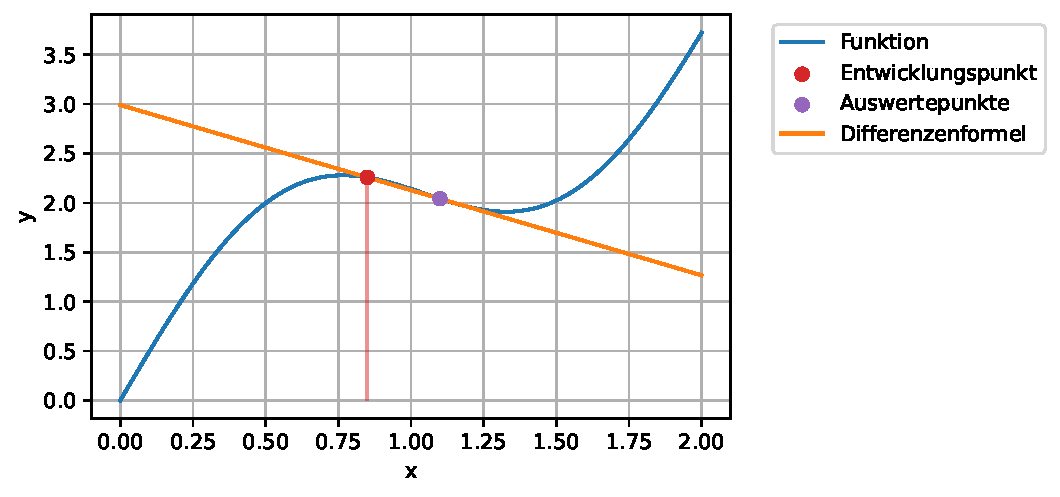
\includegraphics{books/w-python-numpy-grundlagen/skript/array_images_files/figure-pdf/cell-10-output-1.pdf}

\begin{tcolorbox}[enhanced jigsaw, breakable, opacityback=0, left=2mm, coltitle=black, leftrule=.75mm, colframe=quarto-callout-tip-color-frame, opacitybacktitle=0.6, toprule=.15mm, bottomtitle=1mm, titlerule=0mm, toptitle=1mm, title=\textcolor{quarto-callout-tip-color}{\faLightbulb}\hspace{0.5em}{Zwischenübung: Bilder bearbeiten}, colbacktitle=quarto-callout-tip-color!10!white, arc=.35mm, bottomrule=.15mm, rightrule=.15mm, colback=white]

Lesen Sie folgendes Bild vom Haspel Campus in Wuppertal ein:
\href{https://firedynamics.github.io/LectureComputerScience/_downloads/592f1fc843fc7c01bdcad17bf85ec15c/campus_haspel.jpeg}{Bild}

Extrahieren Sie den blauen Anteil und lassen Sie sich die Zeile in der
Mitte des Bildes ausgeben, so wie einen beliebigen Bildauschnitt.

\begin{tcolorbox}[enhanced jigsaw, breakable, opacityback=0, left=2mm, coltitle=black, leftrule=.75mm, colframe=quarto-callout-caution-color-frame, opacitybacktitle=0.6, toprule=.15mm, bottomtitle=1mm, titlerule=0mm, toptitle=1mm, title={Lösung}, colbacktitle=quarto-callout-caution-color!10!white, arc=.35mm, bottomrule=.15mm, rightrule=.15mm, colback=white]

\begin{Shaded}
\begin{Highlighting}[]
\ImportTok{import}\NormalTok{ numpy }\ImportTok{as}\NormalTok{ np}
\ImportTok{import}\NormalTok{ matplotlib.pyplot }\ImportTok{as}\NormalTok{ plt}

\NormalTok{data }\OperatorTok{=}\NormalTok{ plt.imread(}\StringTok{\textquotesingle{}01{-}daten/campus\_haspel.jpeg\textquotesingle{}}\NormalTok{)}

\NormalTok{form }\OperatorTok{=}\NormalTok{  data.shape}
\BuiltInTok{print}\NormalTok{( }\StringTok{"Form:"}\NormalTok{, data.shape )}

\NormalTok{blau }\OperatorTok{=}\NormalTok{  data[:,:,}\DecValTok{2}\NormalTok{]}
\NormalTok{plt.imshow(blau, cmap}\OperatorTok{=}\StringTok{\textquotesingle{}Blues\textquotesingle{}}\NormalTok{)}

\NormalTok{zeile }\OperatorTok{=}\NormalTok{  data[}\BuiltInTok{int}\NormalTok{(form[}\DecValTok{0}\NormalTok{]}\OperatorTok{/}\DecValTok{2}\NormalTok{),:,}\DecValTok{2}\NormalTok{]}
\BuiltInTok{print}\NormalTok{(zeile)}

\NormalTok{ausschnitt }\OperatorTok{=}\NormalTok{  data[}\DecValTok{10}\NormalTok{:}\DecValTok{50}\NormalTok{,}\DecValTok{10}\NormalTok{:}\DecValTok{50}\NormalTok{,:]}
\NormalTok{plt.imshow(ausschnitt)}
\end{Highlighting}
\end{Shaded}

\begin{verbatim}
Form: (3024, 4032, 3)
[221 220 220 ...  28  28  28]
\end{verbatim}

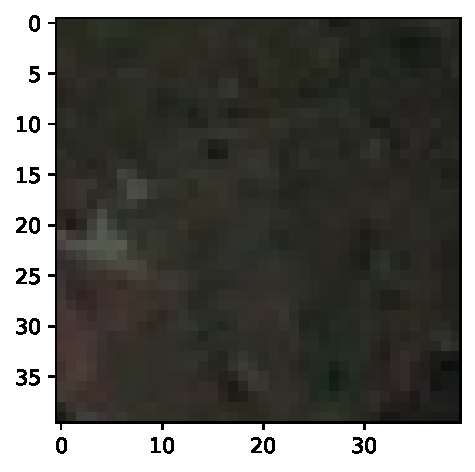
\includegraphics{books/w-python-numpy-grundlagen/skript/array_images_files/figure-pdf/cell-11-output-2.pdf}

\end{tcolorbox}

\end{tcolorbox}

\chapter{Lernzielkontrolle}\label{lernzielkontrolle}

Herzlich willkommen zur Lernzielkontrolle!

Diese Selbstlernkontrolle dient dazu, Ihr Verständnis der bisher
behandelten Themen zu überprüfen und Ihnen die Möglichkeit zu geben,
Ihren Lernfortschritt eigenständig zu bewerten. Sie ist so konzipiert,
dass Sie Ihre Stärken und Schwächen erkennen und gezielt an den
Bereichen arbeiten können, die noch verbessert werden müssen.

Es stehen hier zwei Möglichkeiten zur Verfügung ihr Wissen zu prüfen.
Sie können das Quiz benutzen, welches Sie automatisch durch die
verschiedenen Themen führt. ALternativ finden Sie darunter normale Frage
wie Sie bisher im Skript verwendet wurden.

Bitte nehmen Sie sich ausreichend Zeit für die Bearbeitung der Fragen
und gehen Sie diese in Ruhe durch. Seien Sie ehrlich zu sich selbst und
versuchen Sie, die Aufgaben ohne Hilfsmittel zu lösen, um ein
realistisches Bild Ihres aktuellen Wissensstands zu erhalten. Sollten
Sie bei einer Frage Schwierigkeiten haben, ist dies ein Hinweis darauf,
dass Sie in diesem Bereich noch weiter üben sollten.

Viel Erfolg bei der Bearbeitung und beim weiteren Lernen!

\section*{Aufgabe 1}\label{aufgabe-1}
\addcontentsline{toc}{section}{Aufgabe 1}

\markright{Aufgabe 1}

Wie wird das NumPy-Paket typischerweise eingebunden?

\section*{Aufgabe 2}\label{aufgabe-2}
\addcontentsline{toc}{section}{Aufgabe 2}

\markright{Aufgabe 2}

Erstellen Sie mit Hilfe von NumPy die folgenden Arrays:

\begin{enumerate}
\def\labelenumi{\arabic{enumi}.}
\tightlist
\item
  Erstellen sie aus der Liste {[}1, 2, 3{]} ein numPy Array
\item
  Ein eindimensionales Array, das die Zahlen von 0 bis 9 enthält.
\item
  Ein zweidimensionales Array der Form 3×33×3, das nur aus Einsen
  besteht.
\item
  Ein eindimensionales Array, das die Zahlen von 10 bis 50
  (einschließlich) in Schritten von 5 enthält.
\end{enumerate}

\section*{Aufgabe 3}\label{aufgabe-3}
\addcontentsline{toc}{section}{Aufgabe 3}

\markright{Aufgabe 3}

Was ist der Unterschied zwischenden den Funktionen \texttt{np.ndim},
\texttt{np.shape} und \texttt{np.size}

\section*{Aufgabe 4}\label{aufgabe-4}
\addcontentsline{toc}{section}{Aufgabe 4}

\markright{Aufgabe 4}

Welchen Datentyp besitzt folgendes Array? Mit welcher Funktion kann ich
den Datentypen eines Arrays auslesen?

\begin{Shaded}
\begin{Highlighting}[]
\NormalTok{vector }\OperatorTok{=}\NormalTok{ np.array([ }\FloatTok{4.8}\NormalTok{,  }\FloatTok{8.2}\NormalTok{, }\FloatTok{15.6}\NormalTok{, }\FloatTok{16.6}\NormalTok{, }\FloatTok{23.2}\NormalTok{, }\FloatTok{42.8}\NormalTok{ ])}
\end{Highlighting}
\end{Shaded}

\section*{Aufgabe 5}\label{aufgabe-5}
\addcontentsline{toc}{section}{Aufgabe 5}

\markright{Aufgabe 5}

Führen Sie mit den folgenden zwei Arrays diese mathematischen
Operationen durch:

a = {[}5, 1, 3, 6, 4{]} und b = {[}6, 5, 2, 6, 9{]}

\begin{enumerate}
\def\labelenumi{\arabic{enumi}.}
\tightlist
\item
  Addieren Sie beide Arrays
\item
  Berechnen Sie das elementweise Produkt von a und b
\item
  Addieren Sie zu jedem Eintrag von a 3 dazu
\end{enumerate}

\section*{Aufgabe 6}\label{aufgabe-6}
\addcontentsline{toc}{section}{Aufgabe 6}

\markright{Aufgabe 6}

a = {[}9, 2, 3, 1, 3{]}

\begin{enumerate}
\def\labelenumi{\arabic{enumi}.}
\tightlist
\item
  Bestimmen Sie Mittelwert und Standardabweichung für das Array a
\item
  Bestimmen Sie Minimum und Maximum der Liste
\end{enumerate}

\section*{Aufgabe 7}\label{aufgabe-7}
\addcontentsline{toc}{section}{Aufgabe 7}

\markright{Aufgabe 7}

\begin{Shaded}
\begin{Highlighting}[]
\NormalTok{matrix }\OperatorTok{=}\NormalTok{ np.array([}
\NormalTok{    [ }\DecValTok{1}\NormalTok{,  }\DecValTok{2}\NormalTok{,  }\DecValTok{3}\NormalTok{,  }\DecValTok{4}\NormalTok{,  }\DecValTok{5}\NormalTok{],}
\NormalTok{    [ }\DecValTok{6}\NormalTok{,  }\DecValTok{7}\NormalTok{,  }\DecValTok{8}\NormalTok{,  }\DecValTok{9}\NormalTok{, }\DecValTok{10}\NormalTok{],}
\NormalTok{    [}\DecValTok{11}\NormalTok{, }\DecValTok{12}\NormalTok{, }\DecValTok{13}\NormalTok{, }\DecValTok{14}\NormalTok{, }\DecValTok{15}\NormalTok{],}
\NormalTok{    [}\DecValTok{16}\NormalTok{, }\DecValTok{17}\NormalTok{, }\DecValTok{18}\NormalTok{, }\DecValTok{19}\NormalTok{, }\DecValTok{20}\NormalTok{],}
\NormalTok{    [}\DecValTok{21}\NormalTok{, }\DecValTok{22}\NormalTok{, }\DecValTok{23}\NormalTok{, }\DecValTok{24}\NormalTok{, }\DecValTok{25}\NormalTok{]}
\NormalTok{])}
\end{Highlighting}
\end{Shaded}

\begin{enumerate}
\def\labelenumi{\arabic{enumi}.}
\tightlist
\item
  Extrahieren Sie die erste Zeile.
\item
  Extrahieren Sie die letzte Spalte.
\item
  Extrahieren Sie die Untermatrix, die aus den Zeilen 2 bis 4 und den
  Spalten 1 bis 3 besteht.
\end{enumerate}

\section*{Aufgabe 8}\label{aufgabe-8}
\addcontentsline{toc}{section}{Aufgabe 8}

\markright{Aufgabe 8}

\begin{Shaded}
\begin{Highlighting}[]
\NormalTok{array }\OperatorTok{=}\NormalTok{ np.arange(}\DecValTok{1}\NormalTok{, }\DecValTok{21}\NormalTok{)}
\end{Highlighting}
\end{Shaded}

\begin{enumerate}
\def\labelenumi{\arabic{enumi}.}
\tightlist
\item
  Ändern Sie die Form des Arrays in eine zweidimensionale Matrix der
  Form 4×5.
\item
  Ändern Sie die Form des Arrays in eine zweidimensionale Matrix der
  Form 5×4.
\item
  Ändern Sie die Form des Arrays in eine dreidimensionale Matrix der
  Form 2×2×5.
\item
  Flachen Sie das dreidimensionale Array aus Aufgabe 3 wieder zu einem
  eindimensionalen Array ab.
\item
  Transponieren Sie die 4×54×5-Matrix aus Aufgabe 1.
\end{enumerate}

\section*{Aufgabe 9}\label{aufgabe-9}
\addcontentsline{toc}{section}{Aufgabe 9}

\markright{Aufgabe 9}

Mit welchen zwei Funktionen können Daten aus einer Datei gelesen und in
einer Datei gespeichert werden?

\section*{Aufgabe 10}\label{aufgabe-10}
\addcontentsline{toc}{section}{Aufgabe 10}

\markright{Aufgabe 10}

Sie möchten aus einem Bild die Bilddaten einer Farkomponente isolieren.
Was müssen Sie dafür tun?

\begin{tcolorbox}[enhanced jigsaw, breakable, opacityback=0, left=2mm, coltitle=black, leftrule=.75mm, colframe=quarto-callout-caution-color-frame, opacitybacktitle=0.6, toprule=.15mm, bottomtitle=1mm, titlerule=0mm, toptitle=1mm, title={Lösung}, colbacktitle=quarto-callout-caution-color!10!white, arc=.35mm, bottomrule=.15mm, rightrule=.15mm, colback=white]

\subsection*{Aufgabe 1}\label{aufgabe-1-1}
\addcontentsline{toc}{subsection}{Aufgabe 1}

\begin{Shaded}
\begin{Highlighting}[]
\ImportTok{import}\NormalTok{ numpy }\ImportTok{as}\NormalTok{ np}
\end{Highlighting}
\end{Shaded}

\subsection*{Aufgabe 2}\label{aufgabe-2-1}
\addcontentsline{toc}{subsection}{Aufgabe 2}

\begin{Shaded}
\begin{Highlighting}[]
\CommentTok{\# 1.}
\NormalTok{np.array([}\DecValTok{1}\NormalTok{, }\DecValTok{2}\NormalTok{, }\DecValTok{3}\NormalTok{])}

\CommentTok{\# 2. }
\BuiltInTok{print}\NormalTok{(np.arange(}\DecValTok{10}\NormalTok{))}

\CommentTok{\# 3. }
\BuiltInTok{print}\NormalTok{(np.ones((}\DecValTok{3}\NormalTok{, }\DecValTok{3}\NormalTok{)))}

\CommentTok{\# 4. }
\BuiltInTok{print}\NormalTok{(np.arange(}\DecValTok{10}\NormalTok{, }\DecValTok{51}\NormalTok{, }\DecValTok{5}\NormalTok{))}
\end{Highlighting}
\end{Shaded}

\begin{verbatim}
[0 1 2 3 4 5 6 7 8 9]
[[1. 1. 1.]
 [1. 1. 1.]
 [1. 1. 1.]]
[10 15 20 25 30 35 40 45 50]
\end{verbatim}

\subsection*{Aufgabe 3}\label{aufgabe-3-1}
\addcontentsline{toc}{subsection}{Aufgabe 3}

\texttt{np.ndim}: Gibt die Anzahl der Dimensionen zurück
\texttt{np.shape}: Gibt die Längen der einzelnen Dimensionen wieder
\texttt{np.size}: Gibt die Anzahl aller Elemente aus

\subsection*{Aufgabe 4}\label{aufgabe-4-1}
\addcontentsline{toc}{subsection}{Aufgabe 4}

Da es sich hier um Gleitkommazahlen handelt, ist der Datentyp
\texttt{float.64}.

\begin{Shaded}
\begin{Highlighting}[]
\NormalTok{vector }\OperatorTok{=}\NormalTok{ np.array([ }\FloatTok{4.8}\NormalTok{,  }\FloatTok{8.2}\NormalTok{, }\FloatTok{15.6}\NormalTok{, }\FloatTok{16.6}\NormalTok{, }\FloatTok{23.2}\NormalTok{, }\FloatTok{42.8}\NormalTok{ ])}
\BuiltInTok{print}\NormalTok{(vector.dtype)}
\end{Highlighting}
\end{Shaded}

\begin{verbatim}
float64
\end{verbatim}

\subsection*{Aufgabe 5}\label{aufgabe-5-1}
\addcontentsline{toc}{subsection}{Aufgabe 5}

\begin{Shaded}
\begin{Highlighting}[]
\NormalTok{a }\OperatorTok{=}\NormalTok{ np.array([}\DecValTok{5}\NormalTok{, }\DecValTok{1}\NormalTok{, }\DecValTok{3}\NormalTok{, }\DecValTok{6}\NormalTok{, }\DecValTok{4}\NormalTok{])}
\NormalTok{b }\OperatorTok{=}\NormalTok{ np.array([}\DecValTok{6}\NormalTok{, }\DecValTok{5}\NormalTok{, }\DecValTok{2}\NormalTok{, }\DecValTok{6}\NormalTok{, }\DecValTok{9}\NormalTok{])}

\CommentTok{\# 1.}
\NormalTok{ergebnis }\OperatorTok{=}\NormalTok{ a }\OperatorTok{+}\NormalTok{ b}
\BuiltInTok{print}\NormalTok{(}\StringTok{"Die Summe beider Vektoren ergibt: "}\NormalTok{, ergebnis) }

\CommentTok{\# 2.}
\NormalTok{ergebnis }\OperatorTok{=}\NormalTok{ a }\OperatorTok{*}\NormalTok{ b}
\BuiltInTok{print}\NormalTok{(}\StringTok{"Das Produkt beider Vektoren ergibt: "}\NormalTok{, ergebnis) }

\CommentTok{\# 3.}
\NormalTok{ergebnis }\OperatorTok{=}\NormalTok{ a }\OperatorTok{+} \DecValTok{3}
\BuiltInTok{print}\NormalTok{(}\StringTok{"Die Summe von a und 3 ergibt: "}\NormalTok{, ergebnis) }
\end{Highlighting}
\end{Shaded}

\begin{verbatim}
Die Summe beider Vektoren ergibt:  [11  6  5 12 13]
Das Produkt beider Vektoren ergibt:  [30  5  6 36 36]
Die Summe von a und 3 ergibt:  [8 4 6 9 7]
\end{verbatim}

\subsection*{Aufgabe 6}\label{aufgabe-6-1}
\addcontentsline{toc}{subsection}{Aufgabe 6}

\begin{Shaded}
\begin{Highlighting}[]
\NormalTok{a }\OperatorTok{=}\NormalTok{ np.array([}\DecValTok{9}\NormalTok{, }\DecValTok{2}\NormalTok{, }\DecValTok{3}\NormalTok{, }\DecValTok{1}\NormalTok{, }\DecValTok{3}\NormalTok{])}

\CommentTok{\# 1.}
\NormalTok{mittelwert }\OperatorTok{=}\NormalTok{ np.mean(a)}
\BuiltInTok{print}\NormalTok{(}\StringTok{"Der Mittelwert ist: "}\NormalTok{, mittelwert)}

\NormalTok{standardabweichung }\OperatorTok{=}\NormalTok{ np.std(a)}
\BuiltInTok{print}\NormalTok{(}\StringTok{"Die Standardabweichung von a beträgt: "}\NormalTok{, standardabweichung) }

\CommentTok{\# 2.}
\NormalTok{minimum }\OperatorTok{=}\NormalTok{ np.}\BuiltInTok{min}\NormalTok{(a)}
\BuiltInTok{print}\NormalTok{(}\StringTok{"Das Minimum beträgt: "}\NormalTok{, minimum)}

\NormalTok{maximum }\OperatorTok{=}\NormalTok{ np.}\BuiltInTok{max}\NormalTok{(a)}
\BuiltInTok{print}\NormalTok{(}\StringTok{"Das Maximum beträgt: "}\NormalTok{, maximum)}
\end{Highlighting}
\end{Shaded}

\begin{verbatim}
Der Mittelwert ist:  3.6
Die Standardabweichung von a beträgt:  2.8000000000000003
Das Minimum beträgt:  1
Das Maximum beträgt:  9
\end{verbatim}

\subsection*{Aufgabe 7}\label{aufgabe-7-1}
\addcontentsline{toc}{subsection}{Aufgabe 7}

\begin{Shaded}
\begin{Highlighting}[]
\NormalTok{matrix }\OperatorTok{=}\NormalTok{ np.array([}
\NormalTok{    [ }\DecValTok{1}\NormalTok{,  }\DecValTok{2}\NormalTok{,  }\DecValTok{3}\NormalTok{,  }\DecValTok{4}\NormalTok{,  }\DecValTok{5}\NormalTok{],}
\NormalTok{    [ }\DecValTok{6}\NormalTok{,  }\DecValTok{7}\NormalTok{,  }\DecValTok{8}\NormalTok{,  }\DecValTok{9}\NormalTok{, }\DecValTok{10}\NormalTok{],}
\NormalTok{    [}\DecValTok{11}\NormalTok{, }\DecValTok{12}\NormalTok{, }\DecValTok{13}\NormalTok{, }\DecValTok{14}\NormalTok{, }\DecValTok{15}\NormalTok{],}
\NormalTok{    [}\DecValTok{16}\NormalTok{, }\DecValTok{17}\NormalTok{, }\DecValTok{18}\NormalTok{, }\DecValTok{19}\NormalTok{, }\DecValTok{20}\NormalTok{],}
\NormalTok{    [}\DecValTok{21}\NormalTok{, }\DecValTok{22}\NormalTok{, }\DecValTok{23}\NormalTok{, }\DecValTok{24}\NormalTok{, }\DecValTok{25}\NormalTok{]}
\NormalTok{])}

\CommentTok{\# 1. Erste Zeile}
\BuiltInTok{print}\NormalTok{(matrix[}\DecValTok{0}\NormalTok{,:])}

\CommentTok{\# 2.}
\BuiltInTok{print}\NormalTok{(matrix[:,}\OperatorTok{{-}}\DecValTok{1}\NormalTok{])}

\CommentTok{\# 3.}
\BuiltInTok{print}\NormalTok{(matrix[}\DecValTok{1}\NormalTok{:}\DecValTok{4}\NormalTok{,}\DecValTok{0}\NormalTok{:}\DecValTok{3}\NormalTok{])}
\end{Highlighting}
\end{Shaded}

\begin{verbatim}
[1 2 3 4 5]
[ 5 10 15 20 25]
[[ 6  7  8]
 [11 12 13]
 [16 17 18]]
\end{verbatim}

\subsection*{Aufgabe 8}\label{aufgabe-8-1}
\addcontentsline{toc}{subsection}{Aufgabe 8}

\begin{Shaded}
\begin{Highlighting}[]
\NormalTok{array }\OperatorTok{=}\NormalTok{ np.arange(}\DecValTok{1}\NormalTok{, }\DecValTok{21}\NormalTok{)}

\CommentTok{\# 1. Ändern der Form in eine 4x5{-}Matrix}
\NormalTok{matrix\_4x5 }\OperatorTok{=}\NormalTok{ array.reshape(}\DecValTok{4}\NormalTok{, }\DecValTok{5}\NormalTok{)}

\CommentTok{\# 2. Ändern der Form in eine 5x4{-}Matrix}
\NormalTok{matrix\_5x4 }\OperatorTok{=}\NormalTok{ array.reshape(}\DecValTok{5}\NormalTok{, }\DecValTok{4}\NormalTok{)}

\CommentTok{\# 3. Ändern der Form in eine 2x2x5{-}Matrix}
\NormalTok{matrix\_2x2x5 }\OperatorTok{=}\NormalTok{ array.reshape(}\DecValTok{2}\NormalTok{, }\DecValTok{2}\NormalTok{, }\DecValTok{5}\NormalTok{)}

\CommentTok{\# 4. Abflachen der 2x2x5{-}Matrix zu einem eindimensionalen Array}
\NormalTok{flattened\_array }\OperatorTok{=}\NormalTok{ matrix\_2x2x5.flatten()}

\CommentTok{\# 5. Transponieren der 4x5{-}Matrix}
\NormalTok{transposed\_matrix }\OperatorTok{=}\NormalTok{ matrix\_4x5.T}

\CommentTok{\# Ausgabe der Ergebnisse (optional)}
\BuiltInTok{print}\NormalTok{(}\StringTok{"Originales Array:"}\NormalTok{, array)}
\BuiltInTok{print}\NormalTok{(}\StringTok{"4x5{-}Matrix:}\CharTok{\textbackslash{}n}\StringTok{"}\NormalTok{, matrix\_4x5)}
\BuiltInTok{print}\NormalTok{(}\StringTok{"5x4{-}Matrix:}\CharTok{\textbackslash{}n}\StringTok{"}\NormalTok{, matrix\_5x4)}
\BuiltInTok{print}\NormalTok{(}\StringTok{"2x2x5{-}Matrix:}\CharTok{\textbackslash{}n}\StringTok{"}\NormalTok{, matrix\_2x2x5)}
\BuiltInTok{print}\NormalTok{(}\StringTok{"Abgeflachtes Array:"}\NormalTok{, flattened\_array)}
\BuiltInTok{print}\NormalTok{(}\StringTok{"Transponierte 4x5{-}Matrix:}\CharTok{\textbackslash{}n}\StringTok{"}\NormalTok{, transposed\_matrix)}
\end{Highlighting}
\end{Shaded}

\begin{verbatim}
Originales Array: [ 1  2  3  4  5  6  7  8  9 10 11 12 13 14 15 16 17 18 19 20]
4x5-Matrix:
 [[ 1  2  3  4  5]
 [ 6  7  8  9 10]
 [11 12 13 14 15]
 [16 17 18 19 20]]
5x4-Matrix:
 [[ 1  2  3  4]
 [ 5  6  7  8]
 [ 9 10 11 12]
 [13 14 15 16]
 [17 18 19 20]]
2x2x5-Matrix:
 [[[ 1  2  3  4  5]
  [ 6  7  8  9 10]]

 [[11 12 13 14 15]
  [16 17 18 19 20]]]
Abgeflachtes Array: [ 1  2  3  4  5  6  7  8  9 10 11 12 13 14 15 16 17 18 19 20]
Transponierte 4x5-Matrix:
 [[ 1  6 11 16]
 [ 2  7 12 17]
 [ 3  8 13 18]
 [ 4  9 14 19]
 [ 5 10 15 20]]
\end{verbatim}

\subsection*{Aufgabe 9}\label{aufgabe-9-1}
\addcontentsline{toc}{subsection}{Aufgabe 9}

Die passenden Funktionen sind \texttt{np.loadtxt()} und
\texttt{np.savetxt()}.

\subsection*{Aufgabe 10}\label{aufgabe-10-1}
\addcontentsline{toc}{subsection}{Aufgabe 10}

Typischerweise sind Bilddaten große Matrizen wobei die Farben in drei
unterschieldichen Matrizen gespeichert werden. Dabei ist die
Farbreihenfolge oft ``Rot'', ``Grün'' und ``Blau''. Dementsprechen
müssen wir wenn wie Daten in der Matrix \texttt{data} gespeichert sind
mit Slicing eine Dimension auswählen: \texttt{data{[}:,:,0{]}}, wobei
die Zahl 0-2 für die jeweilige Farbe steht.

\end{tcolorbox}

\chapter{Übung}\label{uxfcbung}

\section{Aufgabe 1 Filmdatenbank}\label{aufgabe-1-filmdatenbank}

In der ersten Aufgabe wollen wir fiktive Daten für Filmbewertungen
untersuchen. Das Datenset ist dabei vereinfacht und beinhaltet folgende
Spalten:

\begin{enumerate}
\def\labelenumi{\arabic{enumi}.}
\tightlist
\item
  Film ID
\item
  Benutzer ID
\item
  Bewertung
\end{enumerate}

Hier ist das Datenset:

\begin{Shaded}
\begin{Highlighting}[]
\ImportTok{import}\NormalTok{ numpy }\ImportTok{as}\NormalTok{ np}

\NormalTok{bewertungen }\OperatorTok{=}\NormalTok{ np.array([}
\NormalTok{    [}\DecValTok{1}\NormalTok{, }\DecValTok{101}\NormalTok{, }\FloatTok{4.5}\NormalTok{],}
\NormalTok{    [}\DecValTok{1}\NormalTok{, }\DecValTok{102}\NormalTok{, }\FloatTok{3.0}\NormalTok{],}
\NormalTok{    [}\DecValTok{2}\NormalTok{, }\DecValTok{101}\NormalTok{, }\FloatTok{2.5}\NormalTok{],}
\NormalTok{    [}\DecValTok{2}\NormalTok{, }\DecValTok{103}\NormalTok{, }\FloatTok{4.0}\NormalTok{],}
\NormalTok{    [}\DecValTok{3}\NormalTok{, }\DecValTok{101}\NormalTok{, }\FloatTok{5.0}\NormalTok{],}
\NormalTok{    [}\DecValTok{3}\NormalTok{, }\DecValTok{104}\NormalTok{, }\FloatTok{3.5}\NormalTok{],}
\NormalTok{    [}\DecValTok{3}\NormalTok{, }\DecValTok{105}\NormalTok{, }\FloatTok{4.0}\NormalTok{]}
\NormalTok{])}
\end{Highlighting}
\end{Shaded}

\begin{tcolorbox}[enhanced jigsaw, breakable, opacityback=0, left=2mm, coltitle=black, leftrule=.75mm, colframe=quarto-callout-tip-color-frame, opacitybacktitle=0.6, toprule=.15mm, bottomtitle=1mm, titlerule=0mm, toptitle=1mm, title=\textcolor{quarto-callout-tip-color}{\faLightbulb}\hspace{0.5em}{a) Bestimmen Sie die jemals niedrigste und höchste Bewertung, die je
gegeben wurde}, colbacktitle=quarto-callout-tip-color!10!white, arc=.35mm, bottomrule=.15mm, rightrule=.15mm, colback=white]

\begin{tcolorbox}[enhanced jigsaw, breakable, opacityback=0, left=2mm, coltitle=black, leftrule=.75mm, colframe=quarto-callout-caution-color-frame, opacitybacktitle=0.6, toprule=.15mm, bottomtitle=1mm, titlerule=0mm, toptitle=1mm, title={Lösung}, colbacktitle=quarto-callout-caution-color!10!white, arc=.35mm, bottomrule=.15mm, rightrule=.15mm, colback=white]

\begin{Shaded}
\begin{Highlighting}[]
\NormalTok{niedrigste\_bewertung }\OperatorTok{=}\NormalTok{ np.}\BuiltInTok{min}\NormalTok{(bewertungen[:,}\DecValTok{2}\NormalTok{])}

\BuiltInTok{print}\NormalTok{(}\StringTok{"Die niedrigste jemals gegebene Bertung ist:"}\NormalTok{, niedrigste\_bewertung)}

\NormalTok{hoechste\_bewertung }\OperatorTok{=}\NormalTok{ np.}\BuiltInTok{max}\NormalTok{(bewertungen[:,}\DecValTok{2}\NormalTok{])}

\BuiltInTok{print}\NormalTok{(}\StringTok{"Die hoechste jemals gegebene Bertung ist:"}\NormalTok{, hoechste\_bewertung)}
\end{Highlighting}
\end{Shaded}

\begin{verbatim}
Die niedrigste jemals gegebene Bertung ist: 2.5
Die hoechste jemals gegebene Bertung ist: 5.0
\end{verbatim}

\end{tcolorbox}

\end{tcolorbox}

\begin{tcolorbox}[enhanced jigsaw, breakable, opacityback=0, left=2mm, coltitle=black, leftrule=.75mm, colframe=quarto-callout-tip-color-frame, opacitybacktitle=0.6, toprule=.15mm, bottomtitle=1mm, titlerule=0mm, toptitle=1mm, title=\textcolor{quarto-callout-tip-color}{\faLightbulb}\hspace{0.5em}{b) Nennen Sie alle Bewertungen für Film 1}, colbacktitle=quarto-callout-tip-color!10!white, arc=.35mm, bottomrule=.15mm, rightrule=.15mm, colback=white]

\begin{tcolorbox}[enhanced jigsaw, breakable, opacityback=0, left=2mm, coltitle=black, leftrule=.75mm, colframe=quarto-callout-caution-color-frame, opacitybacktitle=0.6, toprule=.15mm, bottomtitle=1mm, titlerule=0mm, toptitle=1mm, title={Lösung}, colbacktitle=quarto-callout-caution-color!10!white, arc=.35mm, bottomrule=.15mm, rightrule=.15mm, colback=white]

\begin{Shaded}
\begin{Highlighting}[]
\NormalTok{bewertungen\_film\_1 }\OperatorTok{=}\NormalTok{ bewertungen[np.where(bewertungen[:,}\DecValTok{0}\NormalTok{]}\OperatorTok{==}\DecValTok{1}\NormalTok{)]}

\BuiltInTok{print}\NormalTok{(}\StringTok{"Bewertungen für Film 1:}\CharTok{\textbackslash{}n}\StringTok{"}\NormalTok{, bewertungen\_film\_1)}
\end{Highlighting}
\end{Shaded}

\begin{verbatim}
Bewertungen für Film 1:
 [[  1.  101.    4.5]
 [  1.  102.    3. ]]
\end{verbatim}

\end{tcolorbox}

\end{tcolorbox}

\begin{tcolorbox}[enhanced jigsaw, breakable, opacityback=0, left=2mm, coltitle=black, leftrule=.75mm, colframe=quarto-callout-tip-color-frame, opacitybacktitle=0.6, toprule=.15mm, bottomtitle=1mm, titlerule=0mm, toptitle=1mm, title=\textcolor{quarto-callout-tip-color}{\faLightbulb}\hspace{0.5em}{c) Nennen Sie alle Bewertungen von Person 101}, colbacktitle=quarto-callout-tip-color!10!white, arc=.35mm, bottomrule=.15mm, rightrule=.15mm, colback=white]

\begin{tcolorbox}[enhanced jigsaw, breakable, opacityback=0, left=2mm, coltitle=black, leftrule=.75mm, colframe=quarto-callout-caution-color-frame, opacitybacktitle=0.6, toprule=.15mm, bottomtitle=1mm, titlerule=0mm, toptitle=1mm, title={Lösung}, colbacktitle=quarto-callout-caution-color!10!white, arc=.35mm, bottomrule=.15mm, rightrule=.15mm, colback=white]

\begin{Shaded}
\begin{Highlighting}[]
\NormalTok{bewertungen\_101 }\OperatorTok{=}\NormalTok{ bewertungen[np.where(bewertungen[:,}\DecValTok{1}\NormalTok{]}\OperatorTok{==}\DecValTok{101}\NormalTok{)]}

\BuiltInTok{print}\NormalTok{(}\StringTok{"Bewertungen von Person 101:}\CharTok{\textbackslash{}n}\StringTok{"}\NormalTok{, bewertungen\_101)}
\end{Highlighting}
\end{Shaded}

\begin{verbatim}
Bewertungen von Person 101:
 [[  1.  101.    4.5]
 [  2.  101.    2.5]
 [  3.  101.    5. ]]
\end{verbatim}

\end{tcolorbox}

\end{tcolorbox}

\begin{tcolorbox}[enhanced jigsaw, breakable, opacityback=0, left=2mm, coltitle=black, leftrule=.75mm, colframe=quarto-callout-tip-color-frame, opacitybacktitle=0.6, toprule=.15mm, bottomtitle=1mm, titlerule=0mm, toptitle=1mm, title=\textcolor{quarto-callout-tip-color}{\faLightbulb}\hspace{0.5em}{d) Berechnen Sie die mittlere Bewertung für jeden Film und geben Sie
diese nacheinander aus}, colbacktitle=quarto-callout-tip-color!10!white, arc=.35mm, bottomrule=.15mm, rightrule=.15mm, colback=white]

\begin{tcolorbox}[enhanced jigsaw, breakable, opacityback=0, left=2mm, coltitle=black, leftrule=.75mm, colframe=quarto-callout-caution-color-frame, opacitybacktitle=0.6, toprule=.15mm, bottomtitle=1mm, titlerule=0mm, toptitle=1mm, title={Lösung}, colbacktitle=quarto-callout-caution-color!10!white, arc=.35mm, bottomrule=.15mm, rightrule=.15mm, colback=white]

\begin{Shaded}
\begin{Highlighting}[]
\ControlFlowTok{for}\NormalTok{ ID }\KeywordTok{in}\NormalTok{ [}\DecValTok{1}\NormalTok{, }\DecValTok{2}\NormalTok{, }\DecValTok{3}\NormalTok{]:}

\NormalTok{    mittelwert }\OperatorTok{=}\NormalTok{ np.mean(bewertungen[np.where(bewertungen[:,}\DecValTok{0}\NormalTok{]}\OperatorTok{==}\NormalTok{ID),}\DecValTok{2}\NormalTok{])}

    \BuiltInTok{print}\NormalTok{(}\StringTok{"Die Mittlere Bewertung für Film"}\NormalTok{, ID, }\StringTok{"beträgt:"}\NormalTok{, mittelwert) }
\end{Highlighting}
\end{Shaded}

\begin{verbatim}
Die Mittlere Bewertung für Film 1 beträgt: 3.75
Die Mittlere Bewertung für Film 2 beträgt: 3.25
Die Mittlere Bewertung für Film 3 beträgt: 4.166666666666667
\end{verbatim}

\end{tcolorbox}

\end{tcolorbox}

\begin{tcolorbox}[enhanced jigsaw, breakable, opacityback=0, left=2mm, coltitle=black, leftrule=.75mm, colframe=quarto-callout-tip-color-frame, opacitybacktitle=0.6, toprule=.15mm, bottomtitle=1mm, titlerule=0mm, toptitle=1mm, title=\textcolor{quarto-callout-tip-color}{\faLightbulb}\hspace{0.5em}{e) Finden SIe den Film mit der höchsten Bewertung}, colbacktitle=quarto-callout-tip-color!10!white, arc=.35mm, bottomrule=.15mm, rightrule=.15mm, colback=white]

\begin{tcolorbox}[enhanced jigsaw, breakable, opacityback=0, left=2mm, coltitle=black, leftrule=.75mm, colframe=quarto-callout-caution-color-frame, opacitybacktitle=0.6, toprule=.15mm, bottomtitle=1mm, titlerule=0mm, toptitle=1mm, title={Lösung}, colbacktitle=quarto-callout-caution-color!10!white, arc=.35mm, bottomrule=.15mm, rightrule=.15mm, colback=white]

\begin{Shaded}
\begin{Highlighting}[]
\NormalTok{index\_hoechste\_bewertung }\OperatorTok{=}\NormalTok{ np.argmax(bewertungen[:,}\DecValTok{2}\NormalTok{])}

\BuiltInTok{print}\NormalTok{(bewertungen[index\_hoechste\_bewertung,:])}
\end{Highlighting}
\end{Shaded}

\begin{verbatim}
[  3. 101.   5.]
\end{verbatim}

\end{tcolorbox}

\end{tcolorbox}

\begin{tcolorbox}[enhanced jigsaw, breakable, opacityback=0, left=2mm, coltitle=black, leftrule=.75mm, colframe=quarto-callout-tip-color-frame, opacitybacktitle=0.6, toprule=.15mm, bottomtitle=1mm, titlerule=0mm, toptitle=1mm, title=\textcolor{quarto-callout-tip-color}{\faLightbulb}\hspace{0.5em}{f) Finden Sie die Person mit den meisten Bewertungen}, colbacktitle=quarto-callout-tip-color!10!white, arc=.35mm, bottomrule=.15mm, rightrule=.15mm, colback=white]

\begin{tcolorbox}[enhanced jigsaw, breakable, opacityback=0, left=2mm, coltitle=black, leftrule=.75mm, colframe=quarto-callout-caution-color-frame, opacitybacktitle=0.6, toprule=.15mm, bottomtitle=1mm, titlerule=0mm, toptitle=1mm, title={Lösung}, colbacktitle=quarto-callout-caution-color!10!white, arc=.35mm, bottomrule=.15mm, rightrule=.15mm, colback=white]

\begin{Shaded}
\begin{Highlighting}[]
\NormalTok{einzigartige\_person, anzahl }\OperatorTok{=}\NormalTok{ np.unique(bewertungen[:, }\DecValTok{1}\NormalTok{],return\_counts}\OperatorTok{=}\VariableTok{True}\NormalTok{)}

\NormalTok{meist\_aktiver\_person }\OperatorTok{=}\NormalTok{ einzigartige\_person[np.argmax(anzahl)]}

\BuiltInTok{print}\NormalTok{(}\StringTok{"Personen mit den meisten Bewertungen:"}\NormalTok{, meist\_aktiver\_person)}
\end{Highlighting}
\end{Shaded}

\begin{verbatim}
Personen mit den meisten Bewertungen: 101.0
\end{verbatim}

\end{tcolorbox}

\end{tcolorbox}

\begin{tcolorbox}[enhanced jigsaw, breakable, opacityback=0, left=2mm, coltitle=black, leftrule=.75mm, colframe=quarto-callout-tip-color-frame, opacitybacktitle=0.6, toprule=.15mm, bottomtitle=1mm, titlerule=0mm, toptitle=1mm, title=\textcolor{quarto-callout-tip-color}{\faLightbulb}\hspace{0.5em}{g) Nennen Sie alle Filme mit einer Wertung von 4 oder besser.}, colbacktitle=quarto-callout-tip-color!10!white, arc=.35mm, bottomrule=.15mm, rightrule=.15mm, colback=white]

\begin{tcolorbox}[enhanced jigsaw, breakable, opacityback=0, left=2mm, coltitle=black, leftrule=.75mm, colframe=quarto-callout-caution-color-frame, opacitybacktitle=0.6, toprule=.15mm, bottomtitle=1mm, titlerule=0mm, toptitle=1mm, title={Lösung}, colbacktitle=quarto-callout-caution-color!10!white, arc=.35mm, bottomrule=.15mm, rightrule=.15mm, colback=white]

\begin{Shaded}
\begin{Highlighting}[]
\NormalTok{index\_bewertung\_besser\_vier }\OperatorTok{=}\NormalTok{ bewertungen[:,}\DecValTok{2}\NormalTok{] }\OperatorTok{\textgreater{}=} \DecValTok{4}

\BuiltInTok{print}\NormalTok{(}\StringTok{"Filme mit einer Wertung von 4 oder besser:"}\NormalTok{)}

\BuiltInTok{print}\NormalTok{(bewertungen[index\_bewertung\_besser\_vier,:])}
\end{Highlighting}
\end{Shaded}

\begin{verbatim}
Filme mit einer Wertung von 4 oder besser:
[[  1.  101.    4.5]
 [  2.  103.    4. ]
 [  3.  101.    5. ]
 [  3.  105.    4. ]]
\end{verbatim}

\end{tcolorbox}

\end{tcolorbox}

\begin{tcolorbox}[enhanced jigsaw, breakable, opacityback=0, left=2mm, coltitle=black, leftrule=.75mm, colframe=quarto-callout-tip-color-frame, opacitybacktitle=0.6, toprule=.15mm, bottomtitle=1mm, titlerule=0mm, toptitle=1mm, title=\textcolor{quarto-callout-tip-color}{\faLightbulb}\hspace{0.5em}{h) Film Nr. 4 ist erschienen. Der Film wurde von Person 102 mit einer
Note von 3.5 bewertet. Fügen Sie diesen zur Datenbank hinzu.}, colbacktitle=quarto-callout-tip-color!10!white, arc=.35mm, bottomrule=.15mm, rightrule=.15mm, colback=white]

\begin{tcolorbox}[enhanced jigsaw, breakable, opacityback=0, left=2mm, coltitle=black, leftrule=.75mm, colframe=quarto-callout-caution-color-frame, opacitybacktitle=0.6, toprule=.15mm, bottomtitle=1mm, titlerule=0mm, toptitle=1mm, title={Lösung}, colbacktitle=quarto-callout-caution-color!10!white, arc=.35mm, bottomrule=.15mm, rightrule=.15mm, colback=white]

\begin{Shaded}
\begin{Highlighting}[]
\NormalTok{neue\_bewertung }\OperatorTok{=}\NormalTok{ np.array([}\DecValTok{4}\NormalTok{, }\DecValTok{102}\NormalTok{, }\FloatTok{3.5}\NormalTok{])}

\NormalTok{bewertungen }\OperatorTok{=}\NormalTok{ np.append(bewertungen, [neue\_bewertung], axis}\OperatorTok{=}\DecValTok{0}\NormalTok{)}

\BuiltInTok{print}\NormalTok{(bewertungen)}
\end{Highlighting}
\end{Shaded}

\begin{verbatim}
[[  1.  101.    4.5]
 [  1.  102.    3. ]
 [  2.  101.    2.5]
 [  2.  103.    4. ]
 [  3.  101.    5. ]
 [  3.  104.    3.5]
 [  3.  105.    4. ]
 [  4.  102.    3.5]]
\end{verbatim}

\end{tcolorbox}

\end{tcolorbox}

\begin{tcolorbox}[enhanced jigsaw, breakable, opacityback=0, left=2mm, coltitle=black, leftrule=.75mm, colframe=quarto-callout-tip-color-frame, opacitybacktitle=0.6, toprule=.15mm, bottomtitle=1mm, titlerule=0mm, toptitle=1mm, title=\textcolor{quarto-callout-tip-color}{\faLightbulb}\hspace{0.5em}{i) Person 102 hat sich Film Nr. 1 nochmal angesehen und hat das Ende
jetzt doch verstanden. Dementsprechend soll die Berwertung jetzt auf 5.0
geändert werden.}, colbacktitle=quarto-callout-tip-color!10!white, arc=.35mm, bottomrule=.15mm, rightrule=.15mm, colback=white]

\begin{tcolorbox}[enhanced jigsaw, breakable, opacityback=0, left=2mm, coltitle=black, leftrule=.75mm, colframe=quarto-callout-caution-color-frame, opacitybacktitle=0.6, toprule=.15mm, bottomtitle=1mm, titlerule=0mm, toptitle=1mm, title={Lösung}, colbacktitle=quarto-callout-caution-color!10!white, arc=.35mm, bottomrule=.15mm, rightrule=.15mm, colback=white]

\begin{Shaded}
\begin{Highlighting}[]
\NormalTok{bewertungen[(bewertungen[:, }\DecValTok{0}\NormalTok{] }\OperatorTok{==} \DecValTok{1}\NormalTok{) }\OperatorTok{\&} 
\NormalTok{            (bewertungen[:, }\DecValTok{1}\NormalTok{] }\OperatorTok{==} \DecValTok{102}\NormalTok{), }\DecValTok{2}\NormalTok{] }\OperatorTok{=} \FloatTok{5.0}

\BuiltInTok{print}\NormalTok{(}\StringTok{"Aktualisieren der Bewertung:}\CharTok{\textbackslash{}n}\StringTok{"}\NormalTok{, bewertungen)}
\end{Highlighting}
\end{Shaded}

\begin{verbatim}
Aktualisieren der Bewertung:
 [[  1.  101.    4.5]
 [  1.  102.    5. ]
 [  2.  101.    2.5]
 [  2.  103.    4. ]
 [  3.  101.    5. ]
 [  3.  104.    3.5]
 [  3.  105.    4. ]
 [  4.  102.    3.5]]
\end{verbatim}

\end{tcolorbox}

\end{tcolorbox}

\section{Aufgabe 2 - Kryptographie -
Caesar-Chiffre}\label{aufgabe-2---kryptographie---caesar-chiffre}

In dieser Aufgabe wollen wir Text sowohl ver- als auch entschlüsseln.

Jedes Zeichen hat über die sogenannte ASCII-Tabelle einen Zahlenwert
zugeordnet.

\begin{longtable}[]{@{}llll@{}}
\caption{Ascii-Tabelle}\label{tbl-ascii}\tabularnewline
\toprule\noalign{}
Buchstabe & ASCII Code & Buchstabe & ASCII Code \\
\midrule\noalign{}
\endfirsthead
\toprule\noalign{}
Buchstabe & ASCII Code & Buchstabe & ASCII Code \\
\midrule\noalign{}
\endhead
\bottomrule\noalign{}
\endlastfoot
a & 97 & n & 110 \\
b & 98 & o & 111 \\
c & 99 & p & 112 \\
d & 100 & q & 113 \\
e & 101 & r & 114 \\
f & 102 & s & 115 \\
g & 103 & t & 116 \\
h & 104 & u & 117 \\
i & 105 & v & 118 \\
j & 106 & w & 119 \\
k & 107 & x & 120 \\
l & 108 & y & 121 \\
m & 109 & z & 122 \\
\end{longtable}

Der Einfachheit halber ist im Folgenden schon der Code zur Umwandlung
von Buchstaben in Zahlenwerten und wieder zurück aufgeführt. Außerdem
beschränken wir uns auf Texte mit kleinen Buchstaben.

Ihre Aufgabe ist nun die Zahlenwerte zu verändern.

Zunächste wollen wir eine einfache Caesar-Chiffre anwenden. Dabei werden
alle Buchstaben um eine gewisse Anzahl verschoben. Ist Beispielsweise
der der Verschlüsselungswert ``1'' wird aus einem A ein B, einem M, ein
N. Ist der Wert ``4'' wird aus einem A ein E und aus einem M ein Q. Die
Verschiebung findet zyklisch statt, das heißt bei einer Verschiebung von
1 wird aus einem Z ein A.

\begin{Shaded}
\begin{Highlighting}[]
\ImportTok{import}\NormalTok{ numpy }\ImportTok{as}\NormalTok{ np}

\CommentTok{\# Funktion, die einen Buchstaben in ihren ASCII{-}Wert umwandelt}
\KeywordTok{def}\NormalTok{ buchstabe\_zu\_ascii(c):}
    \ControlFlowTok{return}\NormalTok{ np.array([}\BuiltInTok{ord}\NormalTok{(c)])}

\CommentTok{\# Funktion, die einen ASCII{-}Wert in den passenden Buchstaben umwandelt}
\KeywordTok{def}\NormalTok{ ascii\_zu\_buchstabe(a):}
    \ControlFlowTok{return} \BuiltInTok{chr}\NormalTok{(a)}
\end{Highlighting}
\end{Shaded}

\begin{tcolorbox}[enhanced jigsaw, breakable, opacityback=0, left=2mm, coltitle=black, leftrule=.75mm, colframe=quarto-callout-tip-color-frame, opacitybacktitle=0.6, toprule=.15mm, bottomtitle=1mm, titlerule=0mm, toptitle=1mm, title=\textcolor{quarto-callout-tip-color}{\faLightbulb}\hspace{0.5em}{1. Überlegen Sie sich zunächst wie man diese zyklische Verschiebung
mathematisch ausdrücken könnte (Hinweis: Modulo Rechnung)}, colbacktitle=quarto-callout-tip-color!10!white, arc=.35mm, bottomrule=.15mm, rightrule=.15mm, colback=white]

\begin{tcolorbox}[enhanced jigsaw, breakable, opacityback=0, left=2mm, coltitle=black, leftrule=.75mm, colframe=quarto-callout-caution-color-frame, opacitybacktitle=0.6, toprule=.15mm, bottomtitle=1mm, titlerule=0mm, toptitle=1mm, title={Lösung}, colbacktitle=quarto-callout-caution-color!10!white, arc=.35mm, bottomrule=.15mm, rightrule=.15mm, colback=white]

\[ \textrm{ASCII}_{\textrm{verschoben}} = (\textrm{ASCII} - 97 + \textrm{Versatz}) \textrm{ mod } 26 + 97\]

\end{tcolorbox}

\end{tcolorbox}

\begin{tcolorbox}[enhanced jigsaw, breakable, opacityback=0, left=2mm, coltitle=black, leftrule=.75mm, colframe=quarto-callout-tip-color-frame, opacitybacktitle=0.6, toprule=.15mm, bottomtitle=1mm, titlerule=0mm, toptitle=1mm, title=\textcolor{quarto-callout-tip-color}{\faLightbulb}\hspace{0.5em}{2. Schreiben Sie Code der mit einer Schleife alle Zeichen umwandelt.}, colbacktitle=quarto-callout-tip-color!10!white, arc=.35mm, bottomrule=.15mm, rightrule=.15mm, colback=white]

Zunächst sollen alle Zeichen in Ascii Code umgewandelt werden. Dann wird
die Formel auf die Zahlenwerte angewendet und schlussendlich in einer
dritten schleife wieder alle Werte in Buchstaben übersetzt.

\begin{tcolorbox}[enhanced jigsaw, breakable, opacityback=0, left=2mm, coltitle=black, leftrule=.75mm, colframe=quarto-callout-caution-color-frame, opacitybacktitle=0.6, toprule=.15mm, bottomtitle=1mm, titlerule=0mm, toptitle=1mm, title={Lösung}, colbacktitle=quarto-callout-caution-color!10!white, arc=.35mm, bottomrule=.15mm, rightrule=.15mm, colback=white]

\begin{Shaded}
\begin{Highlighting}[]
\ImportTok{import}\NormalTok{ numpy }\ImportTok{as}\NormalTok{ np}

\CommentTok{\# Funktion, die einen Buchstaben in ihren ASCII{-}Wert umwandelt}
\KeywordTok{def}\NormalTok{ buchstabe\_zu\_ascii(c):}
    \ControlFlowTok{return} \BuiltInTok{ord}\NormalTok{(c)}

\CommentTok{\# Funktion, die einen ASCII{-}Wert in den passenden Buchstaben umwandelt}
\KeywordTok{def}\NormalTok{ ascii\_zu\_buchstabe(a):}
    \ControlFlowTok{return} \BuiltInTok{chr}\NormalTok{(a)}

\NormalTok{klartext }\OperatorTok{=} \StringTok{"abrakadabra"}
\NormalTok{versatz }\OperatorTok{=} \DecValTok{3}

\NormalTok{umgewandelter\_text }\OperatorTok{=}\NormalTok{ []}
\NormalTok{verschluesselte\_zahl }\OperatorTok{=}\NormalTok{ []}
\NormalTok{verschluesselter\_text}\OperatorTok{=}\NormalTok{ []}



\ControlFlowTok{for}\NormalTok{ buchstabe }\KeywordTok{in}\NormalTok{ klartext:}
\NormalTok{    umgewandelter\_text.append(buchstabe\_zu\_ascii(buchstabe))}
\BuiltInTok{print}\NormalTok{(umgewandelter\_text)}


\ControlFlowTok{for}\NormalTok{ zahl }\KeywordTok{in}\NormalTok{ umgewandelter\_text:    }
\NormalTok{    verschluesselt }\OperatorTok{=}\NormalTok{ (zahl }\OperatorTok{{-}} \DecValTok{97} \OperatorTok{+}\NormalTok{ versatz) }\OperatorTok{\%} \DecValTok{26} \OperatorTok{+} \DecValTok{97}
\NormalTok{    verschluesselte\_zahl.append(verschluesselt)}
\BuiltInTok{print}\NormalTok{(verschluesselte\_zahl)}


\ControlFlowTok{for}\NormalTok{ zahl }\KeywordTok{in}\NormalTok{ verschluesselte\_zahl:    }
\NormalTok{    verschluesselter\_text.append(ascii\_zu\_buchstabe(zahl))}
\BuiltInTok{print}\NormalTok{(verschluesselter\_text)}
\end{Highlighting}
\end{Shaded}

\begin{verbatim}
[97, 98, 114, 97, 107, 97, 100, 97, 98, 114, 97]
[100, 101, 117, 100, 110, 100, 103, 100, 101, 117, 100]
['d', 'e', 'u', 'd', 'n', 'd', 'g', 'd', 'e', 'u', 'd']
\end{verbatim}

\end{tcolorbox}

\end{tcolorbox}

\begin{tcolorbox}[enhanced jigsaw, breakable, opacityback=0, left=2mm, coltitle=black, leftrule=.75mm, colframe=quarto-callout-tip-color-frame, opacitybacktitle=0.6, toprule=.15mm, bottomtitle=1mm, titlerule=0mm, toptitle=1mm, title=\textcolor{quarto-callout-tip-color}{\faLightbulb}\hspace{0.5em}{3. Ersetzen Sie die Schleife, indem Sie die Rechenoperation mit einem
NumPy-Array durchführen}, colbacktitle=quarto-callout-tip-color!10!white, arc=.35mm, bottomrule=.15mm, rightrule=.15mm, colback=white]

\begin{tcolorbox}[enhanced jigsaw, breakable, opacityback=0, left=2mm, coltitle=black, leftrule=.75mm, colframe=quarto-callout-caution-color-frame, opacitybacktitle=0.6, toprule=.15mm, bottomtitle=1mm, titlerule=0mm, toptitle=1mm, title={Lösung}, colbacktitle=quarto-callout-caution-color!10!white, arc=.35mm, bottomrule=.15mm, rightrule=.15mm, colback=white]

\begin{Shaded}
\begin{Highlighting}[]
\ImportTok{import}\NormalTok{ numpy }\ImportTok{as}\NormalTok{ np}

\CommentTok{\# Funktion, die einen Buchstaben in ihren ASCII{-}Wert umwandelt}
\KeywordTok{def}\NormalTok{ buchstabe\_zu\_ascii(c):}
    \ControlFlowTok{return} \BuiltInTok{ord}\NormalTok{(c)}

\CommentTok{\# Funktion, die einen ASCII{-}Wert in den passenden Buchstaben umwandelt}
\KeywordTok{def}\NormalTok{ ascii\_zu\_buchstabe(a):}
    \ControlFlowTok{return} \BuiltInTok{chr}\NormalTok{(a)}

\NormalTok{klartext }\OperatorTok{=} \StringTok{"abrakadabra"}
\NormalTok{versatz }\OperatorTok{=} \DecValTok{3}

\NormalTok{umgewandelter\_text }\OperatorTok{=}\NormalTok{ []}
\NormalTok{verschluesselte\_zahl }\OperatorTok{=}\NormalTok{ []}
\NormalTok{verschluesselter\_text}\OperatorTok{=}\NormalTok{ []}



\ControlFlowTok{for}\NormalTok{ buchstabe }\KeywordTok{in}\NormalTok{ klartext:}
\NormalTok{    umgewandelter\_text.append(buchstabe\_zu\_ascii(buchstabe))}
\BuiltInTok{print}\NormalTok{(umgewandelter\_text)}

\NormalTok{umgewandelter\_text }\OperatorTok{=}\NormalTok{ np.array(umgewandelter\_text)}
\NormalTok{verschluesselte\_zahl }\OperatorTok{=}\NormalTok{ (umgewandelter\_text }\OperatorTok{{-}} \DecValTok{97} \OperatorTok{+}\NormalTok{ versatz) }\OperatorTok{\%} \DecValTok{26} \OperatorTok{+} \DecValTok{97}
\BuiltInTok{print}\NormalTok{(verschluesselte\_zahl)}

\ControlFlowTok{for}\NormalTok{ zahl }\KeywordTok{in}\NormalTok{ verschluesselte\_zahl:    }
\NormalTok{    verschluesselter\_text.append(ascii\_zu\_buchstabe(zahl))}
\BuiltInTok{print}\NormalTok{(verschluesselter\_text)}
\end{Highlighting}
\end{Shaded}

\begin{verbatim}
[97, 98, 114, 97, 107, 97, 100, 97, 98, 114, 97]
[100 101 117 100 110 100 103 100 101 117 100]
['d', 'e', 'u', 'd', 'n', 'd', 'g', 'd', 'e', 'u', 'd']
\end{verbatim}

\end{tcolorbox}

\end{tcolorbox}

\begin{tcolorbox}[enhanced jigsaw, breakable, opacityback=0, left=2mm, coltitle=black, leftrule=.75mm, colframe=quarto-callout-tip-color-frame, opacitybacktitle=0.6, toprule=.15mm, bottomtitle=1mm, titlerule=0mm, toptitle=1mm, title=\textcolor{quarto-callout-tip-color}{\faLightbulb}\hspace{0.5em}{4. Schreiben sie den Code so um, dass der verschlüsselte Text
entschlüsselt wird.}, colbacktitle=quarto-callout-tip-color!10!white, arc=.35mm, bottomrule=.15mm, rightrule=.15mm, colback=white]

\begin{tcolorbox}[enhanced jigsaw, breakable, opacityback=0, left=2mm, coltitle=black, leftrule=.75mm, colframe=quarto-callout-caution-color-frame, opacitybacktitle=0.6, toprule=.15mm, bottomtitle=1mm, titlerule=0mm, toptitle=1mm, title={Lösung}, colbacktitle=quarto-callout-caution-color!10!white, arc=.35mm, bottomrule=.15mm, rightrule=.15mm, colback=white]

\begin{Shaded}
\begin{Highlighting}[]
\ImportTok{import}\NormalTok{ numpy }\ImportTok{as}\NormalTok{ np}

\CommentTok{\# Funktion, die einen Buchstaben in ihren ASCII{-}Wert umwandelt}
\KeywordTok{def}\NormalTok{ buchstabe\_zu\_ascii(c):}
    \ControlFlowTok{return} \BuiltInTok{ord}\NormalTok{(c)}

\CommentTok{\# Funktion, die einen ASCII{-}Wert in den passenden Buchstaben umwandelt}
\KeywordTok{def}\NormalTok{ ascii\_zu\_buchstabe(a):}
    \ControlFlowTok{return} \BuiltInTok{chr}\NormalTok{(a)}


\NormalTok{versatz }\OperatorTok{=} \DecValTok{3}

\NormalTok{umgewandelter\_text }\OperatorTok{=}\NormalTok{ []}
\NormalTok{verschluesselte\_zahl }\OperatorTok{=}\NormalTok{ []}
\NormalTok{entschluesselter\_text}\OperatorTok{=}\NormalTok{ []}



\ControlFlowTok{for}\NormalTok{ buchstabe }\KeywordTok{in}\NormalTok{ verschluesselter\_text:}
\NormalTok{    umgewandelter\_text.append(buchstabe\_zu\_ascii(buchstabe))}
\BuiltInTok{print}\NormalTok{(umgewandelter\_text)}

\NormalTok{umgewandelter\_text }\OperatorTok{=}\NormalTok{ np.array(umgewandelter\_text)}
\NormalTok{verschluesselte\_zahl }\OperatorTok{=}\NormalTok{ (umgewandelter\_text }\OperatorTok{{-}} \DecValTok{97} \OperatorTok{{-}}\NormalTok{ versatz) }\OperatorTok{\%} \DecValTok{26} \OperatorTok{+} \DecValTok{97}
\BuiltInTok{print}\NormalTok{(verschluesselte\_zahl)}

\ControlFlowTok{for}\NormalTok{ zahl }\KeywordTok{in}\NormalTok{ verschluesselte\_zahl:    }
\NormalTok{    entschluesselter\_text.append(ascii\_zu\_buchstabe(zahl))}
\BuiltInTok{print}\NormalTok{(entschluesselter\_text)}
\end{Highlighting}
\end{Shaded}

\begin{verbatim}
[100, 101, 117, 100, 110, 100, 103, 100, 101, 117, 100]
[ 97  98 114  97 107  97 100  97  98 114  97]
['a', 'b', 'r', 'a', 'k', 'a', 'd', 'a', 'b', 'r', 'a']
\end{verbatim}

\end{tcolorbox}

\end{tcolorbox}

\chapter{Klausurfragen}\label{klausurfragen}

\section*{Aufgabe 1}\label{aufgabe-1-2}
\addcontentsline{toc}{section}{Aufgabe 1}

\markright{Aufgabe 1}

Ein rechteckiger Träger aus Beton wird entlang seiner Länge mit einer
gleichmäßig verteilten Last belastet. Die Spannungsverteilung entlang
der Länge des Trägers soll analysiert werden. Der Träger hat eine Länge
von 10 Metern und eine Breite von 0.3 Metern. Die Höhe des Trägers
beträgt 0.5 Meter. Die gleichmäßig verteilte Last beträgt 5000 N/m.

\begin{enumerate}
\def\labelenumi{\arabic{enumi}.}
\item
  Erstellen Sie ein NumPy-Array \texttt{x} mit 100 gleichmäßig
  verteilten Punkten entlang der Länge des Trägers von 0 bis 10 Metern.
\item
  Berechnen Sie die Biegemomente \(M(x)\) entlang der Länge des Trägers
  unter Verwendung der Formel: \[
  \left[M(x) = \frac{w \cdot x \cdot (L - x)}{2}\right]
  \] wobei \(w\) die verteilte Last (in N/m), \(x\) die Position entlang
  des Trägers (in m) und \(L\) die Länge des Trägers (in m) ist.
\item
  Berechnen Sie die maximale Biegespannung σmaxσmax\hspace{0pt} an jedem
  Punkt entlang des Trägers unter Verwendung der Formel: \[
  \left[\sigma_{\text{max}}(x) = \frac{M(x) \cdot c}{I}\right]
  \] wobei cc der Abstand von der neutralen Faser zur äußersten Faser
  des Trägers ist (in m) und \(I\) das Flächenträgheitsmoment ist. Das
  Flächenträgheitsmoment eines rechteckigen Querschnitts ist: \[
  \left[
  I = \frac{b \cdot h^3}{12}
  \right]
  \] wobei \(b\) die Breite (in m) und \(h\) die Höhe des Trägers (in m)
  ist.
\item
  Bestimmen SIe die maximale Biegespannung
\item
  Plotten Sie die Spannungsverteilung \(\sigma_{max}​(x)\) entlang der
  Länge des Trägers.
\end{enumerate}

\part{w-python-matplotlib}

\chapter*{Preamble}\label{preamble-1}
\addcontentsline{toc}{chapter}{Preamble}

\markboth{Preamble}{Preamble}

\phantomsection\label{Lizenz}
\begin{figure}

\begin{minipage}{0.20\linewidth}
\includegraphics{index_files/mediabag/by.png}\end{minipage}%
%
\begin{minipage}{0.80\linewidth}
Bausteine Computergestützter Datenanalyse. ``Werkzeugbaustein Plotting
in Python'' von Lukas Arnold, Simone Arnold, Florian Bagemihl, Matthias
Baitsch, Marc Fehr, Maik Poetzsch und Sebastian Seipel ist lizensiert
unter \href{https://creativecommons.org/licenses/by/4.0/deed.de}{CC BY
4.0}. Das Werk ist abrufbar unter
\url{https://github.com/bausteine-der-datenanalyse/w-python-plotting}.
Ausgenommen von der Lizenz sind alle Logos und anders gekennzeichneten
Inhalte. 2024\end{minipage}%

\end{figure}%

Zitiervorschlag

Arnold, Lukas, Simone Arnold, Matthias Baitsch, Marc Fehr, Maik
Poetzsch, und Sebastian Seipel. 2024. „Bausteine Computergestützter
Datenanalyse. Werkzeugbaustein Plotting in Python``.
\url{https://github.com/bausteine-der-datenanalyse/w-python-plotting}.

BibTeX-Vorlage

\begin{verbatim}
@misc{BCD-Styleguide-2024,
 title={Bausteine Computergestützter Datenanalyse. Werkzeugbaustein Plotting in Python},
 author={Arnold, Lukas and Arnold, Simone and Baitsch, Matthias and Fehr, Marc and Poetzsch, Maik and Seipel, Sebastian},
 year={2024},
 url={https://github.com/bausteine-der-datenanalyse/w-python-plotting}} 
\end{verbatim}

\chapter*{Intro}\label{intro-1}
\addcontentsline{toc}{chapter}{Intro}

\markboth{Intro}{Intro}

\section*{Voraussetzungen}\label{voraussetzungen-2}
\addcontentsline{toc}{section}{Voraussetzungen}

\markright{Voraussetzungen}

\begin{itemize}
\tightlist
\item
  Grundlagen Python
\item
  Einbinden von zusätzlichen Paketen
\end{itemize}

\section*{Verwendete Pakete und
Datensätze}\label{verwendete-pakete-und-datensuxe4tze-1}
\addcontentsline{toc}{section}{Verwendete Pakete und Datensätze}

\markright{Verwendete Pakete und Datensätze}

\begin{itemize}
\tightlist
\item
  matplotlib
\end{itemize}

\section*{Bearbeitungszeit}\label{bearbeitungszeit-1}
\addcontentsline{toc}{section}{Bearbeitungszeit}

\markright{Bearbeitungszeit}

Geschätzte Bearbeitungszeit: 1h

\section*{Lernziele}\label{lernziele-2}
\addcontentsline{toc}{section}{Lernziele}

\markright{Lernziele}

\begin{itemize}
\tightlist
\item
  Einleitung: wie visualisiere ich Daten in Python
\item
  Anpassen von Plots
\item
  Do's \& Dont's für wissenschaftliche Plots
\end{itemize}

\chapter{Einführung in Matplotlib}\label{einfuxfchrung-in-matplotlib}

Matplotlib ist eine der bekanntesten Bibliotheken zur
Datenvisualisierung in Python. Sie ermöglicht das Erstellen statischer,
animierter und interaktiver Diagramme mit hoher Flexibilität.

\section{Warum Matplotlib?}\label{warum-matplotlib}

\begin{itemize}
\tightlist
\item
  \textbf{Breite Unterstützung:} Funktioniert mit NumPy, Pandas und
  SciPy.
\item
  \textbf{Hohe Anpassbarkeit:} Vollständige Kontrolle über Diagramme.
\item
  \textbf{Integration in Jupyter Notebooks:} Ideal für interaktive
  Datenanalyse.
\item
  \textbf{Kompatibilität:} Unterstützt verschiedene Ausgabeformate (PNG,
  SVG, PDF etc.).
\end{itemize}

\section{Alternativen zu Matplotlib}\label{alternativen-zu-matplotlib}

Während Matplotlib leistungsstark ist, gibt es Alternativen, die für
bestimmte Zwecke besser geeignet sein können: - \textbf{Seaborn:}
Basiert auf Matplotlib, erleichtert statistische Visualisierung. -
\textbf{Plotly:} Erzeugt interaktive Plots, gut für Dashboards. -
\textbf{Bokeh:} Ideal für Web-Anwendungen mit interaktiven
Visualisierungen.

\section{Erstes Beispiel: Einfache Linie
plotten}\label{erstes-beispiel-einfache-linie-plotten}

\begin{Shaded}
\begin{Highlighting}[]
\ImportTok{import}\NormalTok{ matplotlib.pyplot }\ImportTok{as}\NormalTok{ plt}
\ImportTok{import}\NormalTok{ numpy }\ImportTok{as}\NormalTok{ np}

\CommentTok{\# Beispiel{-}Daten}
\NormalTok{t }\OperatorTok{=}\NormalTok{ np.linspace(}\DecValTok{0}\NormalTok{, }\DecValTok{10}\NormalTok{, }\DecValTok{100}\NormalTok{)}
\NormalTok{y }\OperatorTok{=}\NormalTok{ np.sin(t)}

\CommentTok{\# Erstellen des Plots}
\NormalTok{plt.plot(t, y, label}\OperatorTok{=}\StringTok{\textquotesingle{}sin(t)\textquotesingle{}}\NormalTok{)}
\NormalTok{plt.xlabel(}\StringTok{\textquotesingle{}Zeit (s)\textquotesingle{}}\NormalTok{)}
\NormalTok{plt.ylabel(}\StringTok{\textquotesingle{}Amplitude\textquotesingle{}}\NormalTok{)}
\NormalTok{plt.title(}\StringTok{\textquotesingle{}Einfaches Linien{-}Diagramm\textquotesingle{}}\NormalTok{)}
\NormalTok{plt.legend()}
\NormalTok{plt.show()}
\end{Highlighting}
\end{Shaded}

Dieses einfache Beispiel zeigt, wie man mit Matplotlib eine
\textbf{Sinuskurve} visualisieren kann.

\section{Nächste Schritte}\label{nuxe4chste-schritte}

Im nächsten Kapitel werden wir uns mit den verschiedenen Diagrammtypen
beschäftigen, die Matplotlib bietet.

\chapter{Diagrammtypen in Matplotlib}\label{diagrammtypen-in-matplotlib}

Matplotlib bietet eine Vielzahl von Diagrammtypen, die für
unterschiedliche Zwecke geeignet sind. In diesem Kapitel werden die
wichtigsten Diagrammtypen vorgestellt und ihre Anwendungsfälle erklärt.

\section{\texorpdfstring{1. Liniendiagramme
(\texttt{plt.plot()})}{1. Liniendiagramme (plt.plot())}}\label{liniendiagramme-plt.plot}

Liniendiagramme eignen sich hervorragend zur Darstellung von Trends über
Zeit.

\begin{Shaded}
\begin{Highlighting}[]
\ImportTok{import}\NormalTok{ matplotlib.pyplot }\ImportTok{as}\NormalTok{ plt}
\ImportTok{import}\NormalTok{ numpy }\ImportTok{as}\NormalTok{ np}

\NormalTok{t }\OperatorTok{=}\NormalTok{ np.linspace(}\DecValTok{0}\NormalTok{, }\DecValTok{10}\NormalTok{, }\DecValTok{100}\NormalTok{)}
\NormalTok{y }\OperatorTok{=}\NormalTok{ np.sin(t)}

\NormalTok{plt.plot(t, y, label}\OperatorTok{=}\StringTok{\textquotesingle{}sin(t)\textquotesingle{}}\NormalTok{, color}\OperatorTok{=}\StringTok{\textquotesingle{}b\textquotesingle{}}\NormalTok{)}
\NormalTok{plt.xlabel(}\StringTok{\textquotesingle{}Zeit (s)\textquotesingle{}}\NormalTok{)}
\NormalTok{plt.ylabel(}\StringTok{\textquotesingle{}Amplitude\textquotesingle{}}\NormalTok{)}
\NormalTok{plt.title(}\StringTok{\textquotesingle{}Liniendiagramm\textquotesingle{}}\NormalTok{)}
\NormalTok{plt.legend()}
\NormalTok{plt.show()}
\end{Highlighting}
\end{Shaded}

\includegraphics{books/w-python-matplotlib/skript/basic_plot_types_files/figure-pdf/cell-2-output-1.png}

\section{\texorpdfstring{2. Streudiagramme
(\texttt{plt.scatter()})}{2. Streudiagramme (plt.scatter())}}\label{streudiagramme-plt.scatter}

Streudiagramme werden verwendet, um Zusammenhänge zwischen zwei
Variablen darzustellen.

\begin{Shaded}
\begin{Highlighting}[]
\NormalTok{x }\OperatorTok{=}\NormalTok{ np.random.rand(}\DecValTok{50}\NormalTok{)}
\NormalTok{y }\OperatorTok{=}\NormalTok{ np.random.rand(}\DecValTok{50}\NormalTok{)}

\NormalTok{plt.scatter(x, y, color}\OperatorTok{=}\StringTok{\textquotesingle{}r\textquotesingle{}}\NormalTok{, alpha}\OperatorTok{=}\FloatTok{0.5}\NormalTok{)}
\NormalTok{plt.xlabel(}\StringTok{\textquotesingle{}Variable X\textquotesingle{}}\NormalTok{)}
\NormalTok{plt.ylabel(}\StringTok{\textquotesingle{}Variable Y\textquotesingle{}}\NormalTok{)}
\NormalTok{plt.title(}\StringTok{\textquotesingle{}Streudiagramm\textquotesingle{}}\NormalTok{)}
\NormalTok{plt.show()}
\end{Highlighting}
\end{Shaded}

\includegraphics{books/w-python-matplotlib/skript/basic_plot_types_files/figure-pdf/cell-3-output-1.png}

\section{\texorpdfstring{3. Balkendiagramme
(\texttt{plt.bar()})}{3. Balkendiagramme (plt.bar())}}\label{balkendiagramme-plt.bar}

Balkendiagramme eignen sich zur Darstellung kategorialer Daten.

\begin{Shaded}
\begin{Highlighting}[]
\NormalTok{kategorien }\OperatorTok{=}\NormalTok{ [}\StringTok{\textquotesingle{}A\textquotesingle{}}\NormalTok{, }\StringTok{\textquotesingle{}B\textquotesingle{}}\NormalTok{, }\StringTok{\textquotesingle{}C\textquotesingle{}}\NormalTok{, }\StringTok{\textquotesingle{}D\textquotesingle{}}\NormalTok{]}
\NormalTok{werte }\OperatorTok{=}\NormalTok{ [}\DecValTok{3}\NormalTok{, }\DecValTok{7}\NormalTok{, }\DecValTok{1}\NormalTok{, }\DecValTok{5}\NormalTok{]}

\NormalTok{plt.bar(kategorien, werte, color}\OperatorTok{=}\StringTok{\textquotesingle{}g\textquotesingle{}}\NormalTok{)}
\NormalTok{plt.xlabel(}\StringTok{\textquotesingle{}Kategorien\textquotesingle{}}\NormalTok{)}
\NormalTok{plt.ylabel(}\StringTok{\textquotesingle{}Wert\textquotesingle{}}\NormalTok{)}
\NormalTok{plt.title(}\StringTok{\textquotesingle{}Balkendiagramm\textquotesingle{}}\NormalTok{)}
\NormalTok{plt.show()}
\end{Highlighting}
\end{Shaded}

\includegraphics{books/w-python-matplotlib/skript/basic_plot_types_files/figure-pdf/cell-4-output-1.png}

\section{\texorpdfstring{4. Histogramme
(\texttt{plt.hist()})}{4. Histogramme (plt.hist())}}\label{histogramme-plt.hist}

Histogramme zeigen die Verteilung numerischer Daten.

\begin{Shaded}
\begin{Highlighting}[]
\NormalTok{daten }\OperatorTok{=}\NormalTok{ np.random.randn(}\DecValTok{1000}\NormalTok{)}
\NormalTok{plt.hist(daten, bins}\OperatorTok{=}\DecValTok{30}\NormalTok{, color}\OperatorTok{=}\StringTok{\textquotesingle{}purple\textquotesingle{}}\NormalTok{, alpha}\OperatorTok{=}\FloatTok{0.7}\NormalTok{)}
\NormalTok{plt.xlabel(}\StringTok{\textquotesingle{}Wert\textquotesingle{}}\NormalTok{)}
\NormalTok{plt.ylabel(}\StringTok{\textquotesingle{}Häufigkeit\textquotesingle{}}\NormalTok{)}
\NormalTok{plt.title(}\StringTok{\textquotesingle{}Histogramm\textquotesingle{}}\NormalTok{)}
\NormalTok{plt.show()}
\end{Highlighting}
\end{Shaded}

\includegraphics{books/w-python-matplotlib/skript/basic_plot_types_files/figure-pdf/cell-5-output-1.png}

\section{\texorpdfstring{5. Boxplots
(\texttt{plt.boxplot()})}{5. Boxplots (plt.boxplot())}}\label{boxplots-plt.boxplot}

Boxplots helfen, Ausreißer und die Verteilung von Daten zu
visualisieren.

\begin{Shaded}
\begin{Highlighting}[]
\NormalTok{daten }\OperatorTok{=}\NormalTok{ [np.random.randn(}\DecValTok{100}\NormalTok{) }\ControlFlowTok{for}\NormalTok{ \_ }\KeywordTok{in} \BuiltInTok{range}\NormalTok{(}\DecValTok{4}\NormalTok{)]}
\NormalTok{plt.boxplot(daten, labels}\OperatorTok{=}\NormalTok{[}\StringTok{\textquotesingle{}A\textquotesingle{}}\NormalTok{, }\StringTok{\textquotesingle{}B\textquotesingle{}}\NormalTok{, }\StringTok{\textquotesingle{}C\textquotesingle{}}\NormalTok{, }\StringTok{\textquotesingle{}D\textquotesingle{}}\NormalTok{])}
\NormalTok{plt.ylabel(}\StringTok{\textquotesingle{}Wert\textquotesingle{}}\NormalTok{)}
\NormalTok{plt.title(}\StringTok{\textquotesingle{}Boxplot\textquotesingle{}}\NormalTok{)}
\NormalTok{plt.show()}
\end{Highlighting}
\end{Shaded}

\begin{verbatim}
/tmp/ipykernel_4865/2728911591.py:2: MatplotlibDeprecationWarning: The 'labels' parameter of boxplot() has been renamed 'tick_labels' since Matplotlib 3.9; support for the old name will be dropped in 3.11.
  plt.boxplot(daten, labels=['A', 'B', 'C', 'D'])
\end{verbatim}

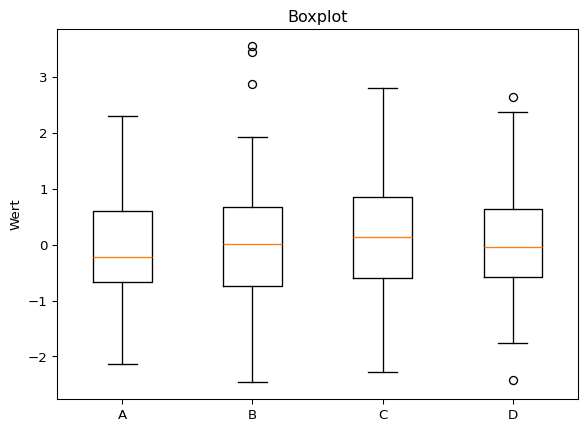
\includegraphics{books/w-python-matplotlib/skript/basic_plot_types_files/figure-pdf/cell-6-output-2.png}

\section{\texorpdfstring{6. Heatmaps
(\texttt{plt.imshow()})}{6. Heatmaps (plt.imshow())}}\label{heatmaps-plt.imshow}

Heatmaps eignen sich zur Darstellung von 2D-Daten.

\begin{Shaded}
\begin{Highlighting}[]
\NormalTok{daten }\OperatorTok{=}\NormalTok{ np.random.rand(}\DecValTok{10}\NormalTok{, }\DecValTok{10}\NormalTok{)}
\NormalTok{plt.imshow(daten, cmap}\OperatorTok{=}\StringTok{\textquotesingle{}coolwarm\textquotesingle{}}\NormalTok{, interpolation}\OperatorTok{=}\StringTok{\textquotesingle{}nearest\textquotesingle{}}\NormalTok{)}
\NormalTok{plt.colorbar()}
\NormalTok{plt.title(}\StringTok{\textquotesingle{}Heatmap\textquotesingle{}}\NormalTok{)}
\NormalTok{plt.show()}
\end{Highlighting}
\end{Shaded}

\includegraphics{books/w-python-matplotlib/skript/basic_plot_types_files/figure-pdf/cell-7-output-1.png}

\section{Fazit}\label{fazit}

Die Wahl des richtigen Diagrammtyps hängt von der Art der Daten und der
gewünschten Darstellung ab. Im nächsten Kapitel werden wir uns mit der
Anpassung und Gestaltung von Plots beschäftigen.

\chapter{Anpassung und Gestaltung von Plots in
Matplotlib}\label{anpassung-und-gestaltung-von-plots-in-matplotlib}

Ein gut gestaltetes Diagramm verbessert die Lesbarkeit und
Verständlichkeit der dargestellten Daten. In diesem Kapitel werden wir
verschiedene Möglichkeiten zur Anpassung und Gestaltung von Plots in
Matplotlib erkunden.

\section{1. Achsentitel und
Diagrammtitel}\label{achsentitel-und-diagrammtitel}

Klare Achsen- und Diagrammtitel sind essenziell für die Verständlichkeit
eines Plots.

\begin{Shaded}
\begin{Highlighting}[]
\ImportTok{import}\NormalTok{ matplotlib.pyplot }\ImportTok{as}\NormalTok{ plt}
\ImportTok{import}\NormalTok{ numpy }\ImportTok{as}\NormalTok{ np}

\NormalTok{t }\OperatorTok{=}\NormalTok{ np.linspace(}\DecValTok{0}\NormalTok{, }\DecValTok{10}\NormalTok{, }\DecValTok{100}\NormalTok{)}
\NormalTok{y }\OperatorTok{=}\NormalTok{ np.sin(t)}

\NormalTok{plt.plot(t, y, label}\OperatorTok{=}\StringTok{\textquotesingle{}sin(t)\textquotesingle{}}\NormalTok{, color}\OperatorTok{=}\StringTok{\textquotesingle{}b\textquotesingle{}}\NormalTok{)}
\NormalTok{plt.xlabel(}\StringTok{\textquotesingle{}Zeit (s)\textquotesingle{}}\NormalTok{, fontsize}\OperatorTok{=}\DecValTok{12}\NormalTok{)}
\NormalTok{plt.ylabel(}\StringTok{\textquotesingle{}Amplitude\textquotesingle{}}\NormalTok{, fontsize}\OperatorTok{=}\DecValTok{12}\NormalTok{)}
\NormalTok{plt.title(}\StringTok{\textquotesingle{}Liniendiagramm mit Beschriftung\textquotesingle{}}\NormalTok{, fontsize}\OperatorTok{=}\DecValTok{14}\NormalTok{)}
\NormalTok{plt.legend()}
\NormalTok{plt.show()}
\end{Highlighting}
\end{Shaded}

\includegraphics{books/w-python-matplotlib/skript/adapting_plots_files/figure-pdf/cell-2-output-1.png}

\section{2. Anpassung der Achsen}\label{anpassung-der-achsen}

Die Skalierung der Achsen sollte sinnvoll gewählt werden, um die Daten
bestmöglich darzustellen.

\begin{Shaded}
\begin{Highlighting}[]
\NormalTok{plt.plot(t, y, label}\OperatorTok{=}\StringTok{\textquotesingle{}sin(t)\textquotesingle{}}\NormalTok{, color}\OperatorTok{=}\StringTok{\textquotesingle{}b\textquotesingle{}}\NormalTok{)}
\NormalTok{plt.xlabel(}\StringTok{\textquotesingle{}Zeit (s)\textquotesingle{}}\NormalTok{)}
\NormalTok{plt.ylabel(}\StringTok{\textquotesingle{}Amplitude\textquotesingle{}}\NormalTok{)}
\NormalTok{plt.xlim(}\DecValTok{0}\NormalTok{, }\DecValTok{10}\NormalTok{)}
\NormalTok{plt.ylim(}\OperatorTok{{-}}\FloatTok{1.2}\NormalTok{, }\FloatTok{1.2}\NormalTok{)}
\NormalTok{plt.grid(}\VariableTok{True}\NormalTok{, linestyle}\OperatorTok{=}\StringTok{\textquotesingle{}{-}{-}\textquotesingle{}}\NormalTok{, alpha}\OperatorTok{=}\FloatTok{0.7}\NormalTok{)}
\NormalTok{plt.title(}\StringTok{\textquotesingle{}Liniendiagramm mit angepassten Achsen\textquotesingle{}}\NormalTok{)}
\NormalTok{plt.legend()}
\NormalTok{plt.show()}
\end{Highlighting}
\end{Shaded}

\includegraphics{books/w-python-matplotlib/skript/adapting_plots_files/figure-pdf/cell-3-output-1.png}

\section{3. Farben und Linienstile}\label{farben-und-linienstile}

Farben und Linienstile helfen dabei, wichtige Informationen im Plot
hervorzuheben.

\subsection{Wichtige Farben (Standardfarben in
Matplotlib)}\label{wichtige-farben-standardfarben-in-matplotlib}

\begin{longtable}[]{@{}lll@{}}
\toprule\noalign{}
Farbe & Kürzel & Beschreibung \\
\midrule\noalign{}
\endhead
\bottomrule\noalign{}
\endlastfoot
Blau & `b' & blue \\
Grün & `g' & green \\
Rot & `r' & red \\
Cyan & `c' & cyan \\
Magenta & `m' & magenta \\
Gelb & `y' & yellow \\
Schwarz & `k' & black \\
Weiß & `w' & white \\
\end{longtable}

\subsection{Wichtige Linienstile}\label{wichtige-linienstile}

\begin{longtable}[]{@{}lll@{}}
\toprule\noalign{}
Linienstil & Kürzel & Beschreibung \\
\midrule\noalign{}
\endhead
\bottomrule\noalign{}
\endlastfoot
Durchgezogen & `-' & Standardlinie \\
Gestrichelt & `--' & lange Striche \\
Gepunktet & `:' & nur Punkte \\
Strich-Punkt & `-.' & abwechselnd Strich-Punkt \\
\end{longtable}

\begin{Shaded}
\begin{Highlighting}[]
\NormalTok{plt.plot(t, np.sin(t), linestyle}\OperatorTok{=}\StringTok{\textquotesingle{}{-}\textquotesingle{}}\NormalTok{, color}\OperatorTok{=}\StringTok{\textquotesingle{}r\textquotesingle{}}\NormalTok{, label}\OperatorTok{=}\StringTok{\textquotesingle{}sin(t)\textquotesingle{}}\NormalTok{)}
\NormalTok{plt.plot(t, np.cos(t), linestyle}\OperatorTok{=}\StringTok{\textquotesingle{}{-}{-}\textquotesingle{}}\NormalTok{, color}\OperatorTok{=}\StringTok{\textquotesingle{}g\textquotesingle{}}\NormalTok{, label}\OperatorTok{=}\StringTok{\textquotesingle{}cos(t)\textquotesingle{}}\NormalTok{)}
\NormalTok{plt.xlabel(}\StringTok{\textquotesingle{}Zeit (s)\textquotesingle{}}\NormalTok{)}
\NormalTok{plt.ylabel(}\StringTok{\textquotesingle{}Amplitude\textquotesingle{}}\NormalTok{)}
\NormalTok{plt.title(}\StringTok{\textquotesingle{}Anpassung von Farben und Linienstilen\textquotesingle{}}\NormalTok{)}
\NormalTok{plt.legend()}
\NormalTok{plt.show()}
\end{Highlighting}
\end{Shaded}

\includegraphics{books/w-python-matplotlib/skript/adapting_plots_files/figure-pdf/cell-4-output-1.png}

\section{4. Mehrere Plots mit
Subplots}\label{mehrere-plots-mit-subplots}

Manchmal ist es sinnvoll, mehrere Diagramme in einer Abbildung
darzustellen.

\begin{Shaded}
\begin{Highlighting}[]
\NormalTok{fig, axs }\OperatorTok{=}\NormalTok{ plt.subplots(}\DecValTok{2}\NormalTok{, }\DecValTok{1}\NormalTok{, figsize}\OperatorTok{=}\NormalTok{(}\DecValTok{6}\NormalTok{, }\DecValTok{6}\NormalTok{))}
\NormalTok{axs[}\DecValTok{0}\NormalTok{].plot(t, np.sin(t), color}\OperatorTok{=}\StringTok{\textquotesingle{}b\textquotesingle{}}\NormalTok{)}
\NormalTok{axs[}\DecValTok{0}\NormalTok{].set\_title(}\StringTok{\textquotesingle{}Sinusfunktion\textquotesingle{}}\NormalTok{)}
\NormalTok{axs[}\DecValTok{1}\NormalTok{].plot(t, np.cos(t), color}\OperatorTok{=}\StringTok{\textquotesingle{}r\textquotesingle{}}\NormalTok{)}
\NormalTok{axs[}\DecValTok{1}\NormalTok{].set\_title(}\StringTok{\textquotesingle{}Kosinusfunktion\textquotesingle{}}\NormalTok{)}
\NormalTok{plt.tight\_layout()}
\NormalTok{plt.show()}
\end{Highlighting}
\end{Shaded}

\includegraphics{books/w-python-matplotlib/skript/adapting_plots_files/figure-pdf/cell-5-output-1.png}

\section{5. Speichern von Plots}\label{speichern-von-plots}

Man kann Diagramme in verschiedenen Formaten speichern.

\begin{Shaded}
\begin{Highlighting}[]
\NormalTok{plt.plot(t, y, label}\OperatorTok{=}\StringTok{\textquotesingle{}sin(t)\textquotesingle{}}\NormalTok{, color}\OperatorTok{=}\StringTok{\textquotesingle{}b\textquotesingle{}}\NormalTok{)}
\NormalTok{plt.xlabel(}\StringTok{\textquotesingle{}Zeit (s)\textquotesingle{}}\NormalTok{)}
\NormalTok{plt.ylabel(}\StringTok{\textquotesingle{}Amplitude\textquotesingle{}}\NormalTok{)}
\NormalTok{plt.title(}\StringTok{\textquotesingle{}Speicherung eines Plots\textquotesingle{}}\NormalTok{)}
\NormalTok{plt.legend()}
\NormalTok{plt.savefig(}\StringTok{\textquotesingle{}mein\_plot.png\textquotesingle{}}\NormalTok{, dpi}\OperatorTok{=}\DecValTok{300}\NormalTok{)}
\NormalTok{plt.show()}
\end{Highlighting}
\end{Shaded}

\includegraphics{books/w-python-matplotlib/skript/adapting_plots_files/figure-pdf/cell-6-output-1.png}

\section{Fazit}\label{fazit-1}

Durch geschickte Anpassungen lassen sich wissenschaftliche Plots
deutlich verbessern. Im nächsten Kapitel werden wir uns mit erweiterten
Techniken wie logarithmischen Skalen und Annotationen beschäftigen.

\chapter{Erweiterte Techniken in
Matplotlib}\label{erweiterte-techniken-in-matplotlib}

In diesem Kapitel betrachten wir einige fortgeschrittene Funktionen von
Matplotlib, die für die wissenschaftliche Datenvisualisierung besonders
nützlich sind.

\section{1. Logarithmische Skalen}\label{logarithmische-skalen}

Logarithmische Skalen werden oft verwendet, wenn Werte große
Größenordnungen umfassen.

\begin{Shaded}
\begin{Highlighting}[]
\ImportTok{import}\NormalTok{ matplotlib.pyplot }\ImportTok{as}\NormalTok{ plt}
\ImportTok{import}\NormalTok{ numpy }\ImportTok{as}\NormalTok{ np}

\NormalTok{x }\OperatorTok{=}\NormalTok{ np.logspace(}\FloatTok{0.1}\NormalTok{, }\DecValTok{2}\NormalTok{, }\DecValTok{100}\NormalTok{)}
\NormalTok{y }\OperatorTok{=}\NormalTok{ np.log10(x)}

\NormalTok{plt.plot(x, y, label}\OperatorTok{=}\StringTok{\textquotesingle{}log10(x)\textquotesingle{}}\NormalTok{, color}\OperatorTok{=}\StringTok{\textquotesingle{}b\textquotesingle{}}\NormalTok{)}
\NormalTok{plt.xscale(}\StringTok{\textquotesingle{}log\textquotesingle{}}\NormalTok{)}
\NormalTok{plt.xlabel(}\StringTok{\textquotesingle{}X{-}Wert (log{-}Skala)\textquotesingle{}}\NormalTok{)}
\NormalTok{plt.ylabel(}\StringTok{\textquotesingle{}Y{-}Wert\textquotesingle{}}\NormalTok{)}
\NormalTok{plt.title(}\StringTok{\textquotesingle{}Logarithmische Skalierung\textquotesingle{}}\NormalTok{)}
\NormalTok{plt.legend()}
\NormalTok{plt.grid(}\VariableTok{True}\NormalTok{, which}\OperatorTok{=}\StringTok{\textquotesingle{}both\textquotesingle{}}\NormalTok{, linestyle}\OperatorTok{=}\StringTok{\textquotesingle{}{-}{-}\textquotesingle{}}\NormalTok{, alpha}\OperatorTok{=}\FloatTok{0.7}\NormalTok{)}
\NormalTok{plt.show()}
\end{Highlighting}
\end{Shaded}

\includegraphics{books/w-python-matplotlib/skript/advanced_techniques_files/figure-pdf/cell-2-output-1.png}

\section{2. Twin-Achsen für verschiedene
Skalierungen}\label{twin-achsen-fuxfcr-verschiedene-skalierungen}

Manchmal möchte man zwei verschiedene y-Achsen in einem Plot darstellen.

\begin{Shaded}
\begin{Highlighting}[]
\NormalTok{x }\OperatorTok{=}\NormalTok{ np.linspace(}\DecValTok{0}\NormalTok{, }\DecValTok{10}\NormalTok{, }\DecValTok{100}\NormalTok{)}
\NormalTok{y1 }\OperatorTok{=}\NormalTok{ np.sin(x)}
\NormalTok{y2 }\OperatorTok{=}\NormalTok{ np.exp(x }\OperatorTok{/} \DecValTok{3}\NormalTok{)}

\NormalTok{fig, ax1 }\OperatorTok{=}\NormalTok{ plt.subplots()}
\NormalTok{ax2 }\OperatorTok{=}\NormalTok{ ax1.twinx()}
\NormalTok{ax1.plot(x, y1, }\StringTok{\textquotesingle{}g{-}\textquotesingle{}}\NormalTok{, label}\OperatorTok{=}\StringTok{\textquotesingle{}sin(x)\textquotesingle{}}\NormalTok{)}
\NormalTok{ax2.plot(x, y2, }\StringTok{\textquotesingle{}b{-}{-}\textquotesingle{}}\NormalTok{, label}\OperatorTok{=}\StringTok{\textquotesingle{}exp(x/3)\textquotesingle{}}\NormalTok{)}

\NormalTok{ax1.set\_xlabel(}\StringTok{\textquotesingle{}X{-}Wert\textquotesingle{}}\NormalTok{)}
\NormalTok{ax1.set\_ylabel(}\StringTok{\textquotesingle{}Sinus\textquotesingle{}}\NormalTok{, color}\OperatorTok{=}\StringTok{\textquotesingle{}g\textquotesingle{}}\NormalTok{)}
\NormalTok{ax2.set\_ylabel(}\StringTok{\textquotesingle{}Exponentiell\textquotesingle{}}\NormalTok{, color}\OperatorTok{=}\StringTok{\textquotesingle{}b\textquotesingle{}}\NormalTok{)}
\NormalTok{ax1.set\_title(}\StringTok{\textquotesingle{}Twin{-}Achsen für unterschiedliche Skalierungen\textquotesingle{}}\NormalTok{)}
\NormalTok{plt.show()}
\end{Highlighting}
\end{Shaded}

\includegraphics{books/w-python-matplotlib/skript/advanced_techniques_files/figure-pdf/cell-3-output-1.png}

\section{3. Annotationen in
Diagrammen}\label{annotationen-in-diagrammen}

Wichtige Punkte oder Werte in einem Diagramm können mit Annotationen
hervorgehoben werden.

\begin{Shaded}
\begin{Highlighting}[]
\NormalTok{x }\OperatorTok{=}\NormalTok{ np.linspace(}\DecValTok{0}\NormalTok{, }\DecValTok{10}\NormalTok{, }\DecValTok{100}\NormalTok{)}
\NormalTok{y }\OperatorTok{=}\NormalTok{ np.sin(x)}

\NormalTok{plt.plot(x, y, label}\OperatorTok{=}\StringTok{\textquotesingle{}sin(x)\textquotesingle{}}\NormalTok{)}
\NormalTok{plt.xlabel(}\StringTok{\textquotesingle{}X{-}Wert\textquotesingle{}}\NormalTok{)}
\NormalTok{plt.ylabel(}\StringTok{\textquotesingle{}Amplitude\textquotesingle{}}\NormalTok{)}
\NormalTok{plt.title(}\StringTok{\textquotesingle{}Annotationen in Matplotlib\textquotesingle{}}\NormalTok{)}
\NormalTok{plt.annotate(}\StringTok{\textquotesingle{}Maximalwert\textquotesingle{}}\NormalTok{, xy}\OperatorTok{=}\NormalTok{(np.pi}\OperatorTok{/}\DecValTok{2}\NormalTok{, }\DecValTok{1}\NormalTok{), xytext}\OperatorTok{=}\NormalTok{(}\DecValTok{2}\NormalTok{, }\FloatTok{1.2}\NormalTok{),}
\NormalTok{             arrowprops}\OperatorTok{=}\BuiltInTok{dict}\NormalTok{(facecolor}\OperatorTok{=}\StringTok{\textquotesingle{}red\textquotesingle{}}\NormalTok{, shrink}\OperatorTok{=}\FloatTok{0.05}\NormalTok{))}
\NormalTok{plt.legend()}
\NormalTok{plt.show()}
\end{Highlighting}
\end{Shaded}

\includegraphics{books/w-python-matplotlib/skript/advanced_techniques_files/figure-pdf/cell-4-output-1.png}

\section{Fazit}\label{fazit-2}

Diese erweiterten Funktionen helfen dabei, wissenschaftliche Plots noch
informativer zu gestalten. Im nächsten Kapitel werden wir Best Practices
und typische Fehler in der wissenschaftlichen Visualisierung betrachten.

\chapter{Best Practices in Matplotlib: Fehler und
Verbesserungen}\label{best-practices-in-matplotlib-fehler-und-verbesserungen}

In diesem Kapitel zeigen wir für häufige Problemstellungen jeweils ein
schlechtes und ein verbessertes Beispiel.

\section{1. Fehlende Beschriftungen}\label{fehlende-beschriftungen}

\subsection{❌ Schlechtes Beispiel}\label{schlechtes-beispiel}

\begin{Shaded}
\begin{Highlighting}[]
\ImportTok{import}\NormalTok{ matplotlib.pyplot }\ImportTok{as}\NormalTok{ plt}
\ImportTok{import}\NormalTok{ numpy }\ImportTok{as}\NormalTok{ np}

\NormalTok{x }\OperatorTok{=}\NormalTok{ np.linspace(}\DecValTok{0}\NormalTok{, }\DecValTok{10}\NormalTok{, }\DecValTok{100}\NormalTok{)}
\NormalTok{y }\OperatorTok{=}\NormalTok{ np.sin(x)}

\NormalTok{plt.plot(x, y)}
\NormalTok{plt.show()}
\end{Highlighting}
\end{Shaded}

\includegraphics{books/w-python-matplotlib/skript/scientific_plotting_files/figure-pdf/cell-2-output-1.png}

\subsection{✅ Besseres Beispiel}\label{besseres-beispiel}

\begin{Shaded}
\begin{Highlighting}[]
\NormalTok{plt.plot(x, y, label}\OperatorTok{=}\StringTok{\textquotesingle{}sin(x)\textquotesingle{}}\NormalTok{, color}\OperatorTok{=}\StringTok{\textquotesingle{}b\textquotesingle{}}\NormalTok{)}
\NormalTok{plt.xlabel(}\StringTok{\textquotesingle{}Zeit (s)\textquotesingle{}}\NormalTok{)}
\NormalTok{plt.ylabel(}\StringTok{\textquotesingle{}Amplitude\textquotesingle{}}\NormalTok{)}
\NormalTok{plt.title(}\StringTok{\textquotesingle{}Sinuskurve\textquotesingle{}}\NormalTok{)}
\NormalTok{plt.legend()}
\NormalTok{plt.show()}
\end{Highlighting}
\end{Shaded}

\includegraphics{books/w-python-matplotlib/skript/scientific_plotting_files/figure-pdf/cell-3-output-1.png}

\section{2. Ungünstige Farbwahl}\label{unguxfcnstige-farbwahl}

\subsection{❌ Schlechtes Beispiel}\label{schlechtes-beispiel-1}

\begin{Shaded}
\begin{Highlighting}[]
\NormalTok{plt.plot(x, y, color}\OperatorTok{=}\StringTok{\textquotesingle{}yellow\textquotesingle{}}\NormalTok{)}
\NormalTok{plt.show()}
\end{Highlighting}
\end{Shaded}

\includegraphics{books/w-python-matplotlib/skript/scientific_plotting_files/figure-pdf/cell-4-output-1.png}

\subsection{✅ Besseres Beispiel}\label{besseres-beispiel-1}

\begin{Shaded}
\begin{Highlighting}[]
\NormalTok{plt.plot(x, y, color}\OperatorTok{=}\StringTok{\textquotesingle{}darkblue\textquotesingle{}}\NormalTok{)}
\NormalTok{plt.grid(}\VariableTok{True}\NormalTok{, linestyle}\OperatorTok{=}\StringTok{\textquotesingle{}{-}{-}\textquotesingle{}}\NormalTok{, alpha}\OperatorTok{=}\FloatTok{0.7}\NormalTok{)}
\NormalTok{plt.title(}\StringTok{\textquotesingle{}Gute Kontraste für bessere Lesbarkeit\textquotesingle{}}\NormalTok{)}
\NormalTok{plt.show()}
\end{Highlighting}
\end{Shaded}

\includegraphics{books/w-python-matplotlib/skript/scientific_plotting_files/figure-pdf/cell-5-output-1.png}

\section{3. Keine sinnvolle
Achsenskalierung}\label{keine-sinnvolle-achsenskalierung}

\subsection{❌ Schlechtes Beispiel}\label{schlechtes-beispiel-2}

\begin{Shaded}
\begin{Highlighting}[]
\NormalTok{plt.plot(x, y)}
\NormalTok{plt.ylim(}\FloatTok{0.5}\NormalTok{, }\DecValTok{1}\NormalTok{)}
\NormalTok{plt.show()}
\end{Highlighting}
\end{Shaded}

\includegraphics{books/w-python-matplotlib/skript/scientific_plotting_files/figure-pdf/cell-6-output-1.png}

\subsection{✅ Besseres Beispiel}\label{besseres-beispiel-2}

\begin{Shaded}
\begin{Highlighting}[]
\NormalTok{plt.plot(x, y)}
\NormalTok{plt.ylim(}\OperatorTok{{-}}\FloatTok{1.2}\NormalTok{, }\FloatTok{1.2}\NormalTok{)}
\NormalTok{plt.xlim(}\DecValTok{0}\NormalTok{, }\DecValTok{10}\NormalTok{)}
\NormalTok{plt.grid(}\VariableTok{True}\NormalTok{)}
\NormalTok{plt.title(}\StringTok{\textquotesingle{}Sinnvolle Achsenskalierung\textquotesingle{}}\NormalTok{)}
\NormalTok{plt.show()}
\end{Highlighting}
\end{Shaded}

\includegraphics{books/w-python-matplotlib/skript/scientific_plotting_files/figure-pdf/cell-7-output-1.png}

\section{4. Überladung durch zu viele
Linien}\label{uxfcberladung-durch-zu-viele-linien}

\subsection{❌ Schlechtes Beispiel}\label{schlechtes-beispiel-3}

\begin{Shaded}
\begin{Highlighting}[]
\ControlFlowTok{for}\NormalTok{ i }\KeywordTok{in} \BuiltInTok{range}\NormalTok{(}\DecValTok{10}\NormalTok{):}
\NormalTok{    plt.plot(x, np.sin(x }\OperatorTok{+}\NormalTok{ i }\OperatorTok{*} \FloatTok{0.2}\NormalTok{))}
\NormalTok{plt.show()}
\end{Highlighting}
\end{Shaded}

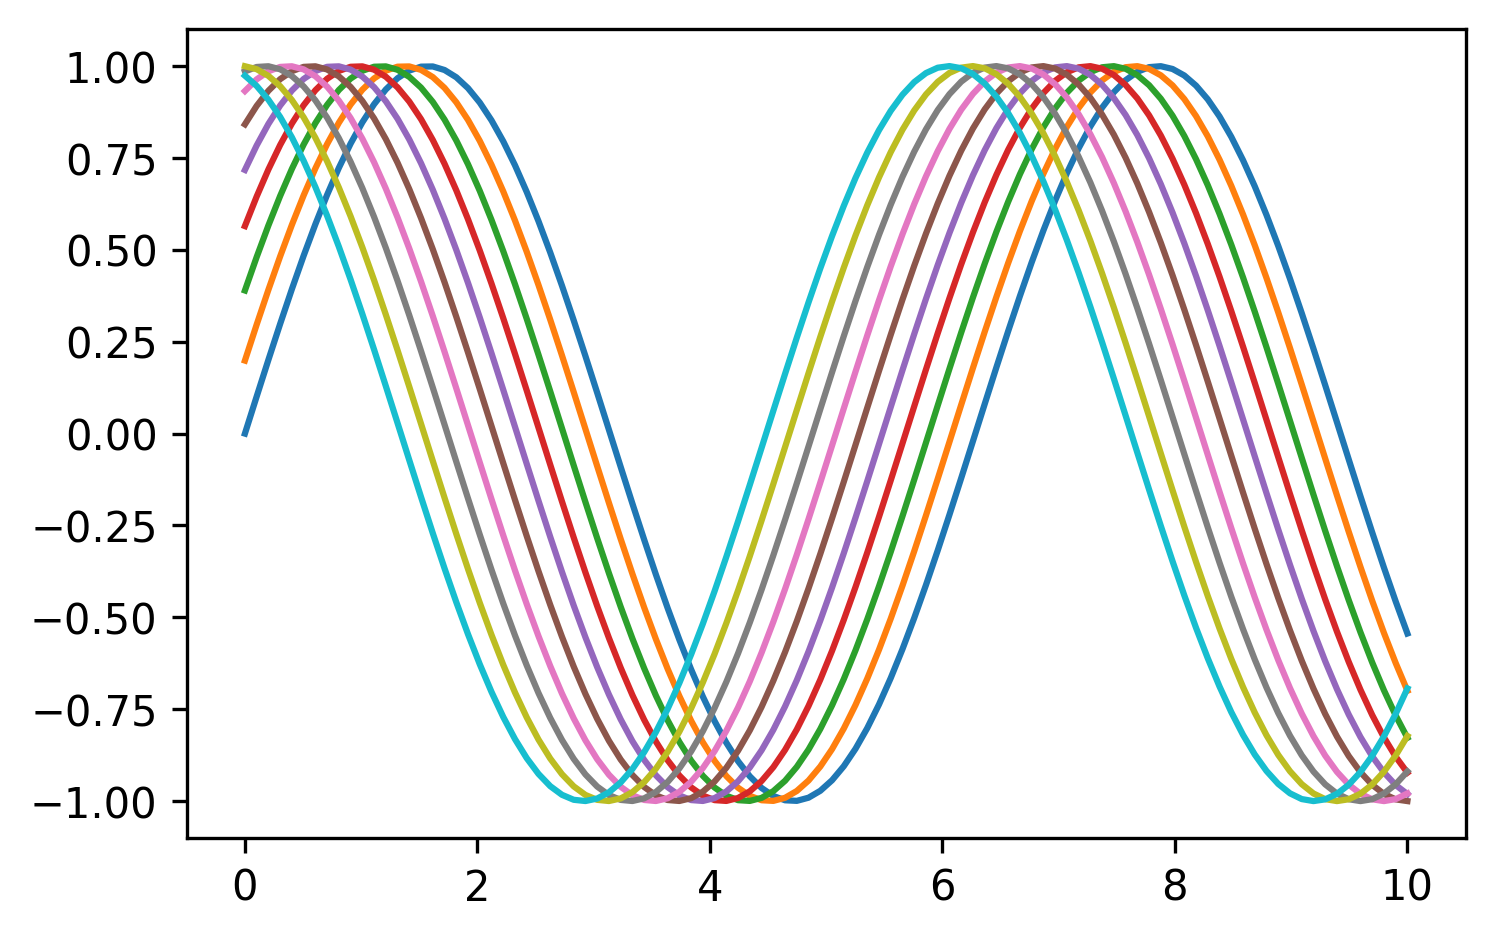
\includegraphics{books/w-python-matplotlib/skript/scientific_plotting_files/figure-pdf/cell-8-output-1.png}

\subsection{✅ Besseres Beispiel}\label{besseres-beispiel-3}

\begin{Shaded}
\begin{Highlighting}[]
\NormalTok{plt.plot(x, np.sin(x), label}\OperatorTok{=}\StringTok{\textquotesingle{}sin(x)\textquotesingle{}}\NormalTok{)}
\NormalTok{plt.plot(x, np.cos(x), label}\OperatorTok{=}\StringTok{\textquotesingle{}cos(x)\textquotesingle{}}\NormalTok{)}
\NormalTok{plt.legend()}
\NormalTok{plt.title(}\StringTok{\textquotesingle{}Weniger ist mehr: Reduzierte Informationsdichte\textquotesingle{}}\NormalTok{)}
\NormalTok{plt.grid(}\VariableTok{True}\NormalTok{)}
\NormalTok{plt.show()}
\end{Highlighting}
\end{Shaded}

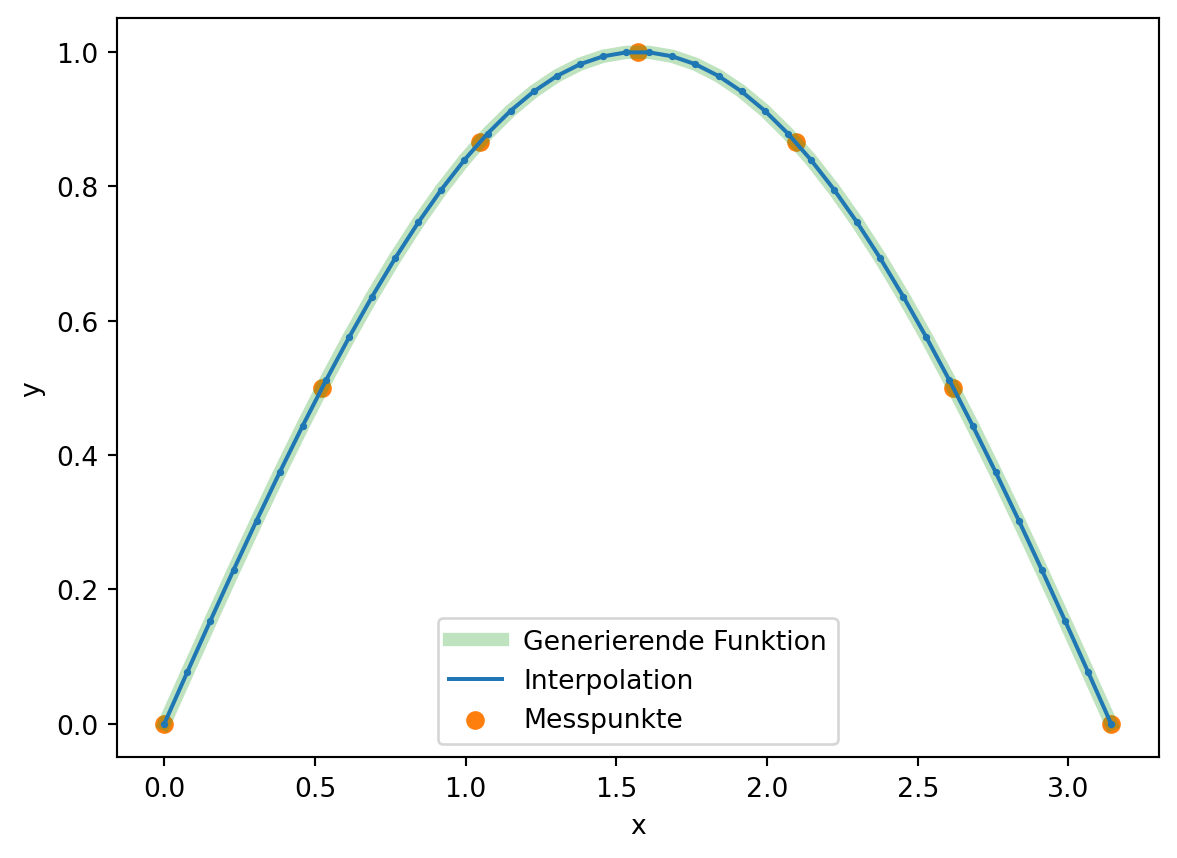
\includegraphics{books/w-python-matplotlib/skript/scientific_plotting_files/figure-pdf/cell-9-output-1.png}

\section{Fazit}\label{fazit-3}

Gute Plots zeichnen sich durch klare Beschriftungen, gute Lesbarkeit und
eine sinnvolle Informationsdichte aus.

\end{tcolorbox}




\end{document}
